\documentclass[pdftex,12pt,a4paper]{report}

\usepackage[portuguese,english]{babel}
\usepackage[T1]{fontenc} 
\usepackage[normalem]{ulem}
\useunder{\uline}{\ul}{}
\usepackage[table,xcdraw]{xcolor}
\usepackage[utf8]{inputenc}
\usepackage[pdftex]{graphicx}
\usepackage{minitoc}
\usepackage{hyperref}
\usepackage{indentfirst}
\usepackage[compact]{titlesec}
\usepackage{fancyhdr}
\usepackage{caption}
\usepackage{pgfplots}
\usepackage{pgfplotstable}
\usepackage{fixltx2e}
\usepackage{mathtools}
\usepackage{fancyhdr}
\usepackage{color}
\usepackage{sverb}
\usepackage[section]{placeins}
\usepackage{listings,xcolor}
\usepackage{inconsolata}
\definecolor{dkgreen}{rgb}{0,.6,0}
\definecolor{dkblue}{rgb}{0,0,.6}
\definecolor{dkyellow}{cmyk}{0,0,.8,.3}

\lstset{
  language        = php,
  basicstyle      = \small\ttfamily,
  keywordstyle    = \color{dkblue},
  stringstyle     = \color{red},
  identifierstyle = \color{dkgreen},
  commentstyle    = \color{gray},
  emph            =[1]{php},
  emphstyle       =[1]\color{black},
  emph            =[2]{if,and,or,else},
  emphstyle       =[2]\color{dkyellow}}
 
%Highlight
\newcommand{\shellcmd}[1]{\indent\indent\texttt{\footnotesize\# #1}\\}

\pagestyle{fancy}
\renewcommand*\thesection{\thechapter\arabic{section}}
\newcommand{\HRule}{\rule{\linewidth}{0.5mm}}
\begin{document}

\begin{titlepage}

\begin{center}


\includegraphics[width=0.15\textwidth]{./logo}\\[0.5cm]    

\textsc{\large Universidade de Aveiro \\[1cm]\large departamento de electrónica, telecomunicações e informática}\\[1cm]

\textsc{\large Gestão Integrada de Redes e Sistemas\\[1cm]}

\HRule \\[0.5cm]
{ \huge \bfseries RAID, NAS and SAN}\\[0.4cm]
{ \large \bfseries Exercício Prático}\\[0.4cm]
\HRule \\[1cm]

\textsc{\small{8240 - MESTRADO INTEGRADO EM ENGENHARIA DE COMPUTADORES E TELEMÁTICA}}\\[1cm]

\begin{minipage}{0.4\textwidth}

\begin{flushleft} \large
\href{mailto:rafael.ferreira@ua.pt}{António Rafael da \\ Costa Ferreira }
 \small{\\NMec: 67405}
\end{flushleft}
\end{minipage}
\begin{minipage}{0.4\textwidth}

\begin{flushright} \large
\href{mailto:rodrigocunha@ua.pt}{Rodrigo Lopes \\ da Cunha}
\small{\\NMec: 67800}
\end{flushright}
\end{minipage}\\[1cm]

{\large Docentes: Diogo Gomes,}\\
{\large \hspace{2.5cm} João Paulo Barraca}\\[0.5cm]


\vfill

{\large Março de 2016 \\ 2015-2016}

\end{center}

\end{titlepage} %Titulo do Relatorio
\renewcommand{\headrulewidth}{0pt}

%Cabeçalhos de rodapé
\fancyhead{}
\fancyfoot{}
\lhead{Docker Data Center}
\rhead{GIRS - 2015/2016}
\lfoot{Rafael Ferreira nmec: 67405 \\ Rodrigo Cunha nmec: 67800}
\rfoot{\thepage}

%Renomear Comandos
\renewcommand*\contentsname{Conteúdos}
\renewcommand*\figurename{Figura}
\renewcommand*\tablename{Tabela}

%Conteúdos, dar paragrafo
\tableofcontents
%Headers
\renewcommand{\headrulewidth}{0.15pt}
\renewcommand{\thechapter}{}

\clearpage

\section{Introdução}
% o que, porquê e o objetivo

O relatório reflete todos os passos no desenvolvimento das diferentes componentes, virtualização, armazenamento e monitorização, presentes no Docker Data Center, que está a ser desenvolvido no âmbito da disciplina de Gestão Integrada de Redes e Sistemas. 

\newpage

\section{Virtualização}

Após a apresentação sobre as várias soluções de virtualização foi dada a possibilidade de se escolher qual solução que se iria explorar durante o semestre.

Foi escolhido o Docker por ser uma tecnologia bastante recente e com um comunidade bastante ativa.

O objetivo será usando o Docker, simular uma infraestrutura virtual para um data center.

\subsection{Docker}

No Docker, os containers correm numa única máquina e partilham o mesmo kernel do sistema operativo de forma a que iniciem imediatamente e torne o uso da RAM mais eficiente.

As imagens são construídas com base em camadas de sistema de ficheiros para que seja possível partilhar ficheiros comuns, tornando o uso do disco e o download de imagens mais eficiente.

Os containers são baseados em "open standards" permitindo que os containers corram em praticamente todas as distribuições Linux e sistemas operativos Microsoft com suporte para todas as infraestruturas. Estes isolam as aplicações uns dos outros e a infraestrutura subjacente, proporcionando uma camada adicional de proteção para a aplicação.

\subsubsection{Comparação com Máquinas Virtuais}

\begin{figure}[!htb]
\center
 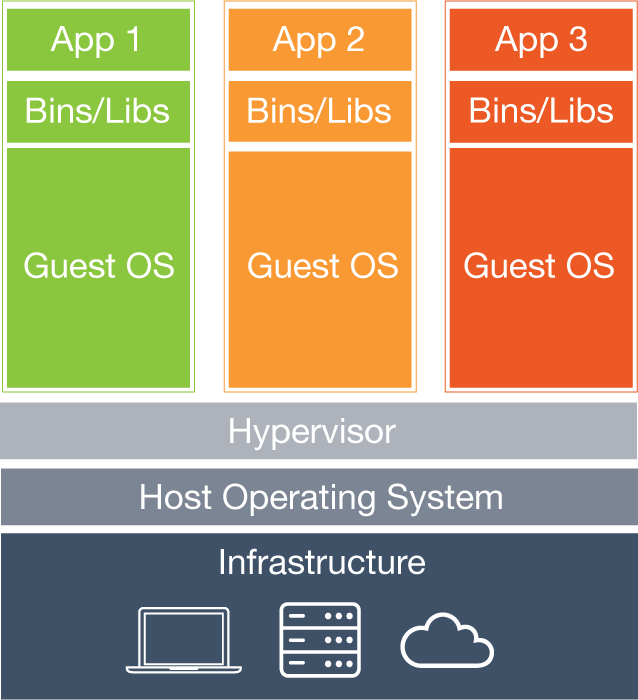
\includegraphics[width=50mm,scale=1]{imagens/what-is-docker-diagram.png}
 \caption{Diagrama docker}
 \label{fig:diagram_docker}
\end{figure}

Cada máquina virtual inclui a aplicação, os binários necessários, as bibliotecas e um sistema operativo "guest" inteiro - todos podem ser dezenas de GBs.

Já os containers incluem a aplicação e todas as suas dependências, mas partilham o kernel com outros containers. Eles correm em processos isolados no espaço do utilizador (userspace) no sistema operativo do host. Eles não estão limitados a uma infraestrutura específica, correm em - containers Docker podem correr em qualquer computador ou numa infraestrutura na cloud.

\subsubsection{DockerFile > Image > Container}

Uma imagem docker contém todos os pacotes necessários pré-instalados o que é diferente de uma imagem de uma máquina Ubuntu.

Quando a imagem está pronta é possível correr a mesma, tendo assim um container.

O bom da partilha de imagens é que, por exemplo, uma equipa pode criar o seu ambiente de desenvolvimento, com a mesma versão do Python, o mesmo Django e o mesmo PyCharm com todas as configurações pré-configuradas.

\subsubsection{Limitações}

\textbf{Limite de CPU}

\begin{figure}[!htb]
\center
 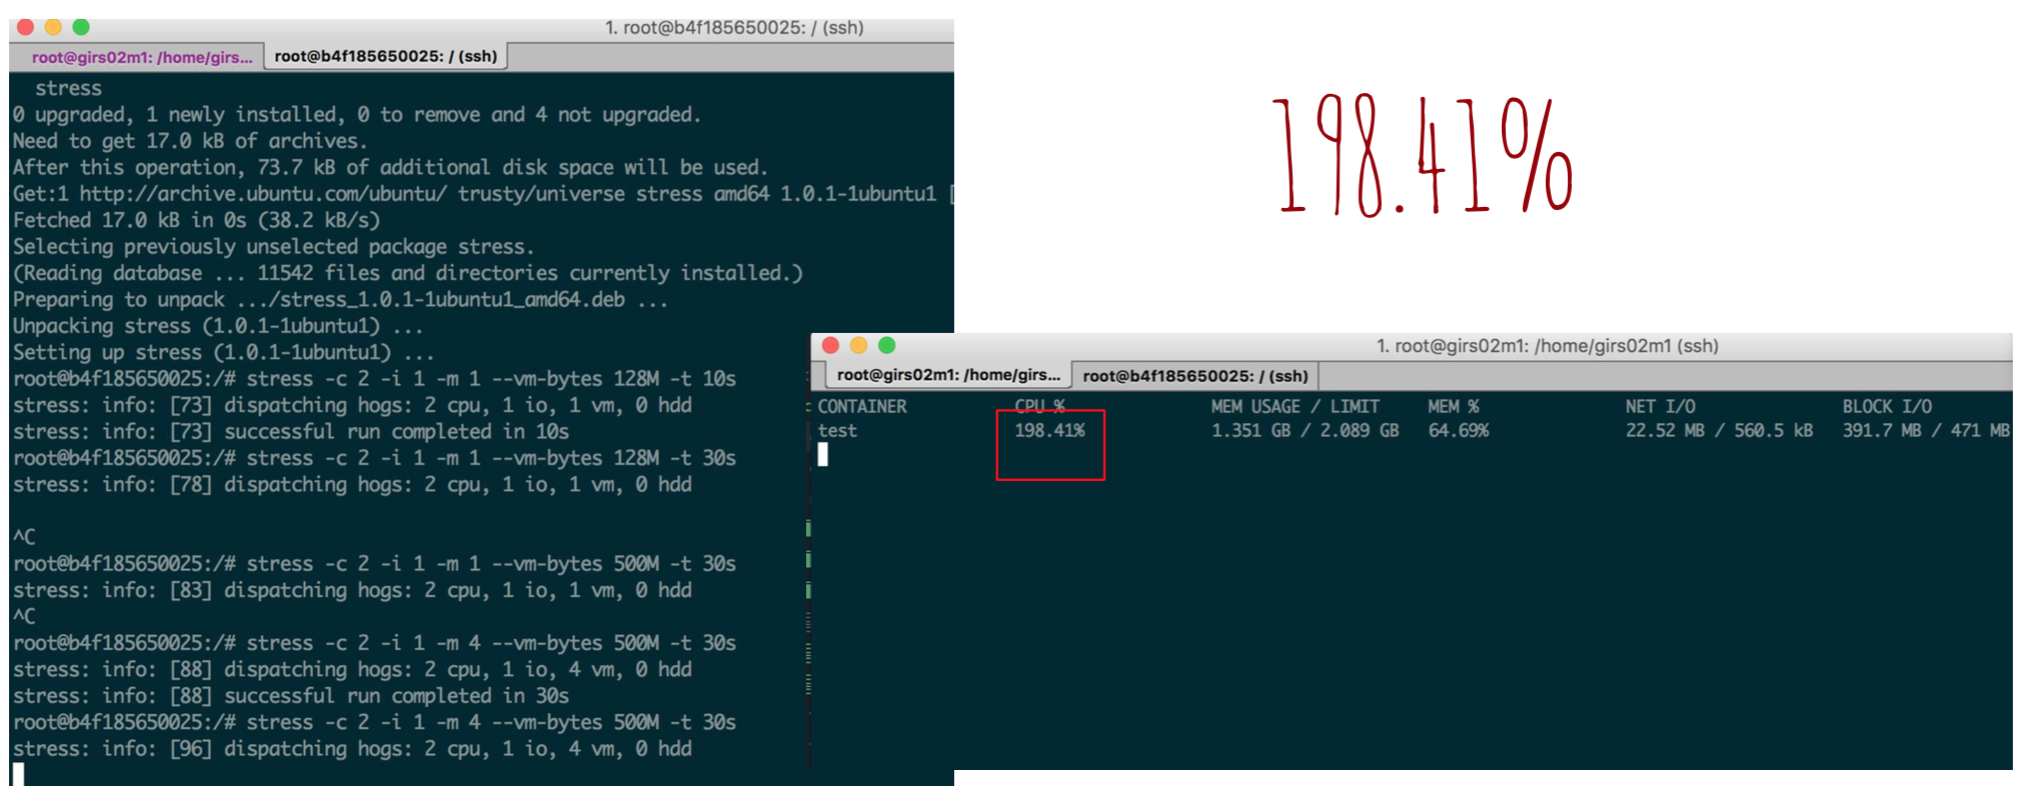
\includegraphics[width=100mm,scale=1]{imagens/cpu_limit_198.png}
 \caption{Limite de CPU 198\%}
 \label{fig:cpu_limit_198}
\end{figure}

\begin{figure}[!htb]
\center
 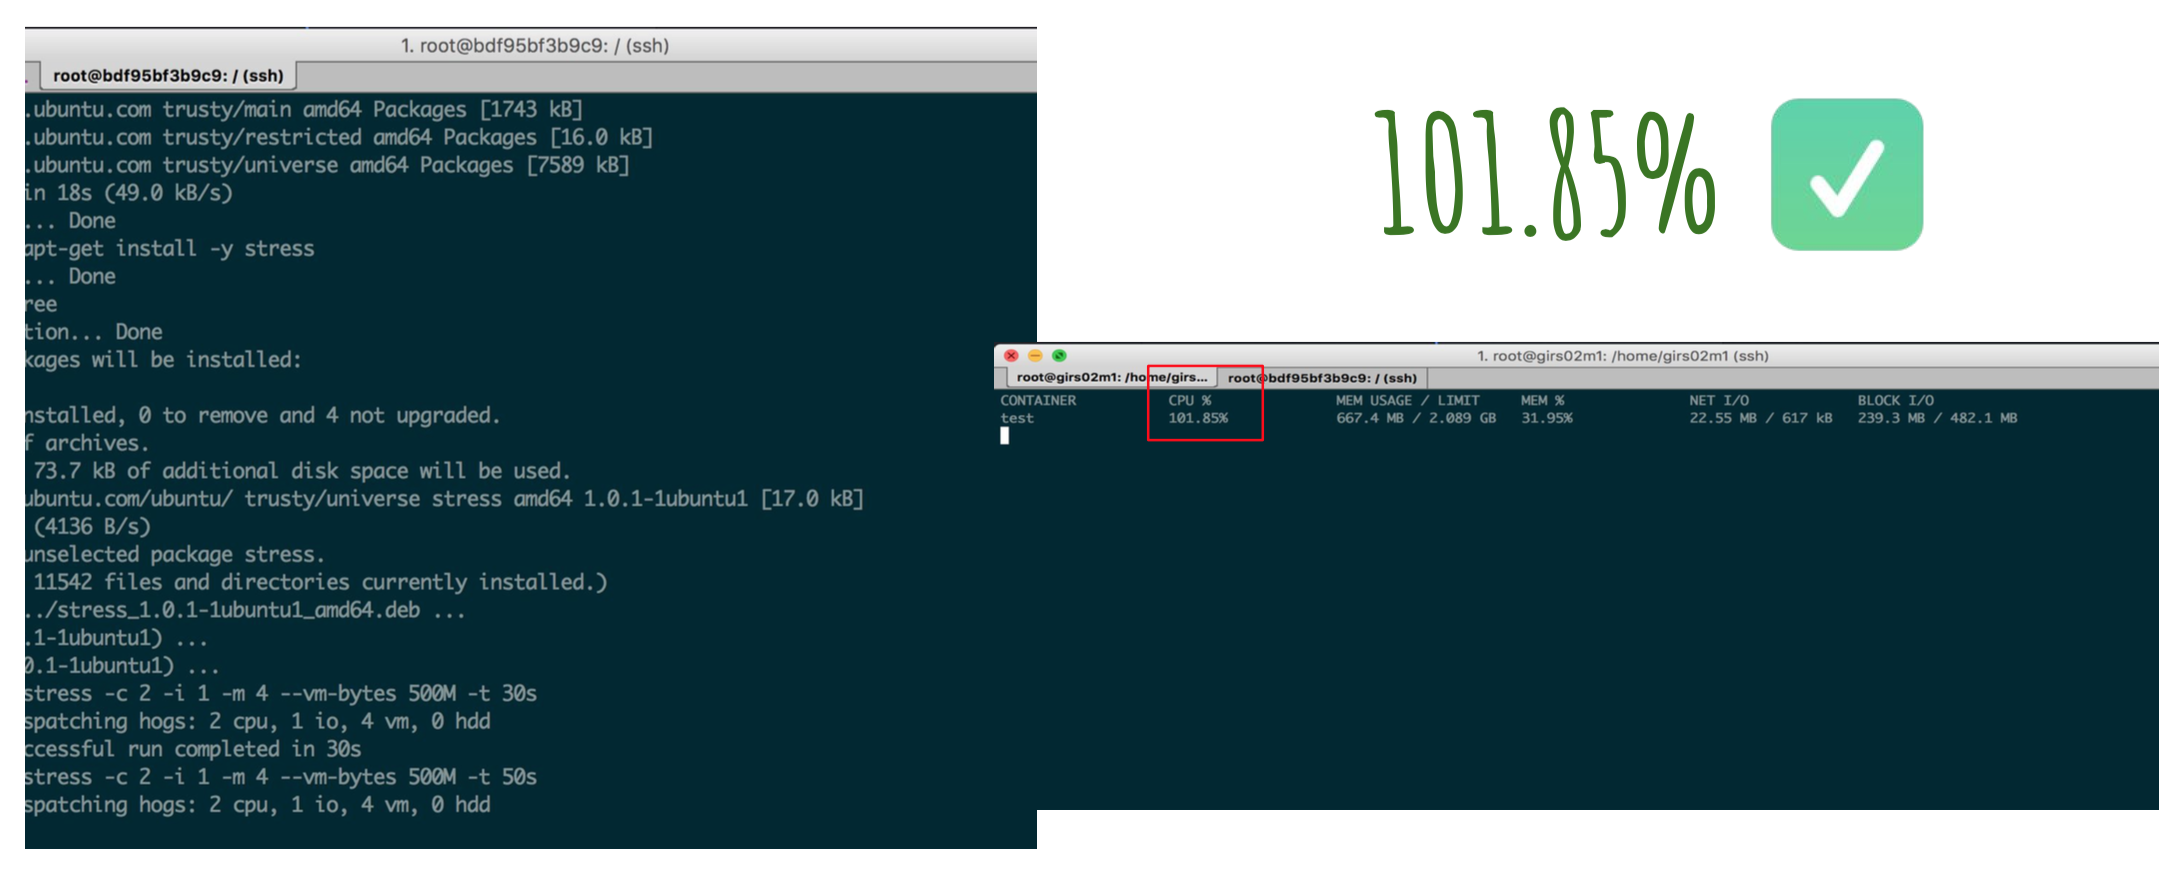
\includegraphics[width=100mm,scale=1]{imagens/cpu_limit_101.png}
 \caption{Limite de CPU 101\%}
 \label{fig:cpu_limit_101}
\end{figure}

Na primeira figura, não tem limite de CPU, por isso enchemos 198.41\% do CPU. Na segunda figura, com o limite de CPU, enchemos apenas 101.85\%, sendo assim, o limite de CPU funciona.

\textbf{Limite de RAM}

\begin{figure}[!htb]
\center
 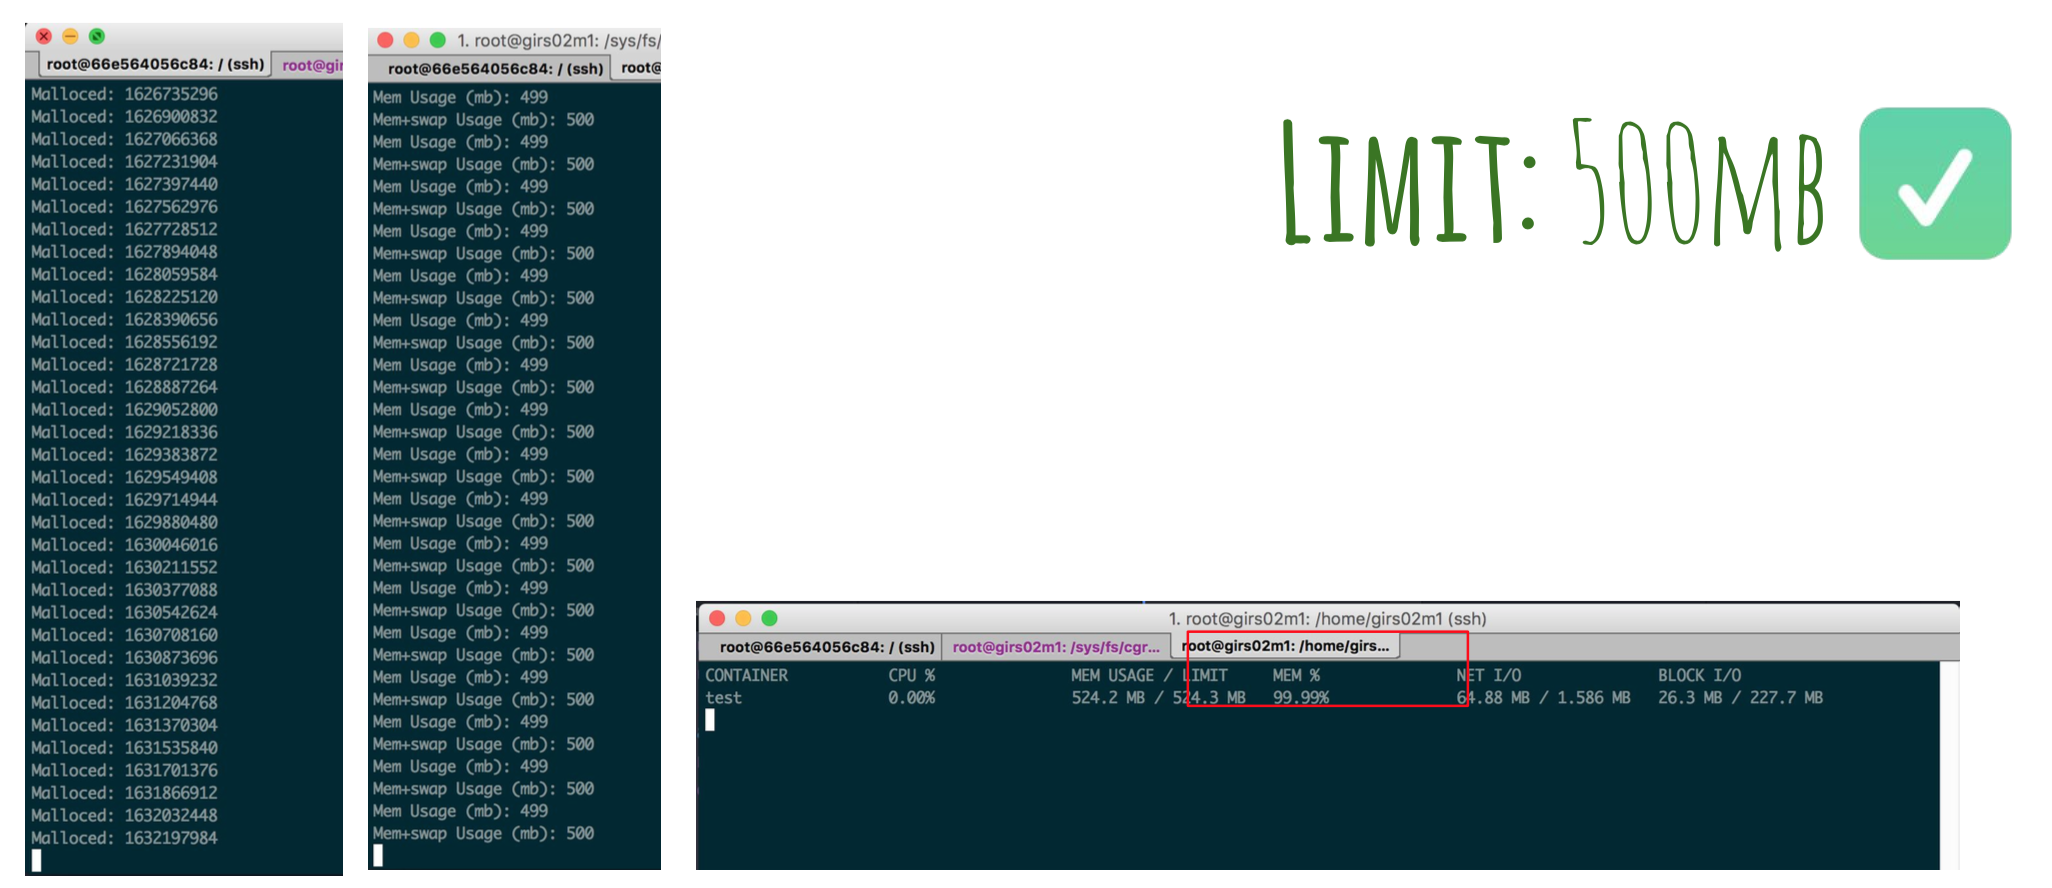
\includegraphics[width=100mm,scale=1]{imagens/memory_500.png}
 \caption{500 RAM}
 \label{fig:memory_500}
\end{figure}

Com o limite de memória RAM, também foi possível 500 MB.

\textbf{GeekBench}

\begin{figure}[!htb]
\center
 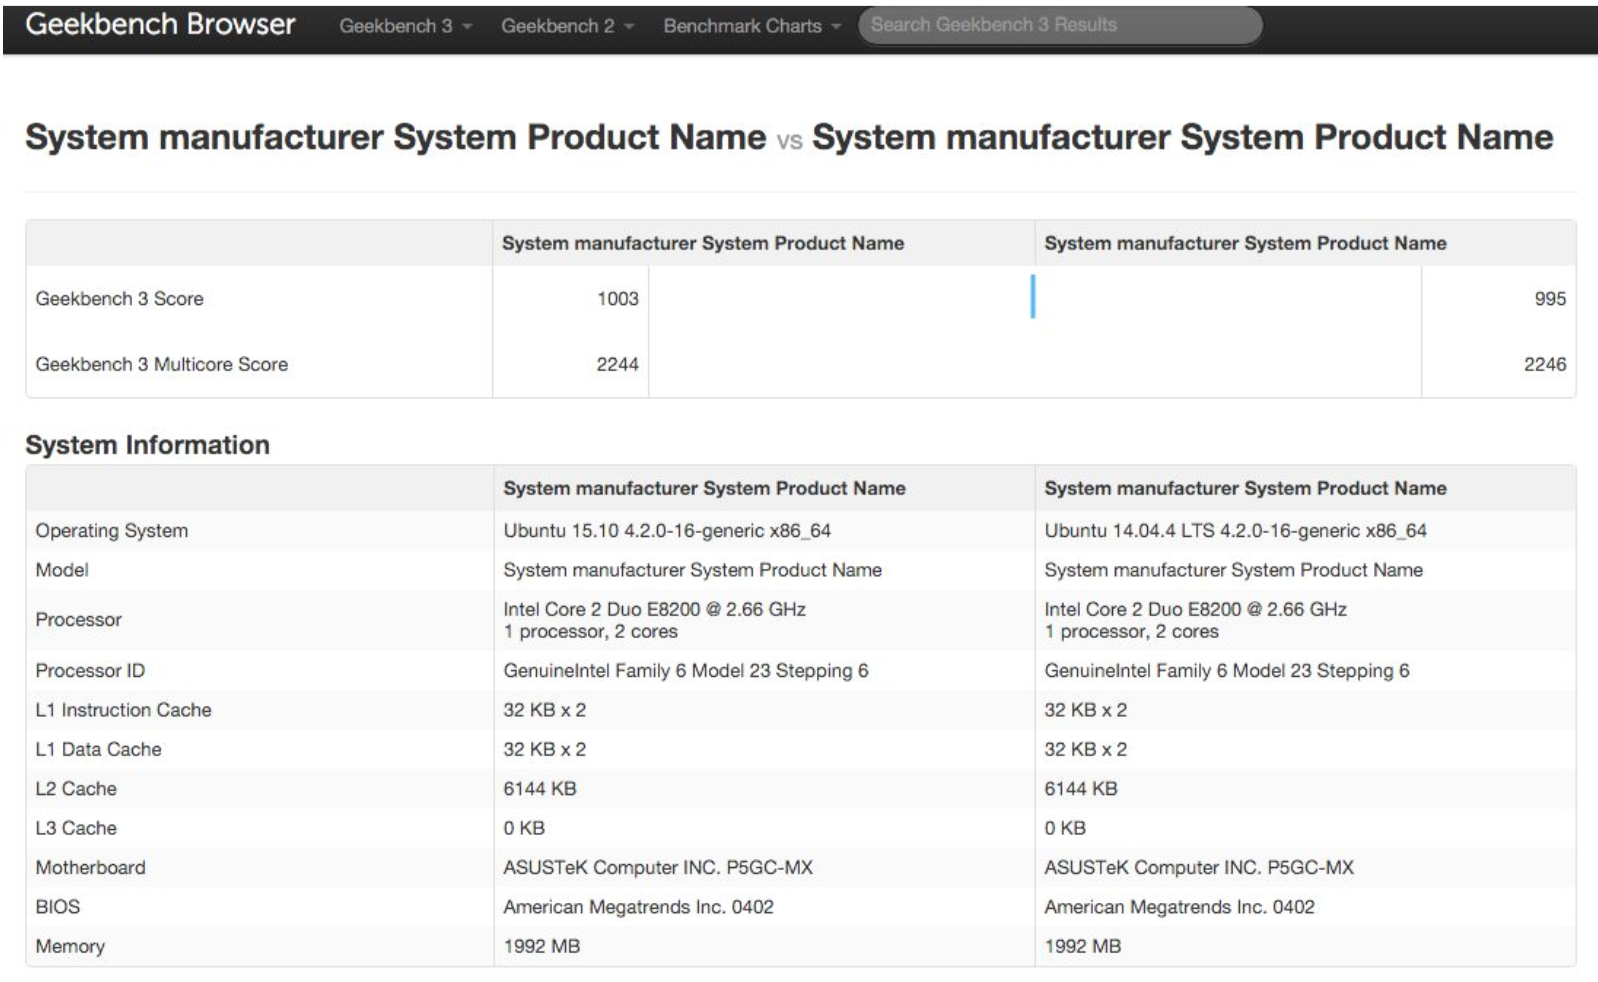
\includegraphics[width=100mm,scale=1]{imagens/geekbench.png}
 \caption{GeekBench, Host vs Container}
 \label{fig:geekbench}
\end{figure}

A comparação entre os resultados do container e do host são praticamente idênticos.

\subsection{Rancher}

Rancher é uma plataforma para gestão de vários nós que têm um docker machine. Dá a possibilidade de adicionar nós que estejam alojados ou localmente, ou na Amazon Web Services, ou na DigitalOcean, entre outras.

\begin{figure}[!htb]
\center
 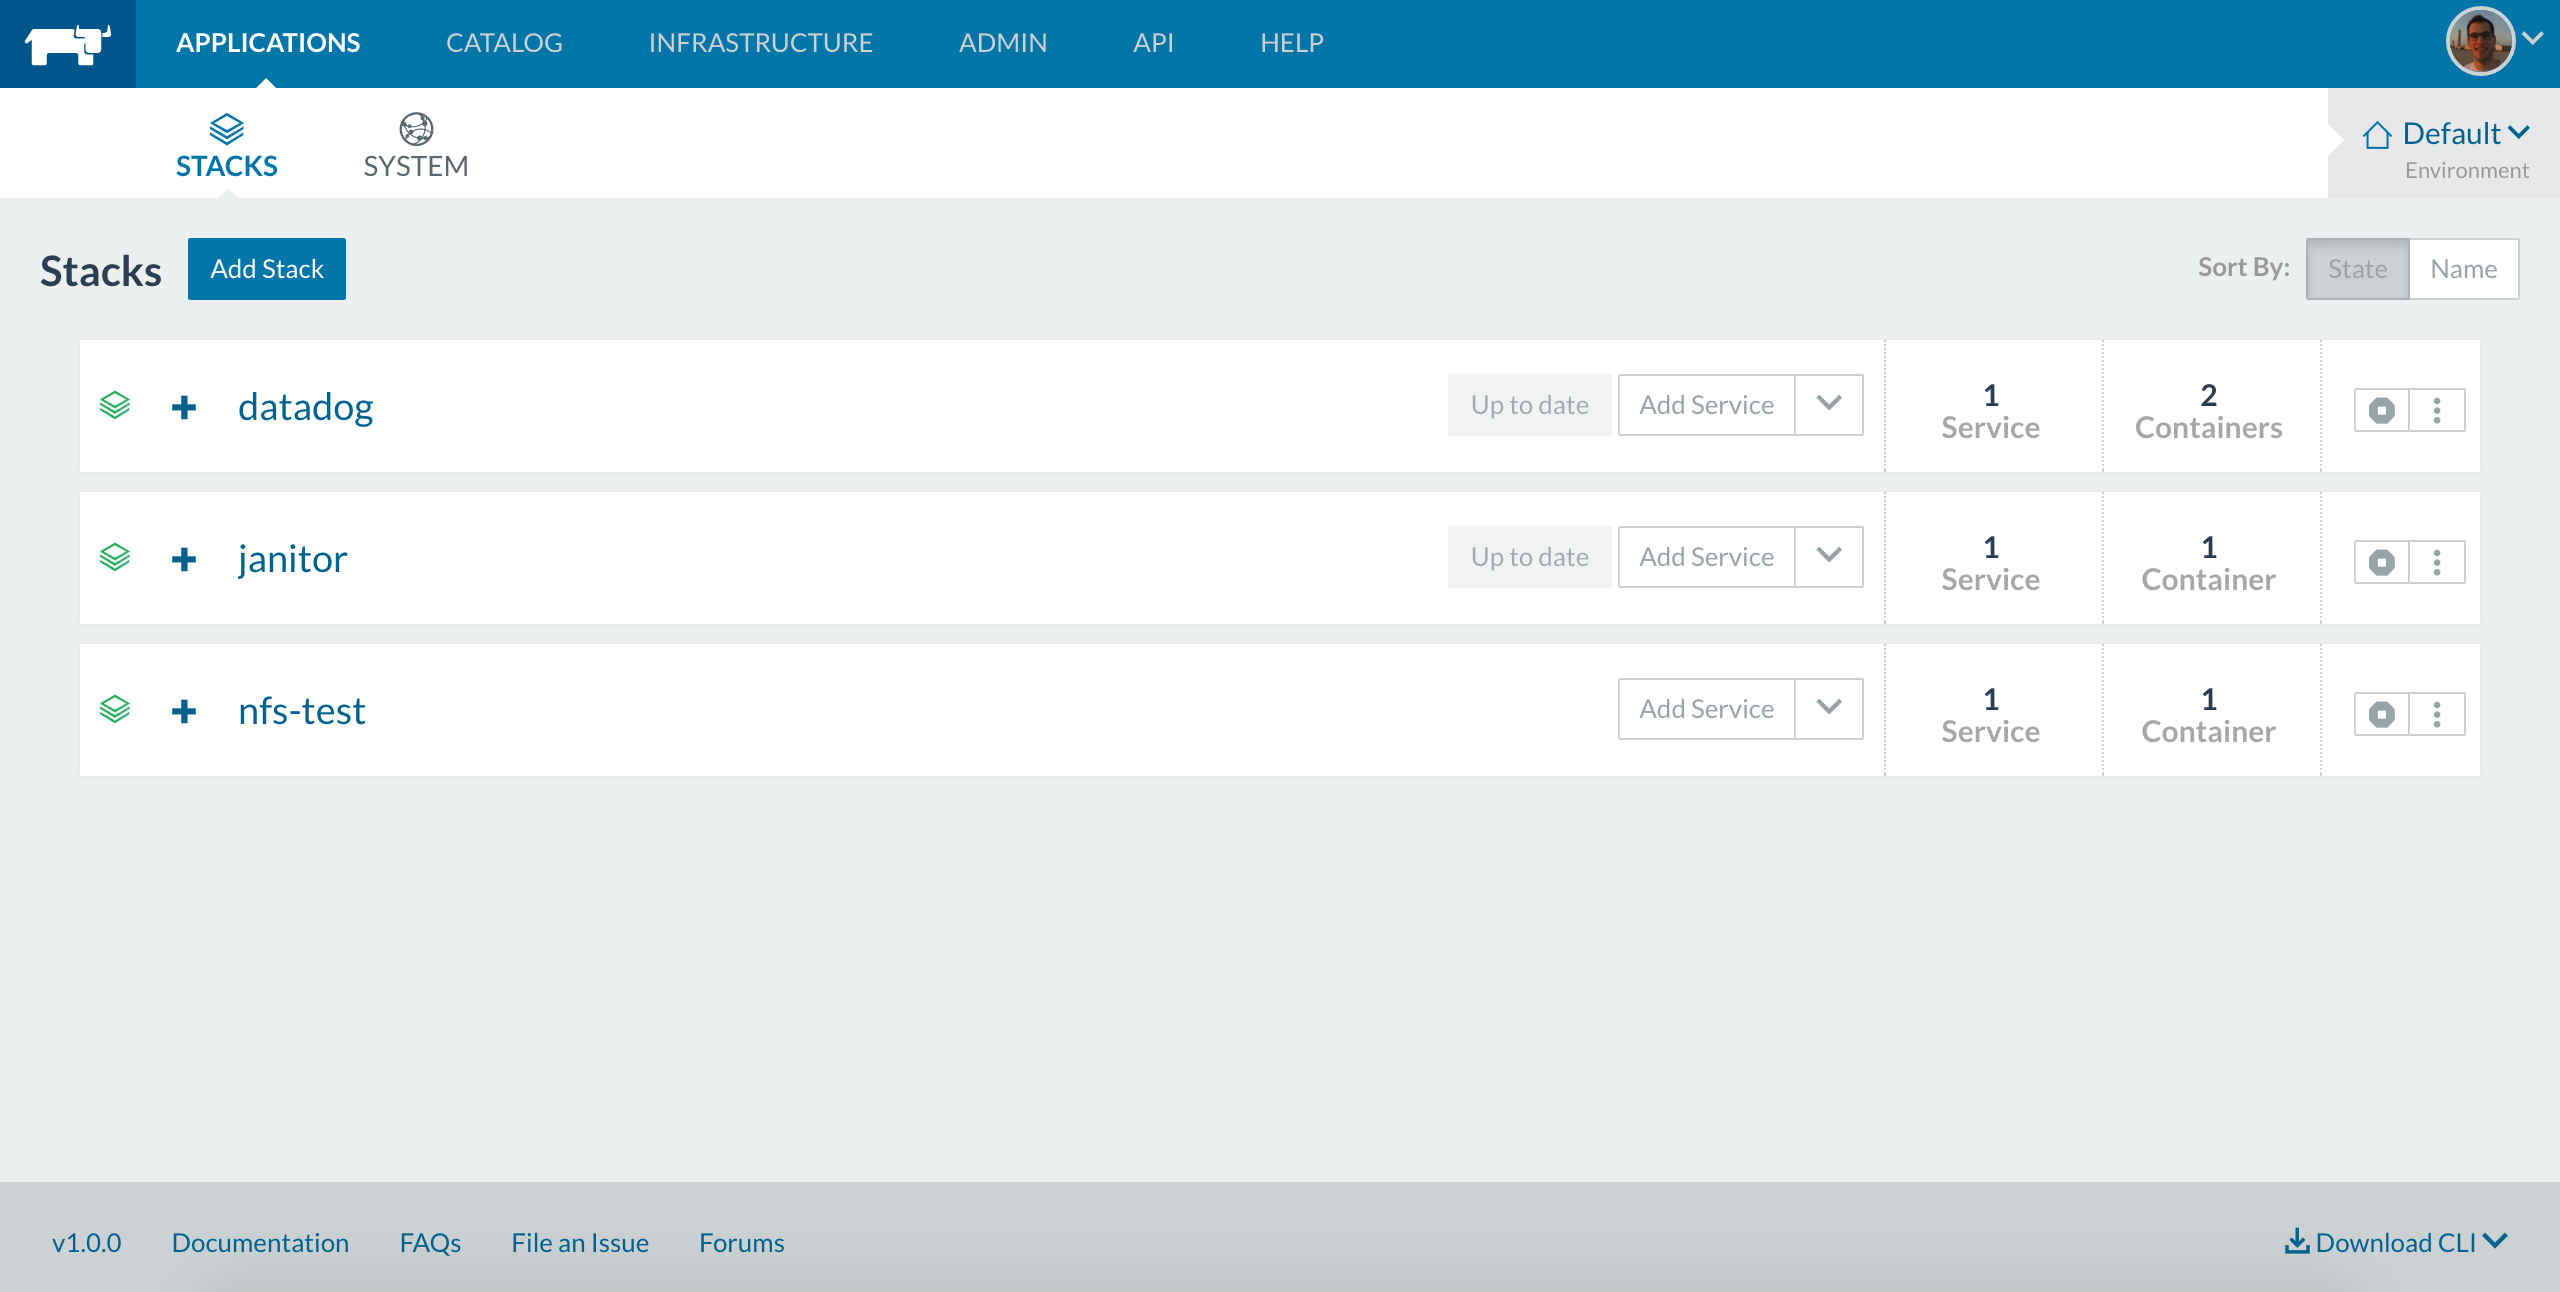
\includegraphics[width=150mm,scale=1]{imagens/rancher_intro.png}
 \caption{Página Inicial do Rancher}
 \label{fig:rancher_intro}
\end{figure}

A configuração do Rancher é muito simples. Escolhe-se uma máquina que queremos que seja o nó principal que gere todos os outros nós, sendo que este deve ter a versão mais recente do Docker instalada.

Este nó será responsável por gerir outros nós que sejam adicionados à rede do Rancher, pode ser adicionado nós dentro de um Datacenter ou em Hosting Providers externos como o DigitalOcean ou a AWS.

Para autenticação no Rancher, está disponível várias hipóteses, GitHub, LDAP ou Basic Authentication.

Na página inicial, é mostrada ao utilizador a lista de Stacks, sendo que estas devem-se organizar por serviço/aplicação.

\begin{figure}[!htb]
\centering
\begin{minipage}{.5\textwidth}
  \centering
  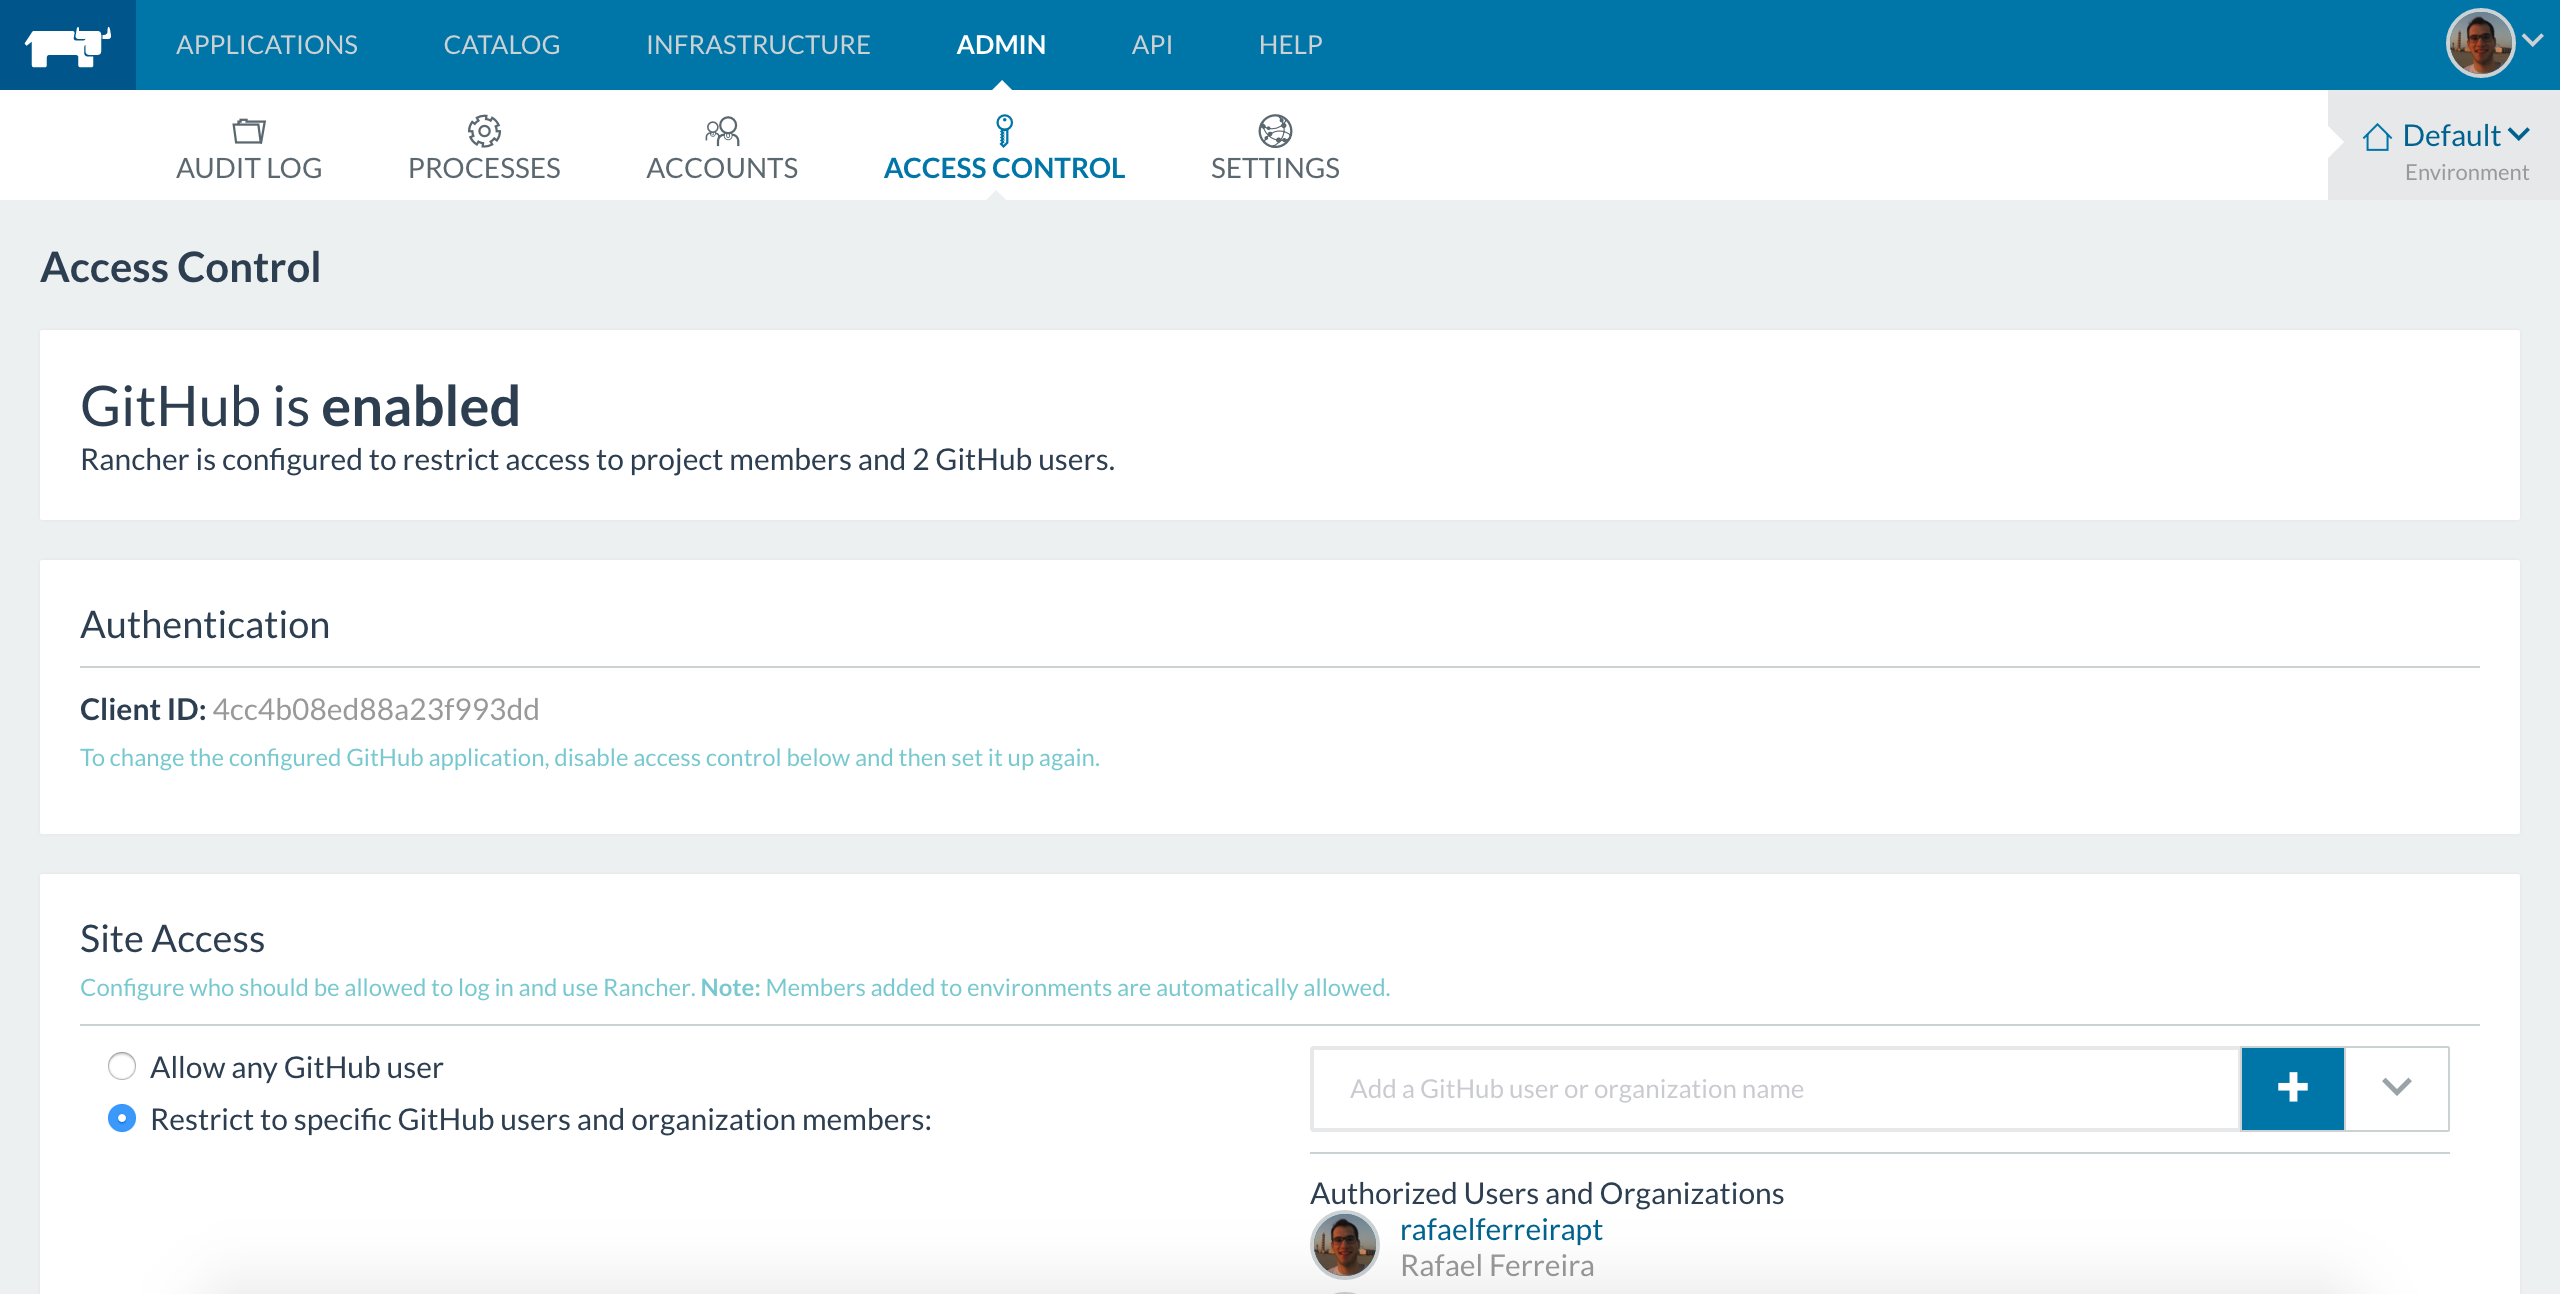
\includegraphics[width=65mm,scale=1]{imagens/access_control_github.png}
  \captionof{figure}{Access control with GitHub}
  \label{fig:access_control_github}
\end{minipage}%
\begin{minipage}{.5\textwidth}
  \centering
  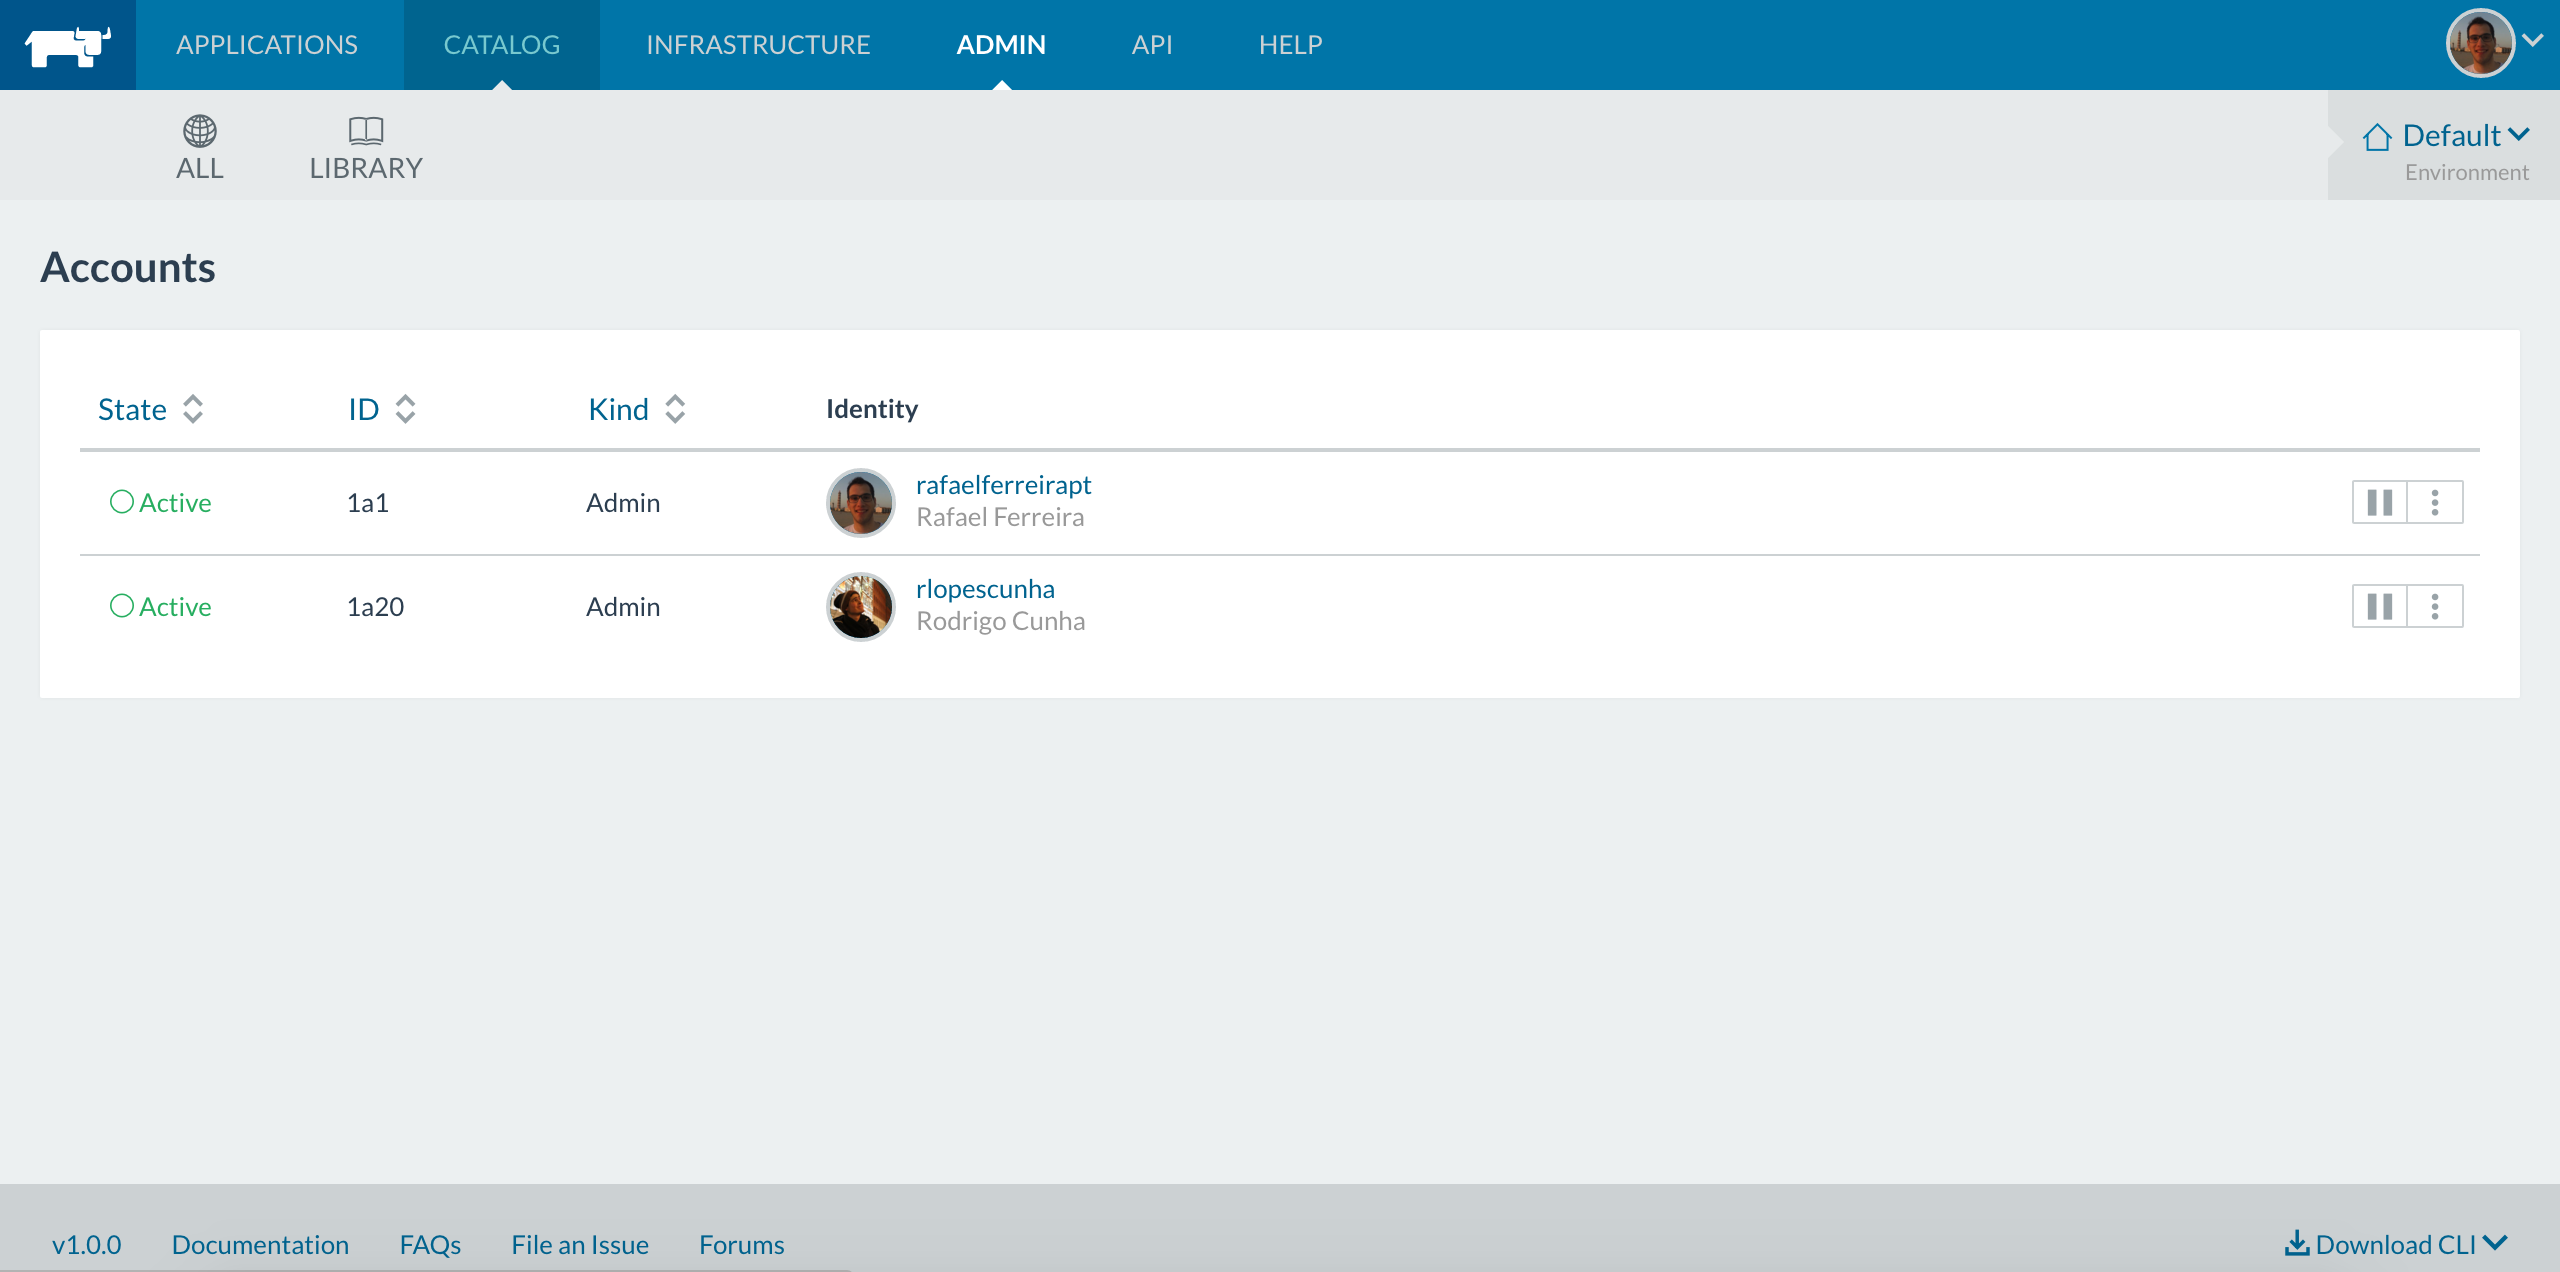
\includegraphics[width=65mm,scale=1]{imagens/admin.png}
  \captionof{figure}{Admin accounts}
  \label{fig:admin}
\end{minipage}
\end{figure}

Ainda no painel de administração, pode-se ainda ver os processos que estão a correr, ver um log de ações na administração e ainda mudar algumas configurações.

\begin{figure}[!htb]
\centering
\begin{minipage}{.5\textwidth}
  \centering
  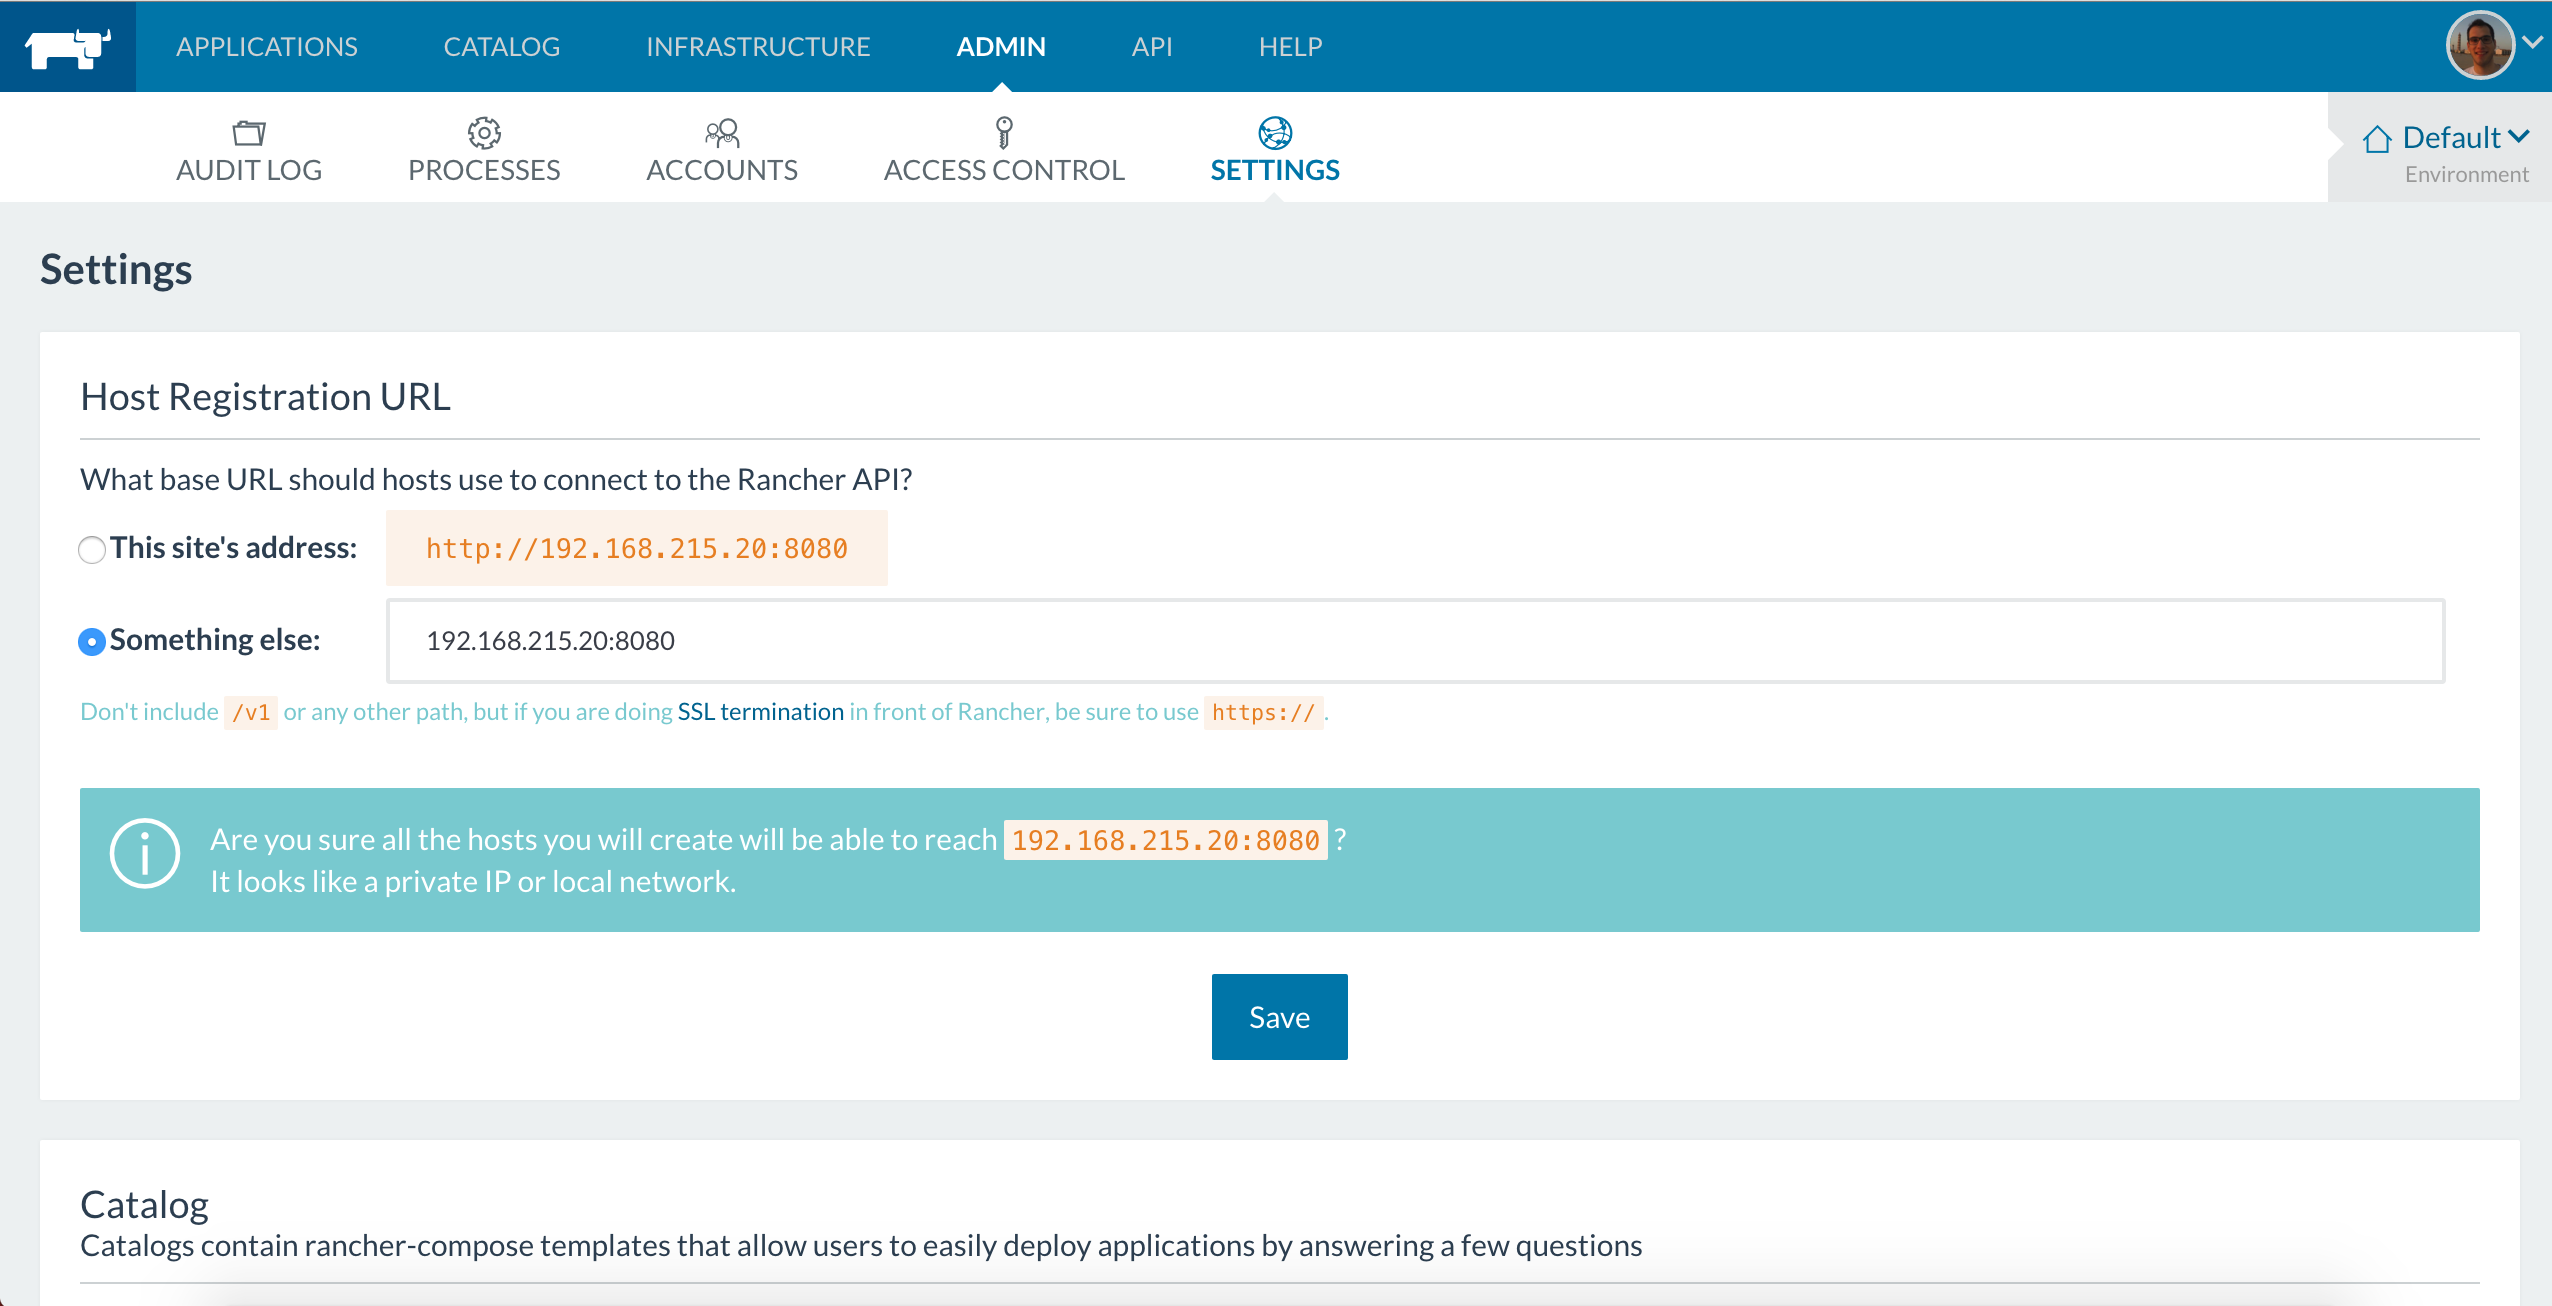
\includegraphics[width=65mm,scale=1]{imagens/settings.png}
  \captionof{figure}{Definições}
  \label{fig:settings}
\end{minipage}%
\begin{minipage}{.5\textwidth}
  \centering
  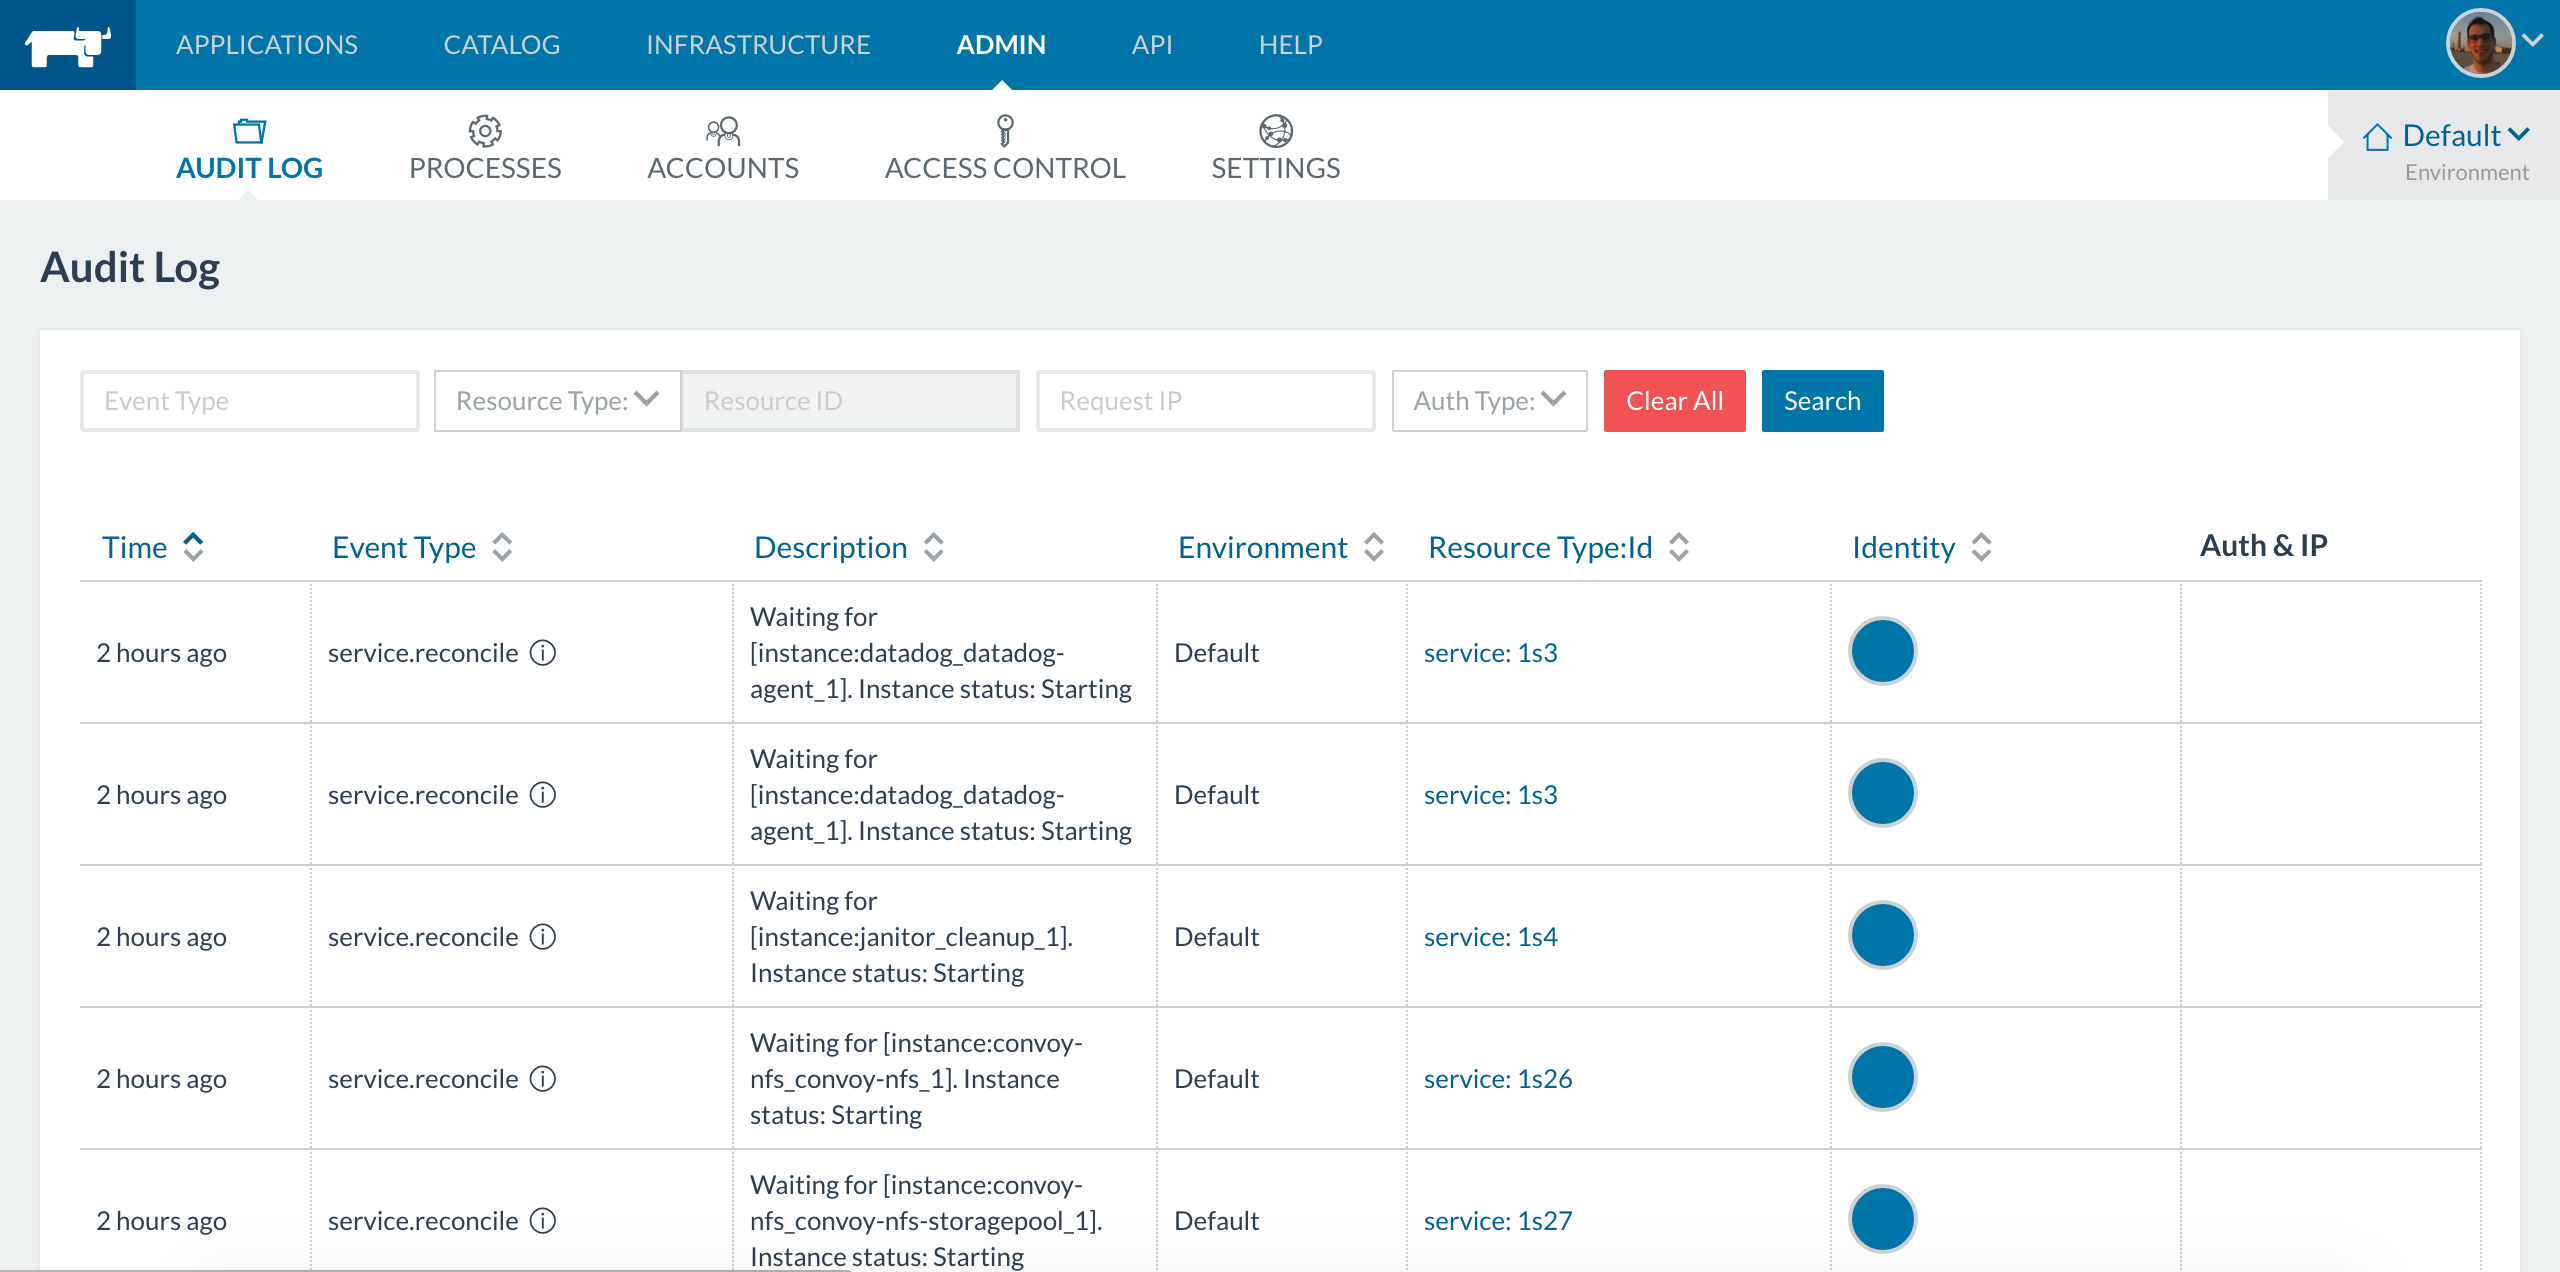
\includegraphics[width=65mm,scale=1]{imagens/audit_log.png}
  \captionof{figure}{Log de ações}
  \label{fig:audit_log}
\end{minipage}
\end{figure}

O Rancher também tem uma API para o exterior, pelo que é dito na documentação, as features são primeiro desenvolvidas para a API e só depois aparecem na interface gráfica. São também um meio de comunicação para programas que podem ser desenvolvidos posteriormente com base na API do Rancher.

\begin{figure}[!htb]
\centering
\begin{minipage}{.5\textwidth}
  \centering
  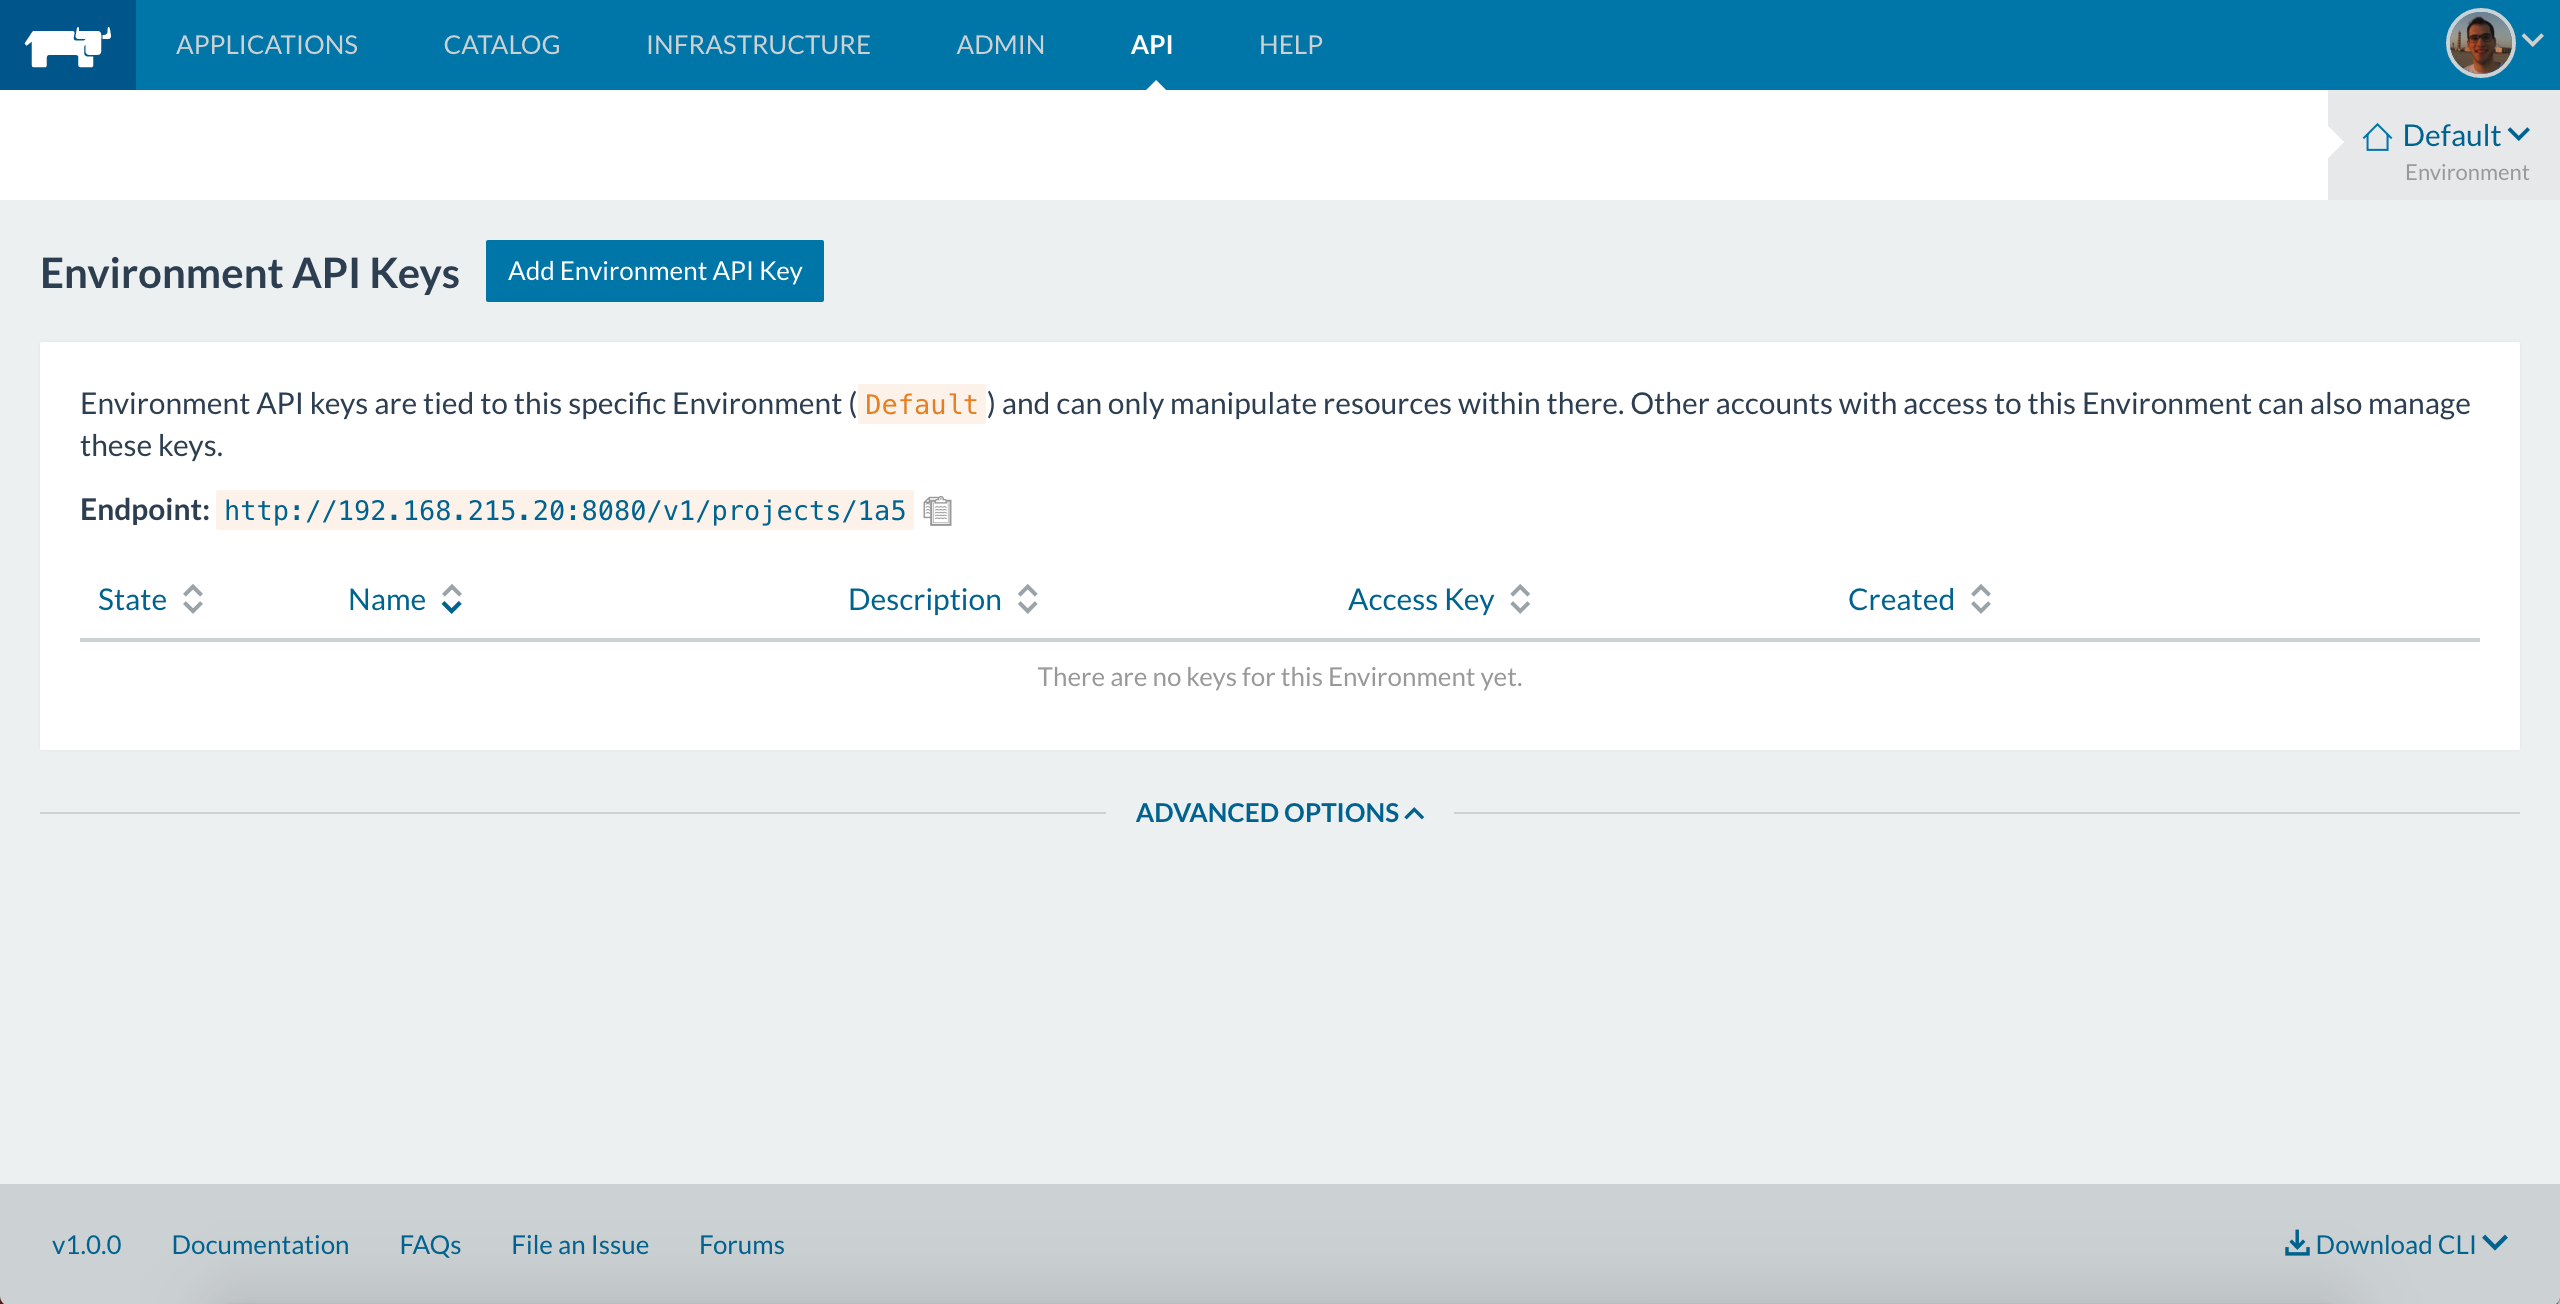
\includegraphics[width=65mm,scale=1]{imagens/api_panel.png}
  \captionof{figure}{API Rancher}
  \label{fig:api_panel}
\end{minipage}%
\begin{minipage}{.5\textwidth}
  \centering
  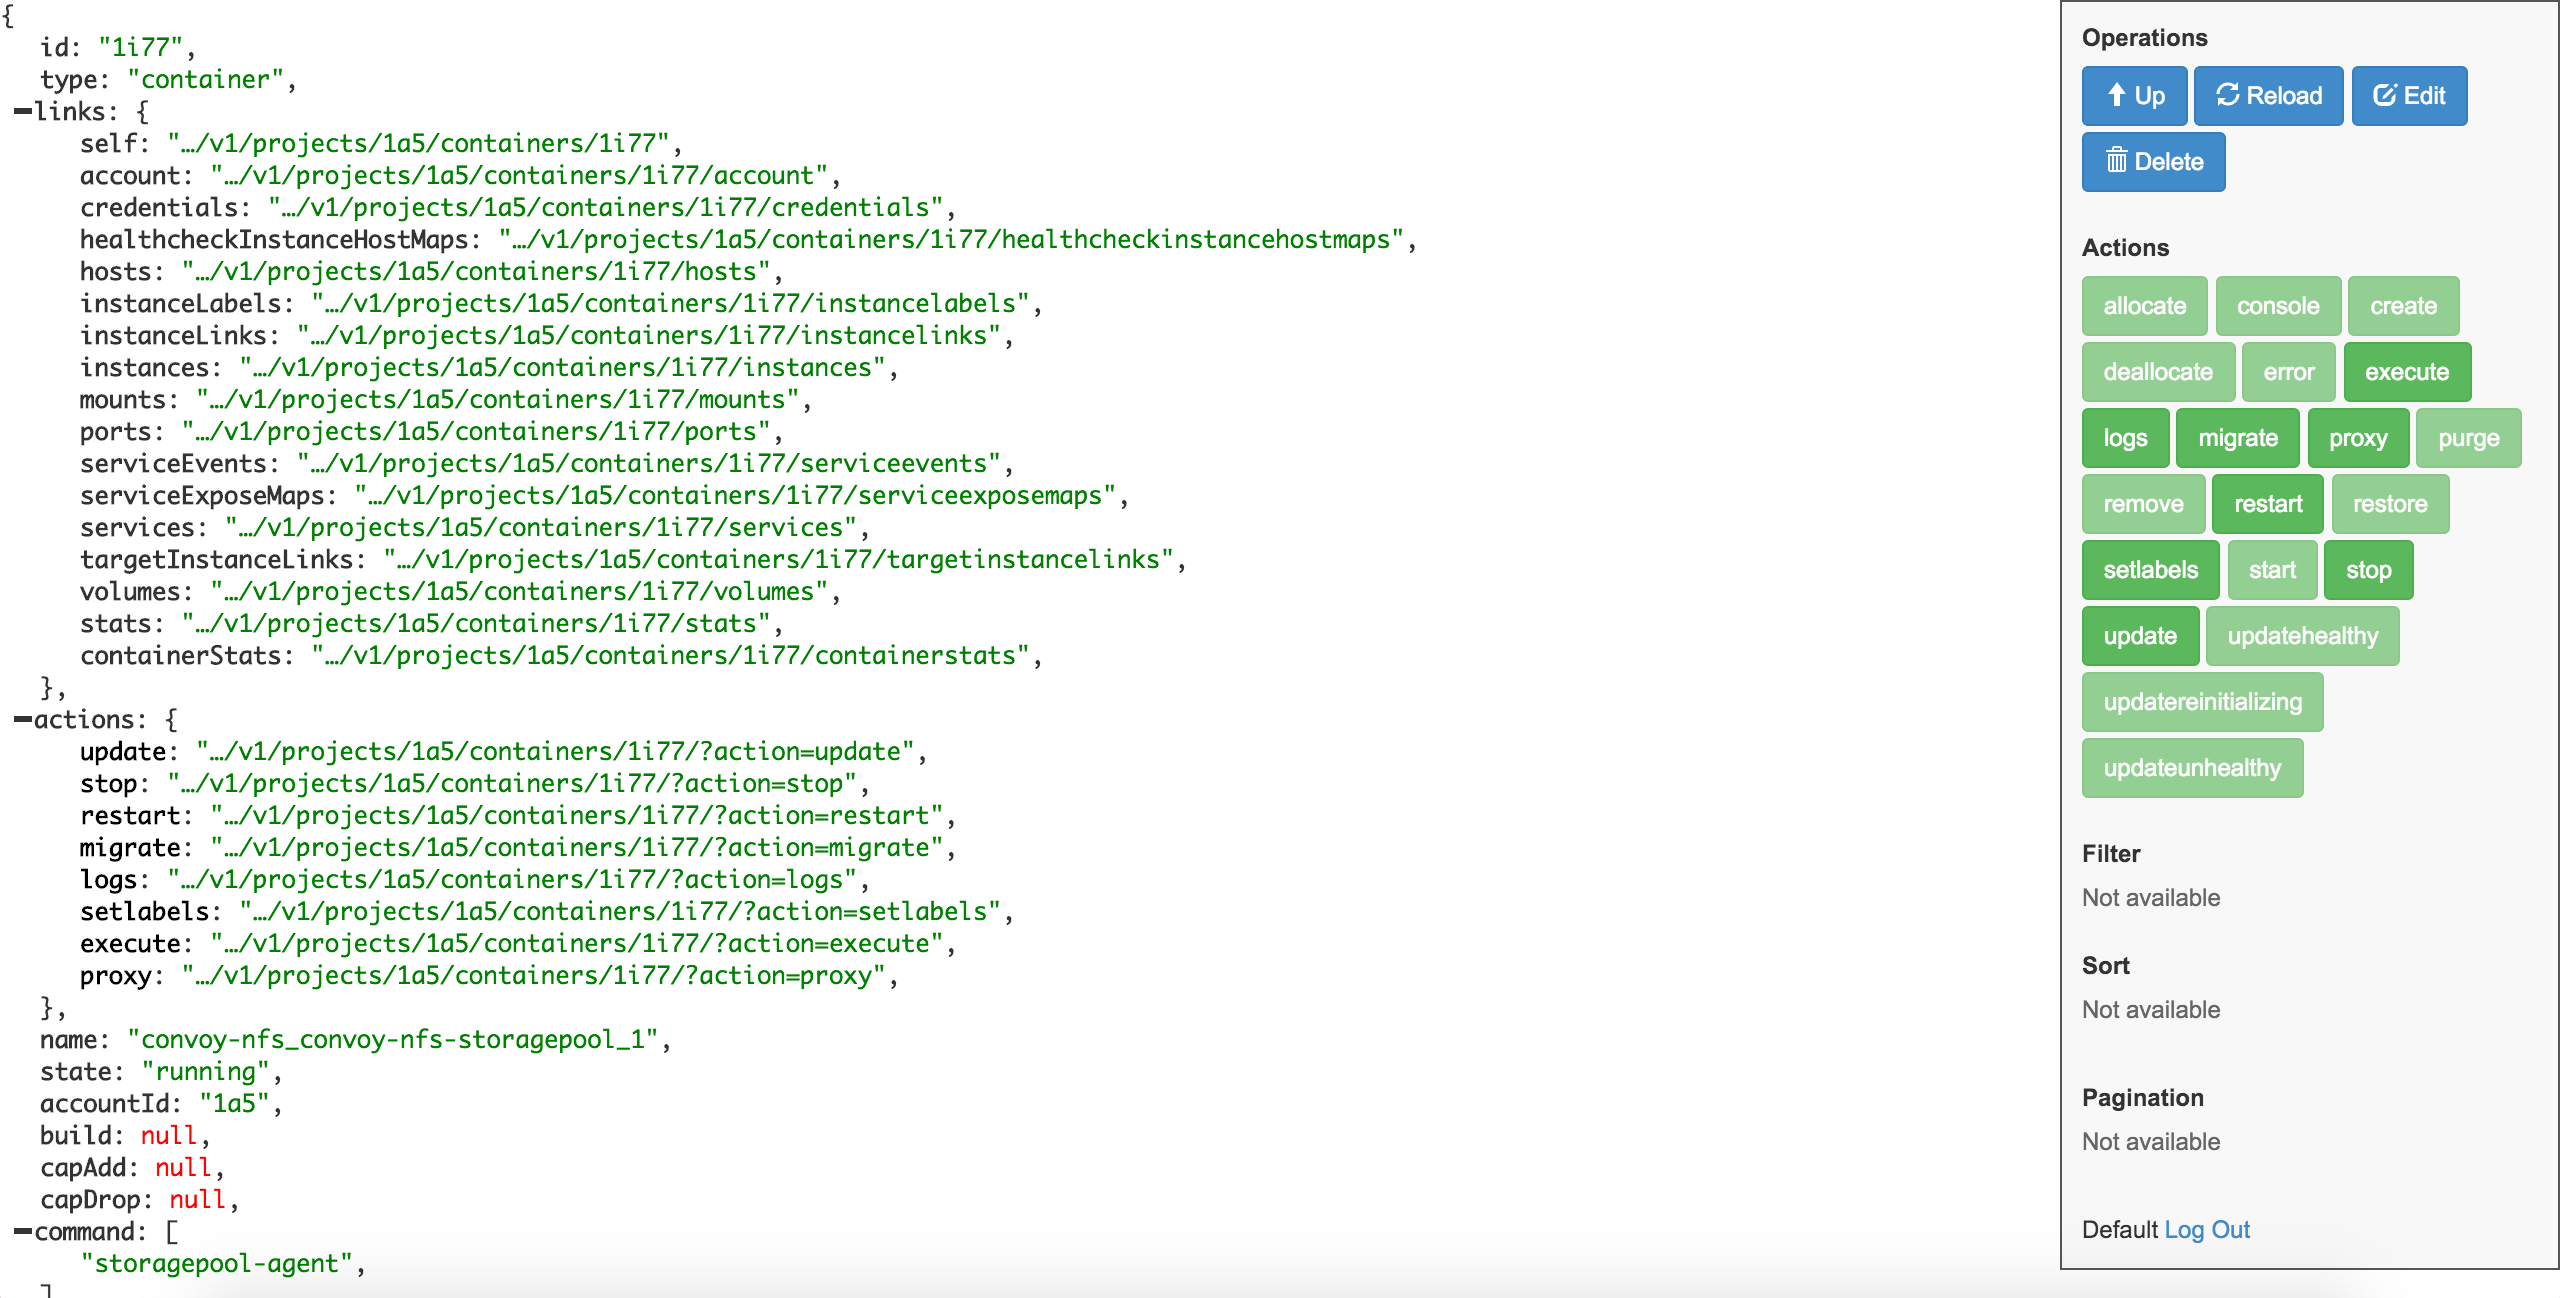
\includegraphics[width=65mm,scale=1]{imagens/api_container.png}
  \captionof{figure}{API Container}
  \label{fig:api_container}
\end{minipage}
\end{figure}

No painel da infraestrutura é possível ver os Hosts adicionados, containers ativo nos vários Hosts, Storage pools adicionados, certificados e Private Registries.

Podem ser adicionados Hosts do data center, locais ou de data centers como DigitalOcean, AWS entre outros.

Já os storage pools é possível adicionar storage com NFS.

Para gravar imagens locais, privadas, normalmente criam-se Private Registries.

\begin{figure}[!htb]
\centering
\begin{minipage}{.5\textwidth}
  \centering
  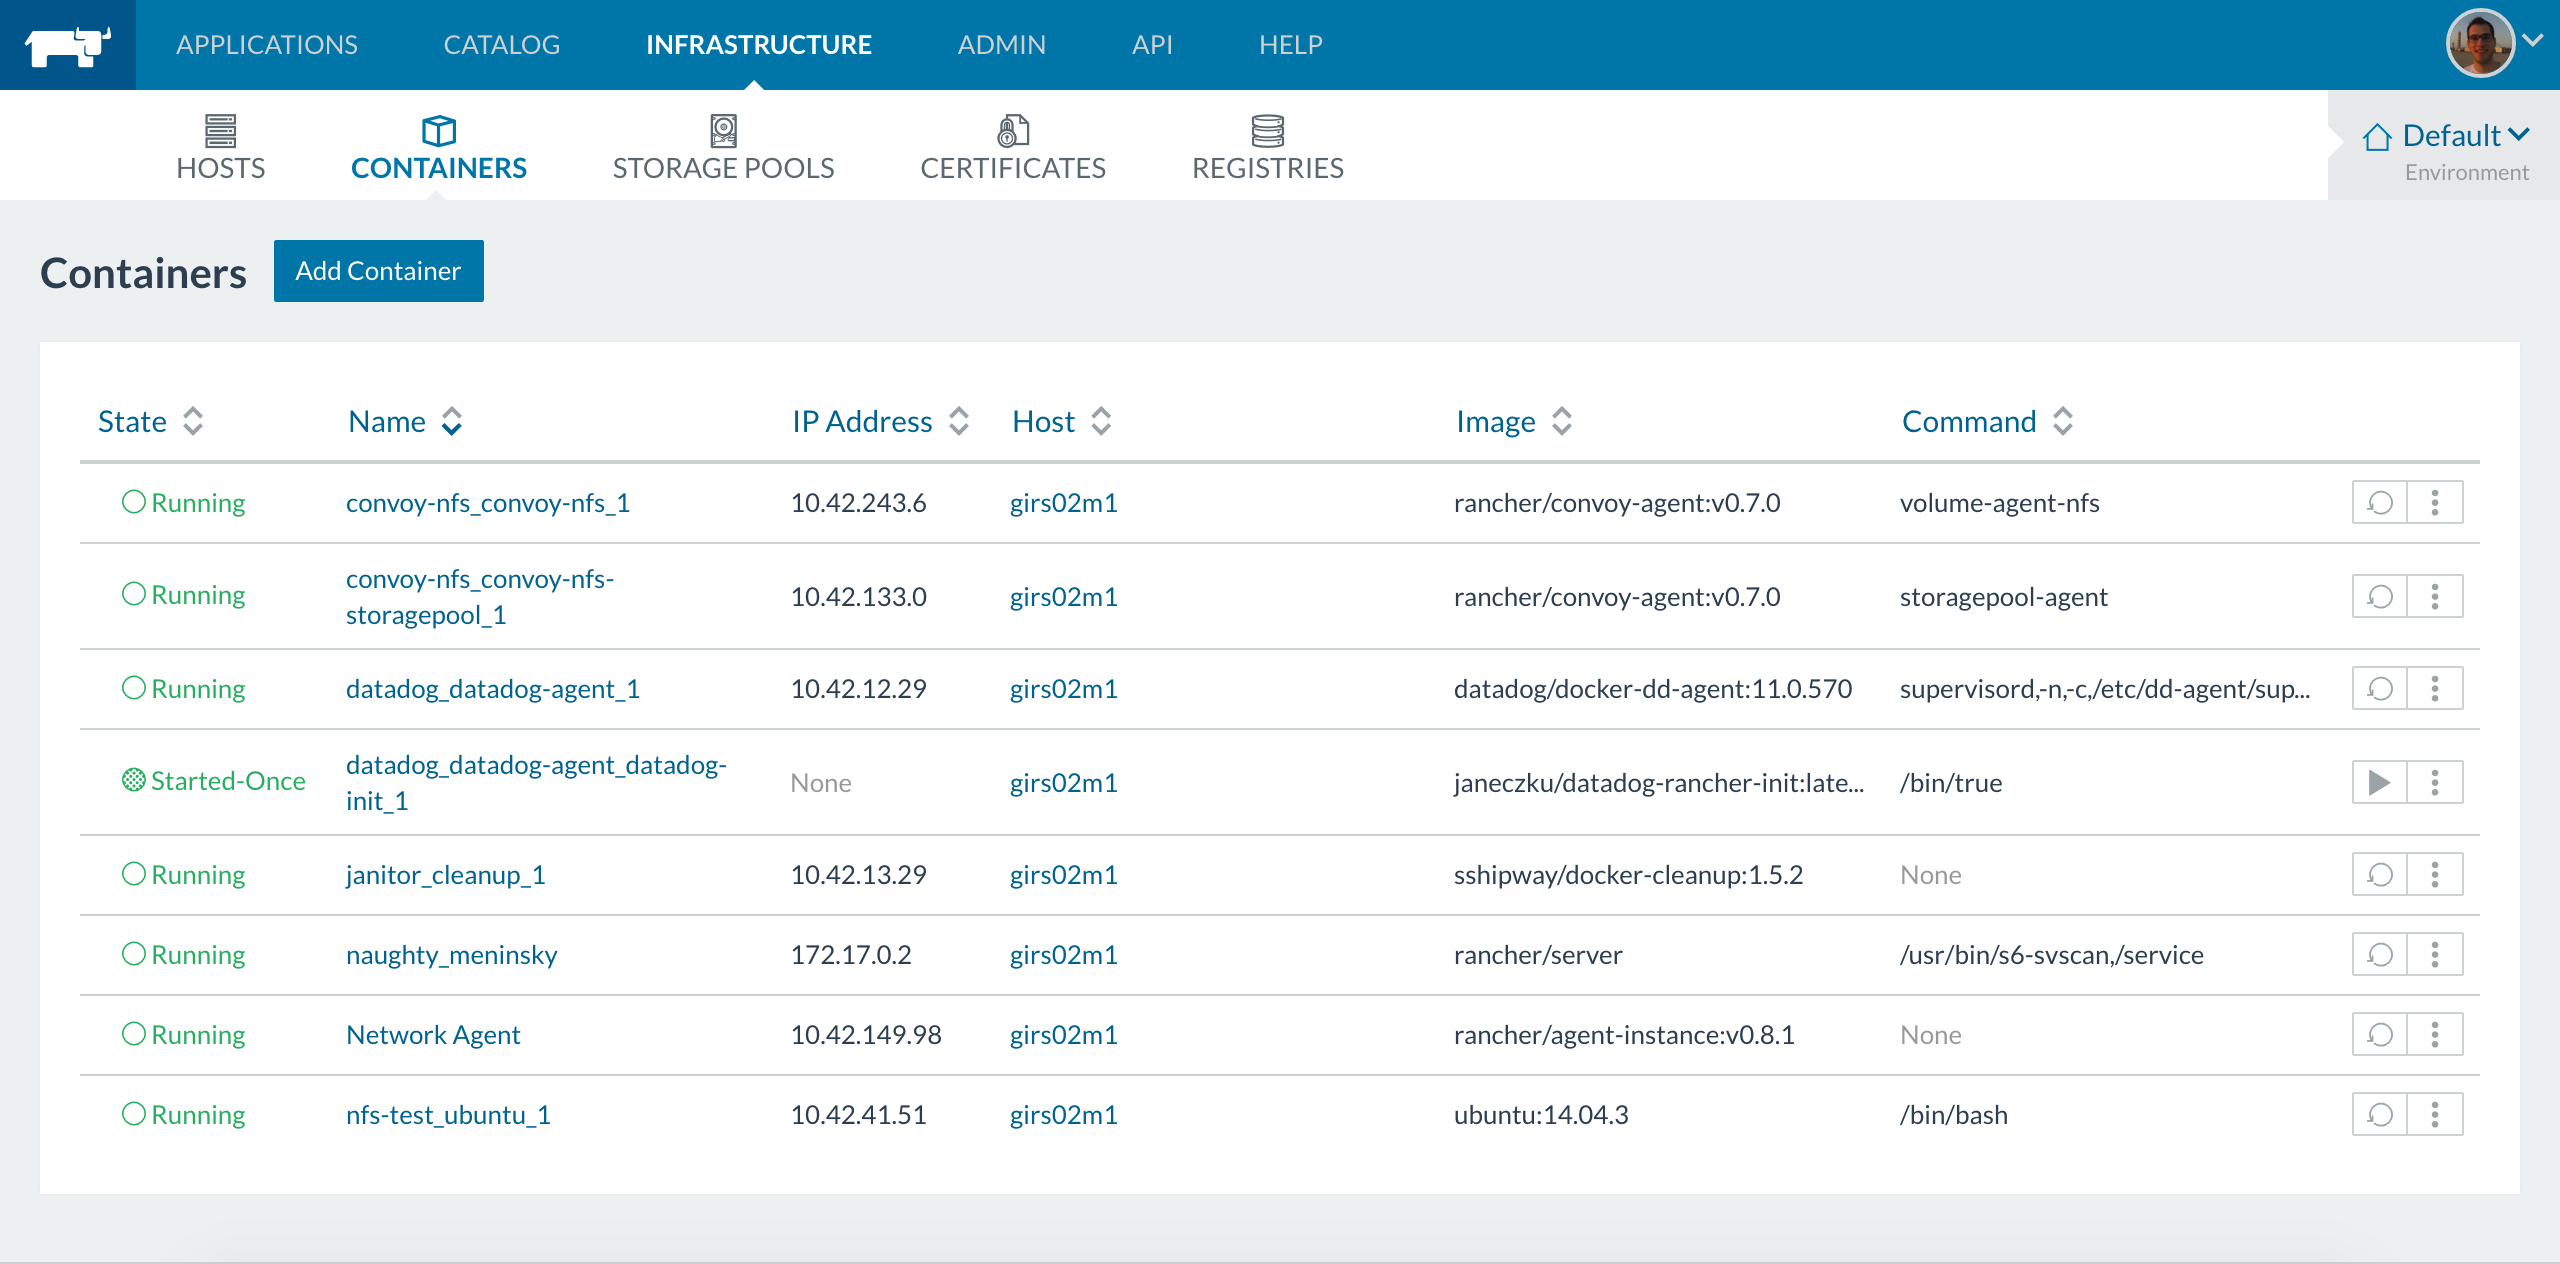
\includegraphics[width=65mm,scale=1]{imagens/containers.png}
  \captionof{figure}{Containers}
  \label{fig:containers}
\end{minipage}%
\begin{minipage}{.5\textwidth}
  \centering
  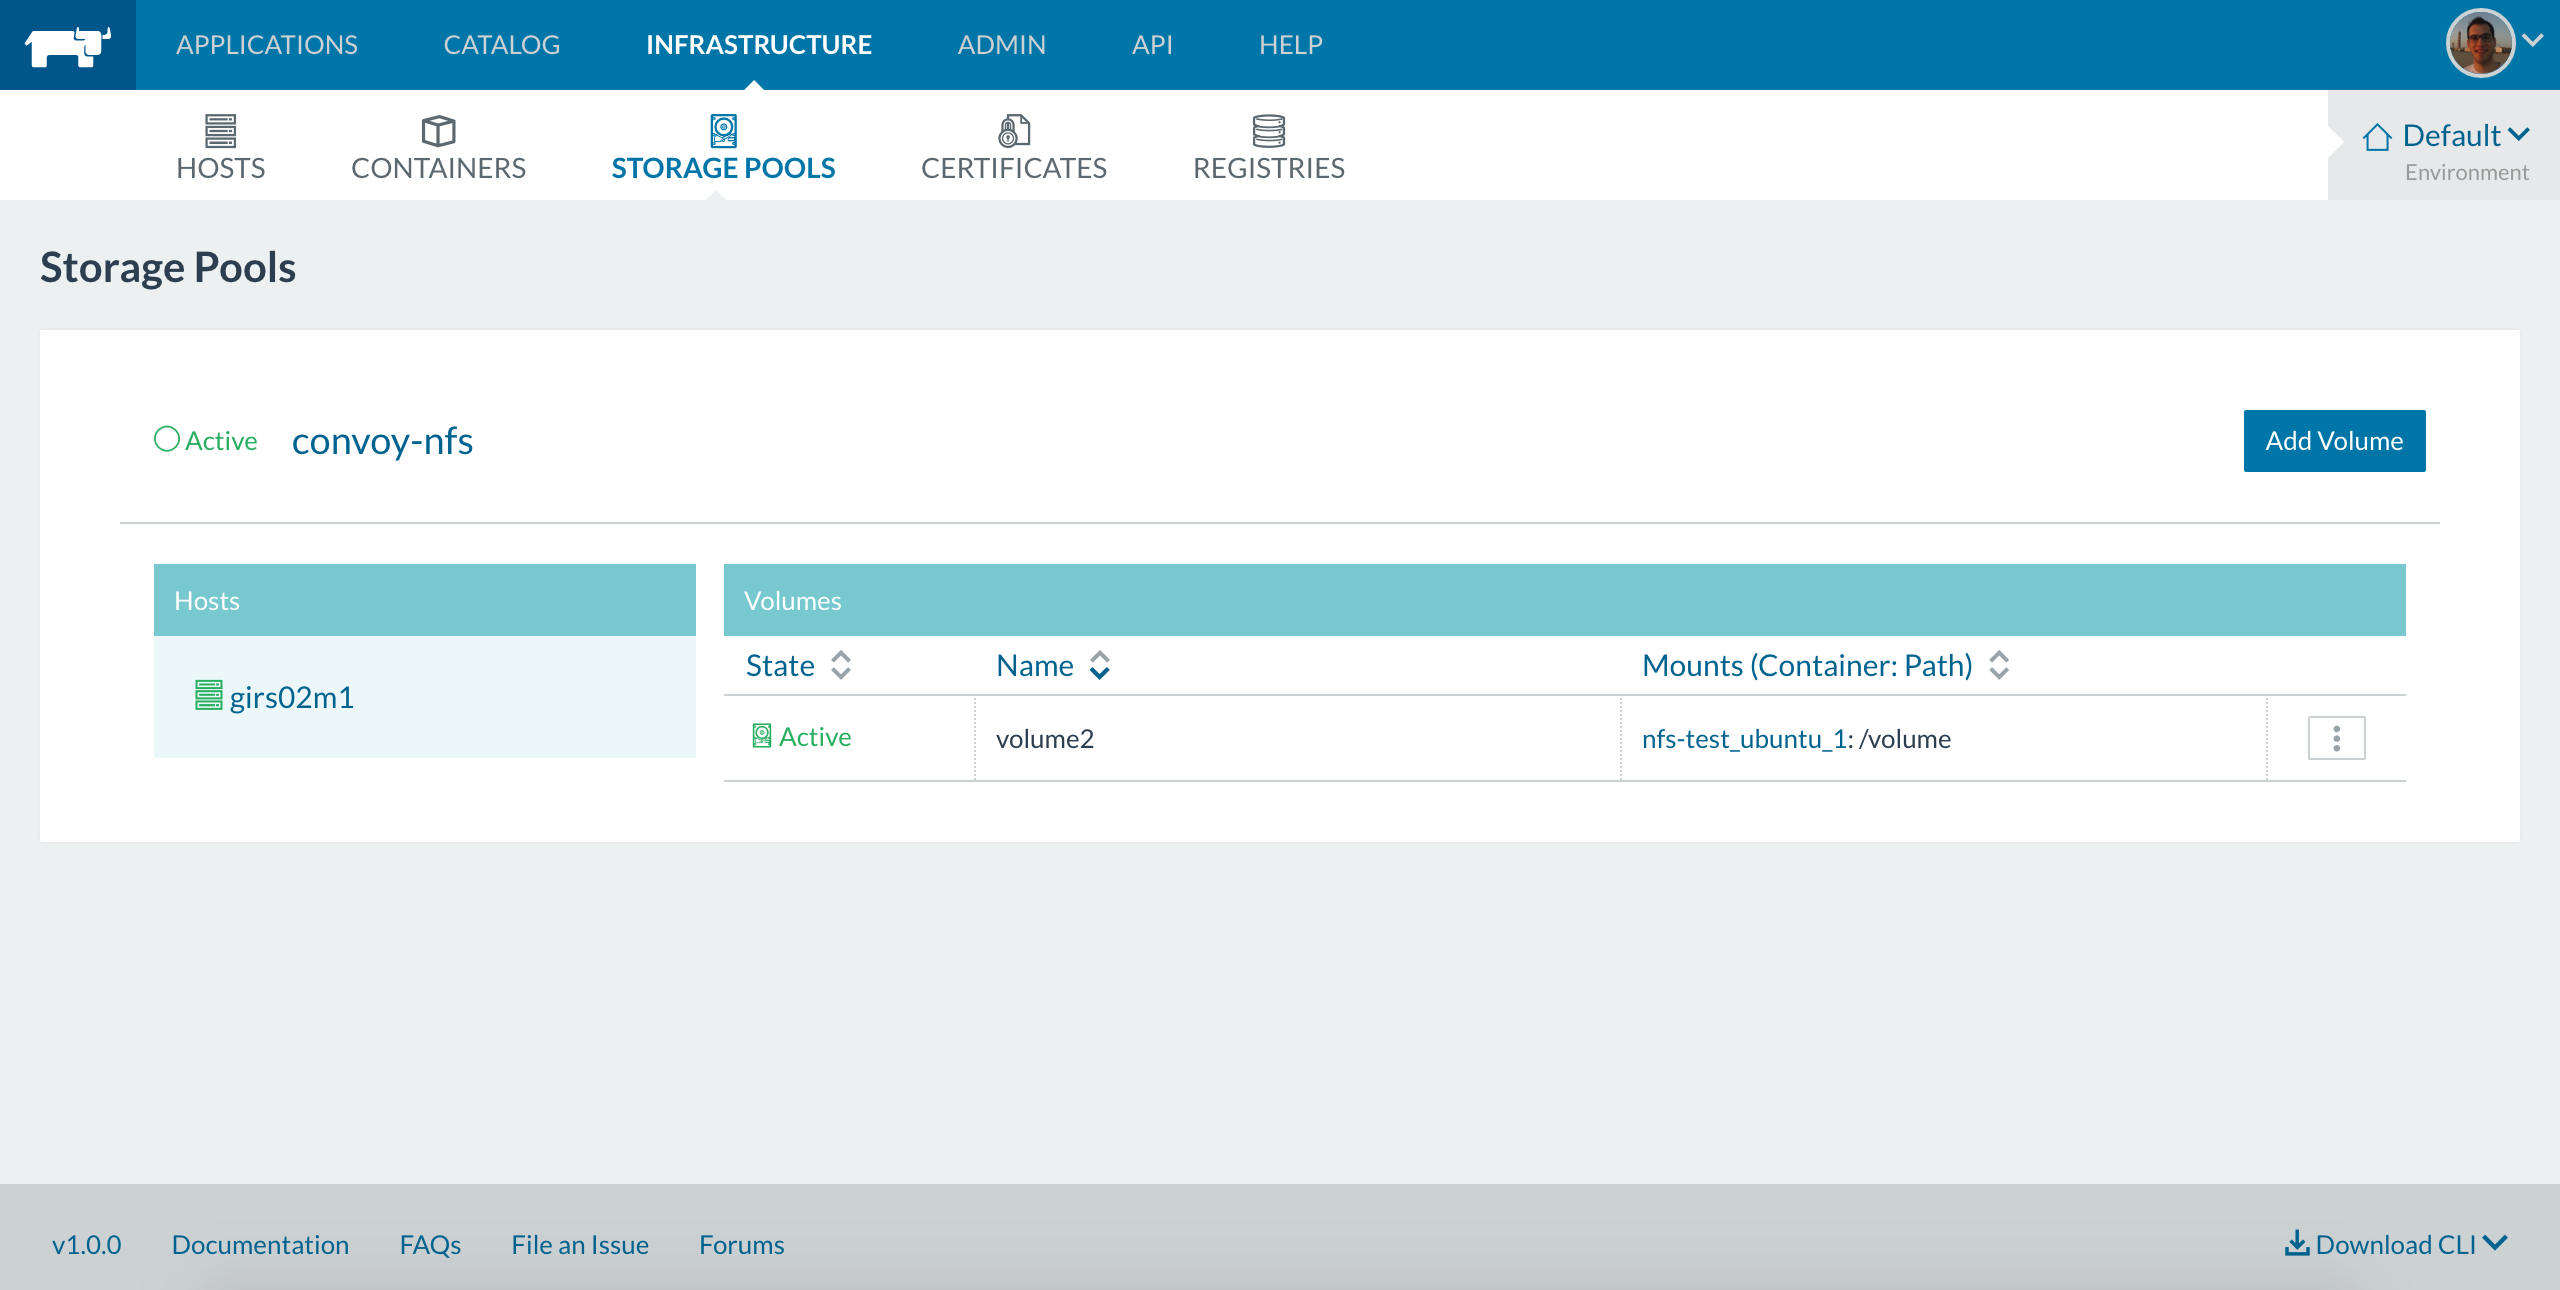
\includegraphics[width=65mm,scale=1]{imagens/storage_pools.png}
  \captionof{figure}{Storage pools}
  \label{fig:storage_pools}
\end{minipage}
\end{figure}


\begin{figure}[!htb]
\center
 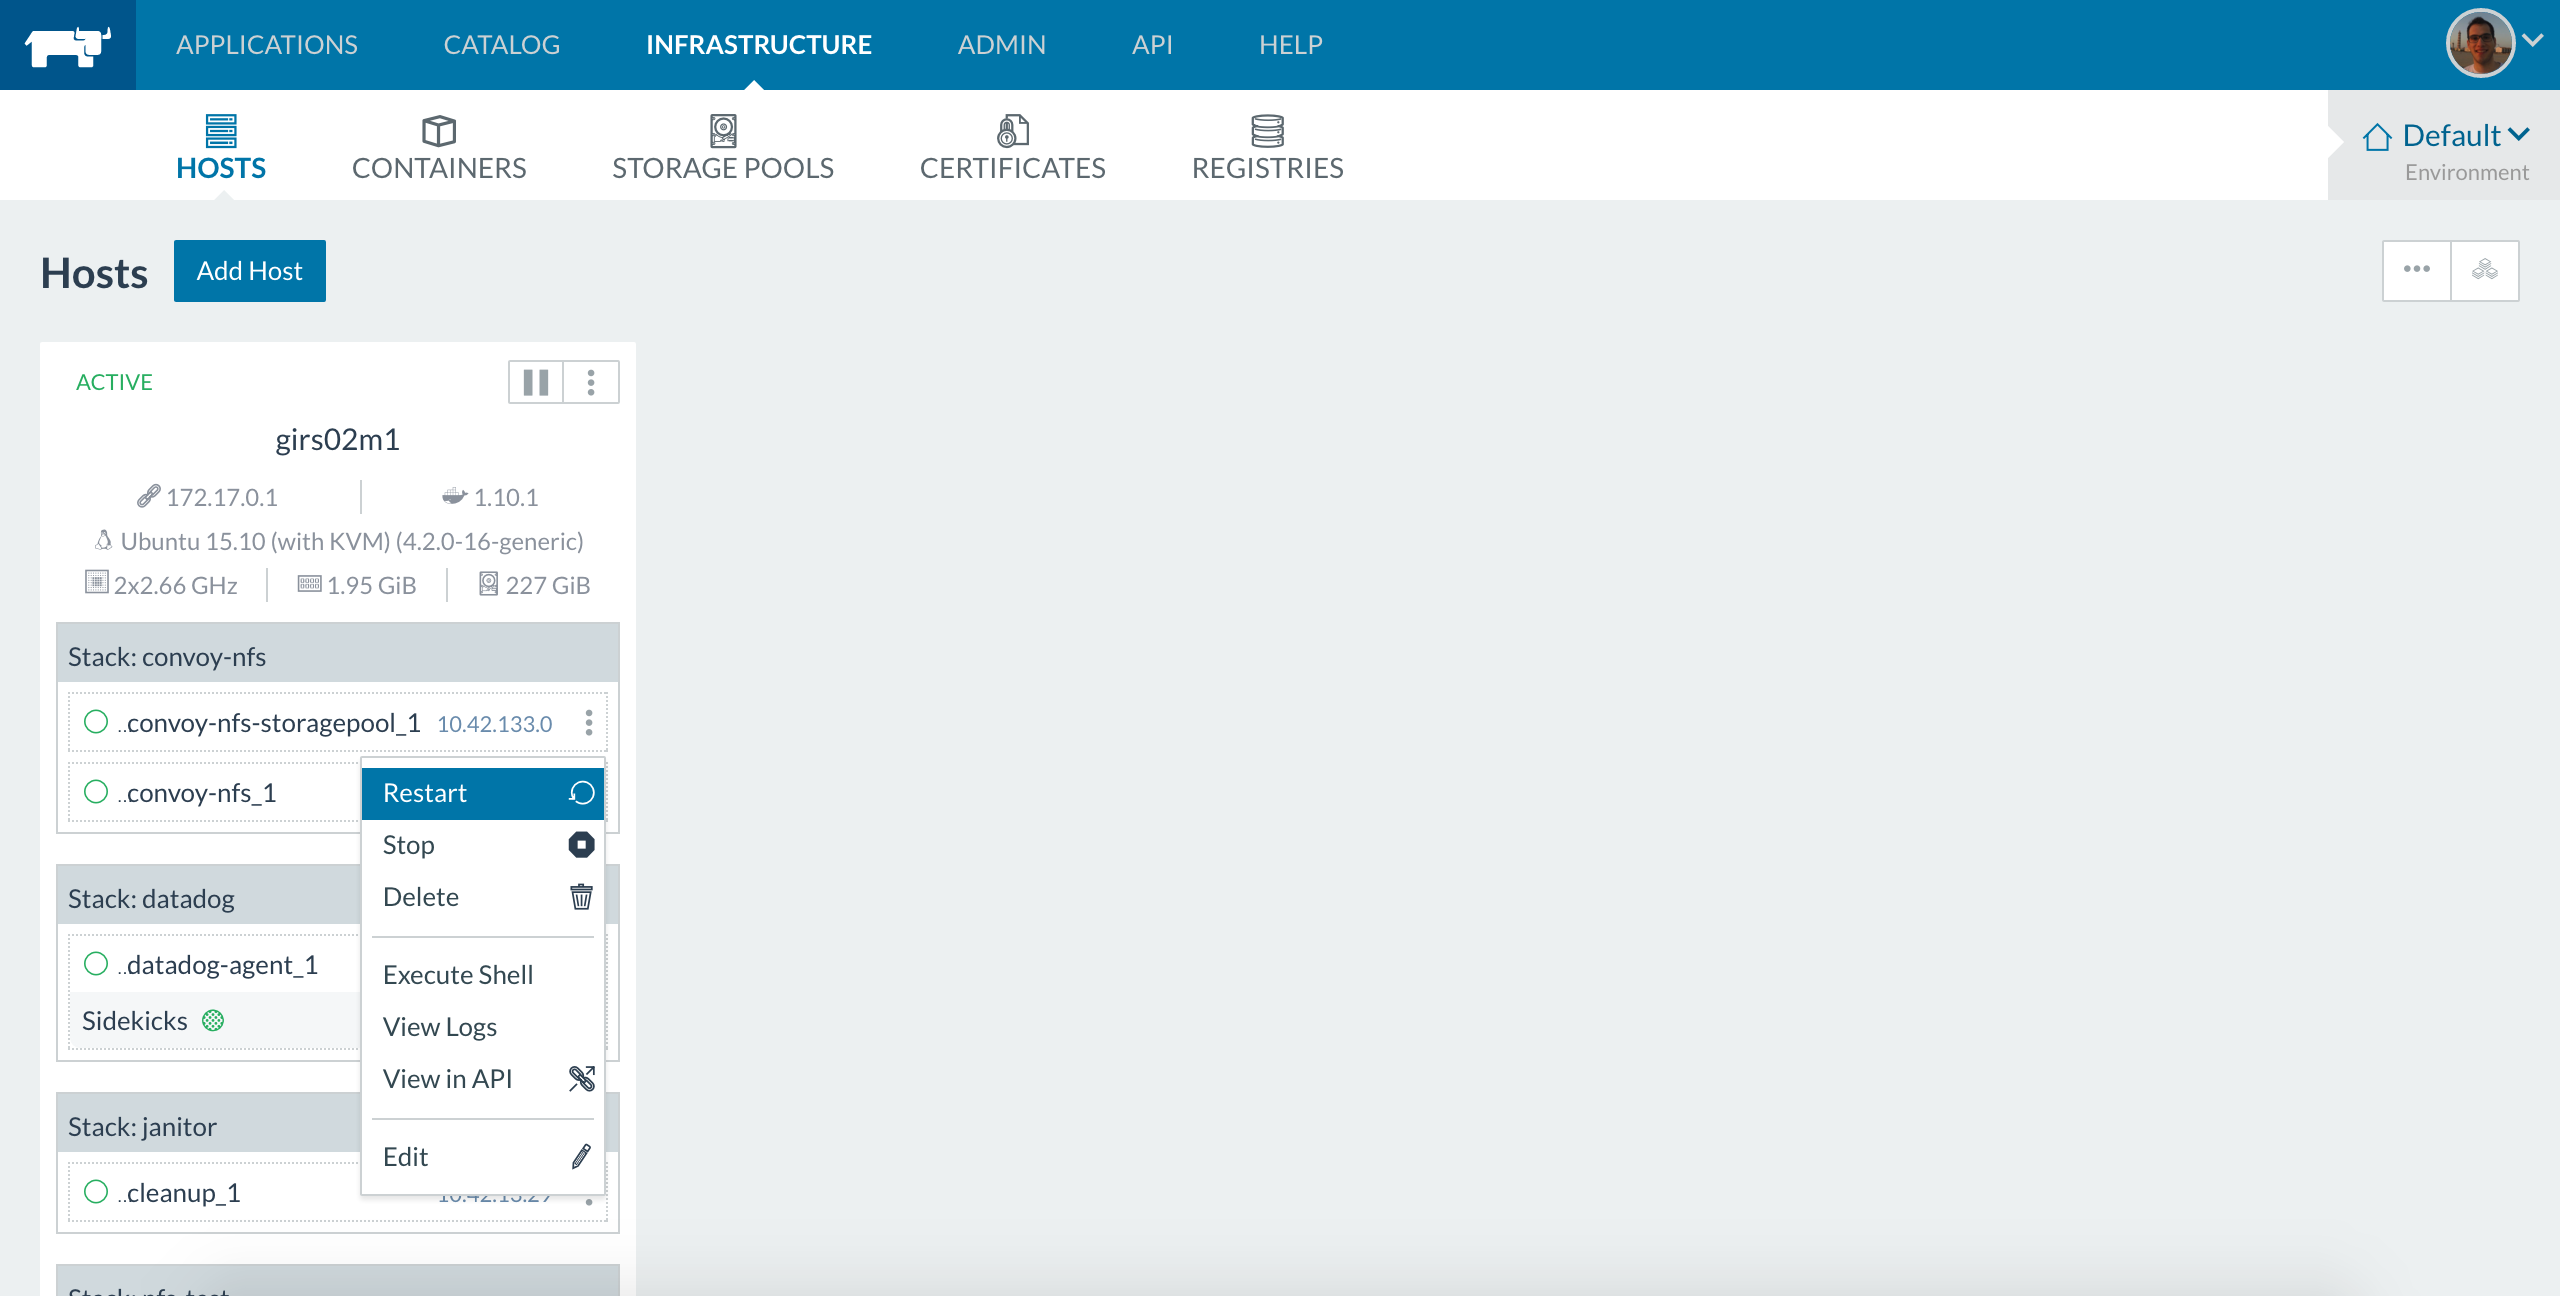
\includegraphics[width=150mm,scale=1]{imagens/hosts_menu.png}
 \caption{Hosts}
 \label{fig:hosts_menu}
\end{figure}


\section{Armazenamento}

\subsection{RAID}

\subsubsection{Criação de um RAID}

\subsubsection{Configuração}

\begin{figure}[!htb]
\center
 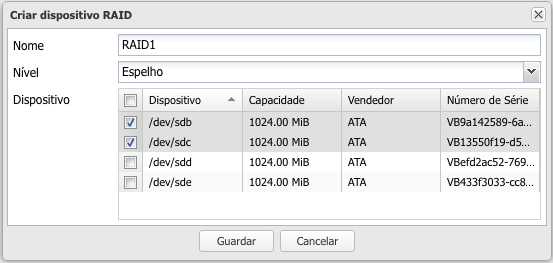
\includegraphics[width=150mm,scale=1]{imagens/RAID1Create.png}
 \caption{RAID 1}
 \label{fig:exemploraid}
\end{figure}

Para se avaliar os diferentes níveis de RAID usou-se o OpenMediaVault que é um sistema operativo para gestão de um NAS baseado em Debian (Linux).

Para instalação do ambiente foi criado uma máquina virtual usando a Virtual Box com 4 discos com 1024MB.

Depois foram criados diferentes níveis de RAID, sendo estes o nível 0, 1, 5, 6 e 10. Observou-se para os diferentes níveis de RAID, qual é o espaço disponível e removendo os discos, qual é o número de falhas que podem existir para que os dados não sejam perdidos. 

\begin{table}[!htb]
\centering
\caption{Avaliação dos diferentes níveis de RAID}
\label{my-label}
\begin{tabular}{|c|c|c|c|}
\hline
\multicolumn{1}{|l|}{\textbf{RAID}} & \multicolumn{1}{l|}{\textbf{Número de discos}} & \multicolumn{1}{l|}{\textbf{Espaço disponível}} & \multicolumn{1}{l|}{\textbf{Número de falhas permitidas}} \\ \hline
0                                   & 2                                              & 2 GB                                            & 0                                                        \\ \hline
1                                   & 2                                              & 1023.44 MB                                      & 1 (N-1)                                                  \\ \hline
10                                  & 4                                              & 2 GB                                            & 2 (N/2)                                                  \\ \hline
5                                   & 3                                              & 2 GB                                            & 1                                                        \\ \hline
6                                   & 4                                              & 2 GB                                            & 1                                                        \\ \hline
\end{tabular}
\end{table}

\subsection{NAS/SAN}

\subsubsection{Configuração do NAS}

Na segunda parte do trabalho foi pedido que fosse realizado uma NAS/SAN, para isso começou-se por criar um RAID 0 e criou-se um volume com o RAID 0 criado com o nome "md1" com o sistema de ficheiros "ext3". 

\begin{figure}[!htb]
\center
 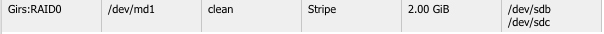
\includegraphics[width=150mm,scale=1]{imagens/RAID0.png}
 \caption{RAID 0}
 \label{fig:raid0}
\end{figure}

\begin{figure}[!htb]
\center
 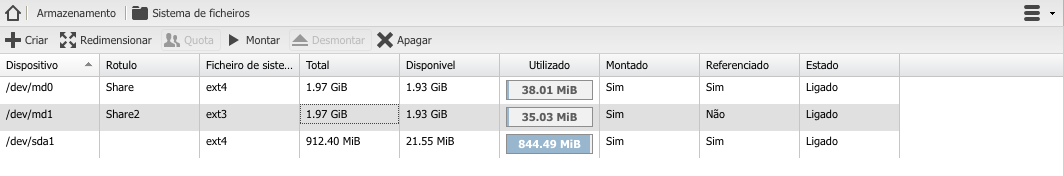
\includegraphics[width=150mm,scale=1]{imagens/FileSystem.png}
 \caption{Volume "md1"}
 \label{fig:exemploraid}
\end{figure}

Usando o Samba fez-se partilha do novo Volume criado como mostra a figura \ref{fig:SharedFolders}.

\begin{figure}[!htb]
\center
 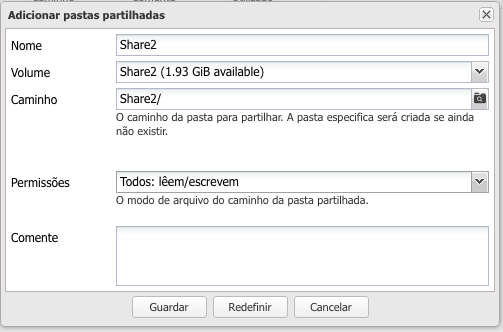
\includegraphics[width=100mm,scale=1]{imagens/AddShare2.png}
 \caption{Adicionar o Volume para partilha}
 \label{fig:SharedFolders}
\end{figure}

Depois montou-se a pasta partilhada como sendo um NAS num OS X como demonstra a figura \ref{fig:MacSharedFolders}.

\begin{figure}[!htb]
\center
 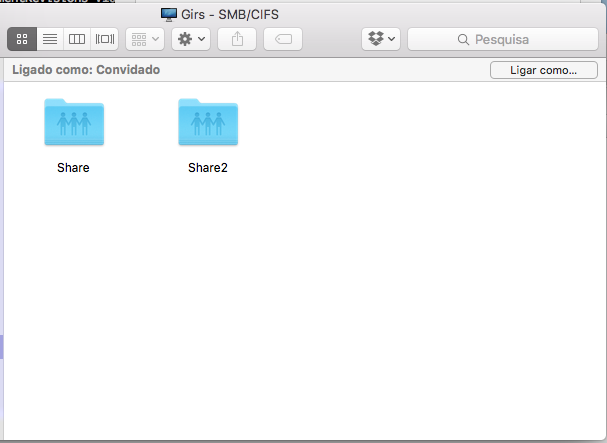
\includegraphics[width=80mm,scale=1]{imagens/MacSharedFolders.png}
 \caption{Pastas partilhadas}
 \label{fig:MacSharedFolders}
\end{figure}

\subsubsection{Teste do NAS}

Para testar se realmente estaria ou não a funcionar o NAS criado, criou-se um ficheiro na máquina virtual como demonstra a figura \ref{fig:CreateTestVM}.

\begin{figure}[!htb]
\center
 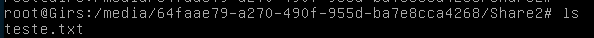
\includegraphics[width=80mm,scale=1]{imagens/CreateTestVM.png}
 \caption{Adicionar o Volume para partilha}
 \label{fig:CreateTestVM}
\end{figure}

Após isso, verificou-se se no OS X o ficheiro também já existia, e de facto, existia, como demonstra a figura \ref{fig:testMac.png}.

\begin{figure}[!htb]
\center
 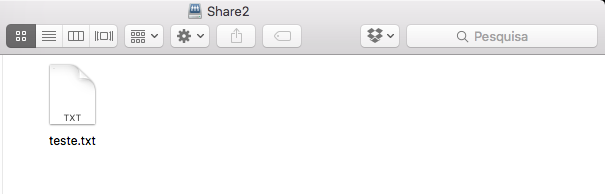
\includegraphics[width=80mm,scale=1]{imagens/testMac.png}
 \caption{Ficheiro existente no OS X}
 \label{fig:testMac}
\end{figure}

\subsubsection{Benchmark do NAS Volume}

Usando o "bonnie++" efetuaram-se 10 medições e calculou-se a média para obter resultados finais para a experiência, como mostram as tabelas \ref{table:bonnie++1}, \ref{table:bonnie++2} e \ref{table:bonnie++3}.

% Please add the following required packages to your document preamble:
% \usepackage[table,xcdraw]{xcolor}
% If you use beamer only pass "xcolor=table" option, i.e. \documentclass[xcolor=table]{beamer}
\begin{table}[!htb]
\centering
\caption{Resultados do benchmark usando bonnie++ (Parte 1)}
\label{table:bonnie++1}
\resizebox{\textwidth}{!}{\begin{tabular}{l|c|c|c|c|c|c|}
\cline{2-7}
                                                            & \cellcolor[HTML]{FFCC67}\textbf{Bonnie++ Version} & \cellcolor[HTML]{FFCC67}\textbf{Concurrency Level} & \cellcolor[HTML]{FFCC67}\textbf{Random Number Seed} & \cellcolor[HTML]{FFCC67}\textbf{File Size} & \cellcolor[HTML]{FFCC67}\textbf{Block Writes (K/s)} & \cellcolor[HTML]{FFCC67}\textbf{(\% cpu)} \\ \cline{2-7} 
                                                            & 1.97                                              & 1                                                  & 1459450816                                          & 8G                                         & 88149                                               & 10                                        \\ \cline{2-7} 
                                                            & 1.97                                              & 1                                                  & 1459453831                                          & 8G                                         & 72789                                               & 6                                         \\ \cline{2-7} 
                                                            & 1.97                                              & 1                                                  & 1459452397                                          & 8G                                         & 73546                                               & 7                                         \\ \cline{2-7} 
                                                            & 1.97                                              & 1                                                  & 1459452673                                          & 8G                                         & 75701                                               &                                           \\ \cline{2-7} 
                                                            & 1.97                                              & 1                                                  & 1459447167                                          & 8G                                         & 88738                                               & 9                                         \\ \cline{2-7} 
                                                            & 1.97                                              & 1                                                  & 1459446918                                          & 8G                                         & 72541                                               & 7                                         \\ \cline{2-7} 
                                                            & 1.97                                              & 1                                                  & 1459445918                                          & 8G                                         & 78299                                               & 7                                         \\ \cline{2-7} 
                                                            & 1.97                                              & 1                                                  & 1459449549                                          & 8G                                         & 75141                                               & 7                                         \\ \cline{2-7} 
                                                            & 1.97                                              & 1                                                  & 1459449100                                          & 8G                                         & 75521                                               & 7                                         \\ \cline{2-7} 
                                                            & 1.97                                              & 1                                                  & 1459449032                                          & 8G                                         & 80327                                               & 8                                         \\ \hline
\rowcolor[HTML]{FFFC9E} 
\multicolumn{1}{|c|}{\cellcolor[HTML]{F8A102}\textbf{média}} & {\color[HTML]{333333} \textbf{1.97}}              & {\color[HTML]{333333} \textbf{1}}                  & {\color[HTML]{333333} \textbf{1459449740}}          & {\color[HTML]{333333} \textbf{8G}}         & {\color[HTML]{333333} \textbf{78075,2}}             & {\color[HTML]{333333} \textbf{7,5}}       \\ \hline
\end{tabular}}
\end{table}


% Please add the following required packages to your document preamble:
% \usepackage[table,xcdraw]{xcolor}
% If you use beamer only pass "xcolor=table" option, i.e. \documentclass[xcolor=table]{beamer}
\begin{table}[!htb]
\centering
\caption{Resultados do benchmark usando bonnie++ (Parte 2)}
\label{table:bonnie++2}
\resizebox{\textwidth}{!}{\begin{tabular}{l|c|c|c|c|c|c|}
\cline{2-7}
                                                            & \cellcolor[HTML]{FFCC67}\textbf{Reading/Rewriting Block (K/s)} & \cellcolor[HTML]{FFCC67}\textbf{(\% cpu)} & \cellcolor[HTML]{FFCC67}\textbf{Block Reads (K/s)} & \cellcolor[HTML]{FFCC67}\textbf{(\% cpu)} & \cellcolor[HTML]{FFCC67}\textbf{Seek (s/s)} & \cellcolor[HTML]{FFCC67}\textbf{(\% cpu)} \\ \cline{2-7} 
                                                            & 21758                                                          & 6                                         & 47470                                              & 5                                         & 1000                                        & 31                                        \\ \cline{2-7} 
                                                            & 32983                                                          & 5                                         & 77413                                              & 8                                         & 940,2                                       & 27                                        \\ \cline{2-7} 
                                                            & 38005                                                          & 6                                         & 77339                                              & 7                                         & 1103                                        & 35                                        \\ \cline{2-7} 
                                                            & 30252                                                          & 6                                         & 71017                                              & 7                                         & 1060                                        & 35                                        \\ \cline{2-7} 
                                                            & 32433                                                          & 10                                        & 73999                                              & 7                                         & 1055                                        & 33                                        \\ \cline{2-7} 
                                                            & 36601                                                          & 6                                         & 74004                                              & 7                                         & 1004                                        & 32                                        \\ \cline{2-7} 
                                                            & 32597                                                          & 6                                         & 66784                                              & 7                                         & 1093                                        & 34                                        \\ \cline{2-7} 
                                                            & 31529                                                          & 6                                         & 71241                                              & 7                                         & 907,1                                       & 29                                        \\ \cline{2-7} 
                                                            & 33710                                                          & 6                                         & 74052                                              & 7                                         & 994,8                                       & 31                                        \\ \cline{2-7} 
                                                            & 32089                                                          & 5                                         & 73297                                              & 7                                         & 973,5                                       & 31                                        \\ \hline
\rowcolor[HTML]{FFFC9E} 
\multicolumn{1}{|c|}{\cellcolor[HTML]{F8A102}\textbf{média}} & {\color[HTML]{333333} \textbf{32195,7}}                        & {\color[HTML]{333333} \textbf{6,2}}       & {\color[HTML]{333333} \textbf{70661,6}}            & {\color[HTML]{333333} \textbf{6,9}}       & {\color[HTML]{333333} \textbf{1013,06}}     & {\color[HTML]{333333} \textbf{31,8}}      \\ \hline
\end{tabular}}
\end{table}

% Please add the following required packages to your document preamble:
% \usepackage[table,xcdraw]{xcolor}
% If you use beamer only pass "xcolor=table" option, i.e. \documentclass[xcolor=table]{beamer}
\begin{table}[!htb]
\centering
\caption{Resultados do benchmark usando bonnie++ (Parte 3)}
\label{table:bonnie++3}
\resizebox{\textwidth}{!}{\begin{tabular}{l|c|c|c|l|}
\cline{2-5}
                                                            & \cellcolor[HTML]{FFCC67}\textbf{Block Write Latency (ms)} & \cellcolor[HTML]{FFCC67}\textbf{Rewrite Latency (ms)} & \cellcolor[HTML]{FFCC67}\textbf{Block Read Latency (ms)} & \cellcolor[HTML]{FFCC67}\textbf{Seek Latency (ms)} \\ \cline{2-5} 
                                                            & 4009                                                      & 11369                                                 & 11902                                                    & 175                                                \\ \cline{2-5} 
                                                            & 27544                                                     & 11565                                                 & 10906                                                    & 3186                                               \\ \cline{2-5} 
                                                            & 5024                                                      & 25956                                                 & 11947                                                    & 1697                                               \\ \cline{2-5} 
                                                            & 5512                                                      & 10859                                                 & 9862                                                     & 168                                                \\ \cline{2-5} 
                                                            & 4185                                                      & 21276                                                 & 10784                                                    & 2173                                               \\ \cline{2-5} 
                                                            & 4909                                                      & 12442                                                 & 11381                                                    & 2292                                               \\ \cline{2-5} 
                                                            & 5541                                                      & 10699                                                 & 11237                                                    & 178                                                \\ \cline{2-5} 
                                                            & 6399                                                      & 11024                                                 & 11982                                                    & 169                                                \\ \cline{2-5} 
                                                            & 5440                                                      & 11958                                                 & 13269                                                    & 171                                                \\ \cline{2-5} 
                                                            & 4428                                                      & 34282                                                 & 11390                                                    & 182                                                \\ \hline
\rowcolor[HTML]{FFFC9E} 
\multicolumn{1}{|c|}{\cellcolor[HTML]{F8A102}\textbf{média}} & {\color[HTML]{333333} \textbf{7299,1}}                    & {\color[HTML]{333333} \textbf{16143}}                 & {\color[HTML]{333333} \textbf{11466}}                    & {\color[HTML]{333333} \textbf{1039,1}}             \\ \hline
\end{tabular}}
\end{table}

\newpage

No final concluiu-se que para o mesmo nível de concorrência e para a escrita e leitura de um ficheiro com o tamanho de 8GB que: 

% Please add the following required packages to your document preamble:
% \usepackage[table,xcdraw]{xcolor}
% If you use beamer only pass "xcolor=table" option, i.e. \documentclass[xcolor=table]{beamer}
\begin{table}[!htb]
\centering
\caption{Resultados finais da benchmark bonnie++}
\label{table:resultados_bonnie}
\resizebox{\textwidth}{!}{\begin{tabular}{|
>{\columncolor[HTML]{FFCE93}}l |c|
>{\columncolor[HTML]{FFCE93}}l |c|}
\hline
\textbf{Block Writes (K/s)}            & 78075,2 & \textbf{Seek (s/s)}               & 1013,06 \\ \hline
\textbf{(\% cpu)}                      & 7,5     & \textbf{(\% cpu)}                 & 31,8    \\ \hline
\textbf{Reading/Rewriting Block (K/s)} & 32195,7 & \textbf{Block Write Latency (ms)} & 7299,1  \\ \hline
\textbf{(\% cpu)}                      & 6,2     & \textbf{Rewrite Latency (ms)}     & 16143   \\ \hline
\textbf{Block Reads (K/s)}             & 70661,6 & \textbf{Block Read Latency (ms)}  & 11466   \\ \hline
\textbf{(\% cpu)}                      & 6,9     & \textbf{Seek Latency (ms)}        & 1039,1  \\ \hline
\end{tabular}}
\end{table}

\newpage

Esta tabela permitiu que se percebesse melhor os sistemas de RAID existentes. Entre eles existe, por exemplo o RAID 0, que é o ideal quando se procura uma melhor performance. Existe ainda para uma maior capacidade de armazenamento o JBOD e para melhor redundância, com melhor aproveitamento de discos, podendo falhar até dois, tem-se o RAID 6.

Foi ainda possível, através da benchmark Bonnie++, ter conhecimento acerca dos tempos de escrita e leitura numa pasta partilhada na rede pela NAS criada no trabalho.


\subsection{Rancher Storage Pool}

Usando uma máquina do laboratório, instalou-se uma imagem de Ubuntu Server e colocou-se NFS.

\begin{figure}[!htb]
\center
 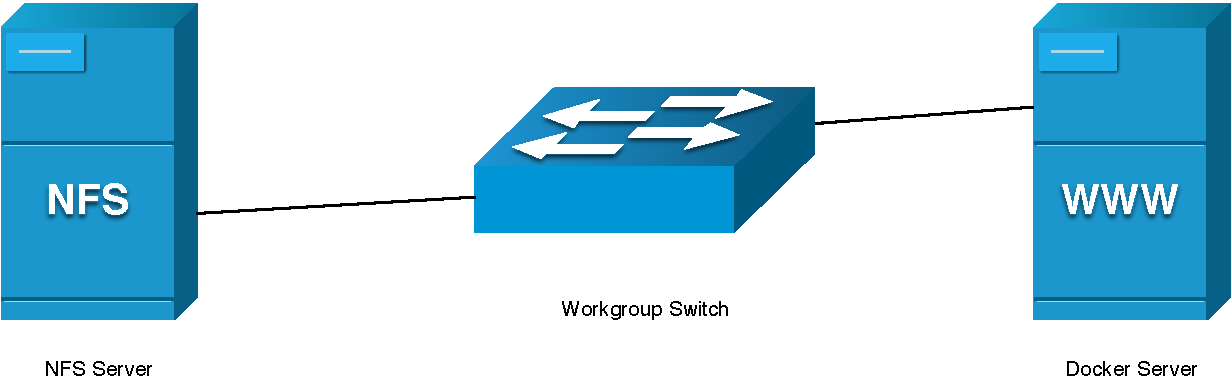
\includegraphics[width=80mm,scale=1]{imagens/servers.pdf}
 \caption{Arquitetura de servidores}
 \label{fig:servers}
\end{figure}

Usando o Convoy NFS\footnote{\label{url1} \url{https://github.com/rancher/convoy}} foi montado o NFS do servidor paralelo no Rancher. 

Depois de montado, o NFS, devem ser criados vários volumes que depois serão usados para os containers que serão instanciados. Esta solução permite que os ficheiros do container estejam num servidor à parte de storage, sendo mais fácil efetuar backups aos dados de todos os containers.

Os volumes criados só irão aparecer ativos quando forem usados num container.

\begin{figure}[!htb]
\centering
\begin{minipage}{.5\textwidth}
  \centering
  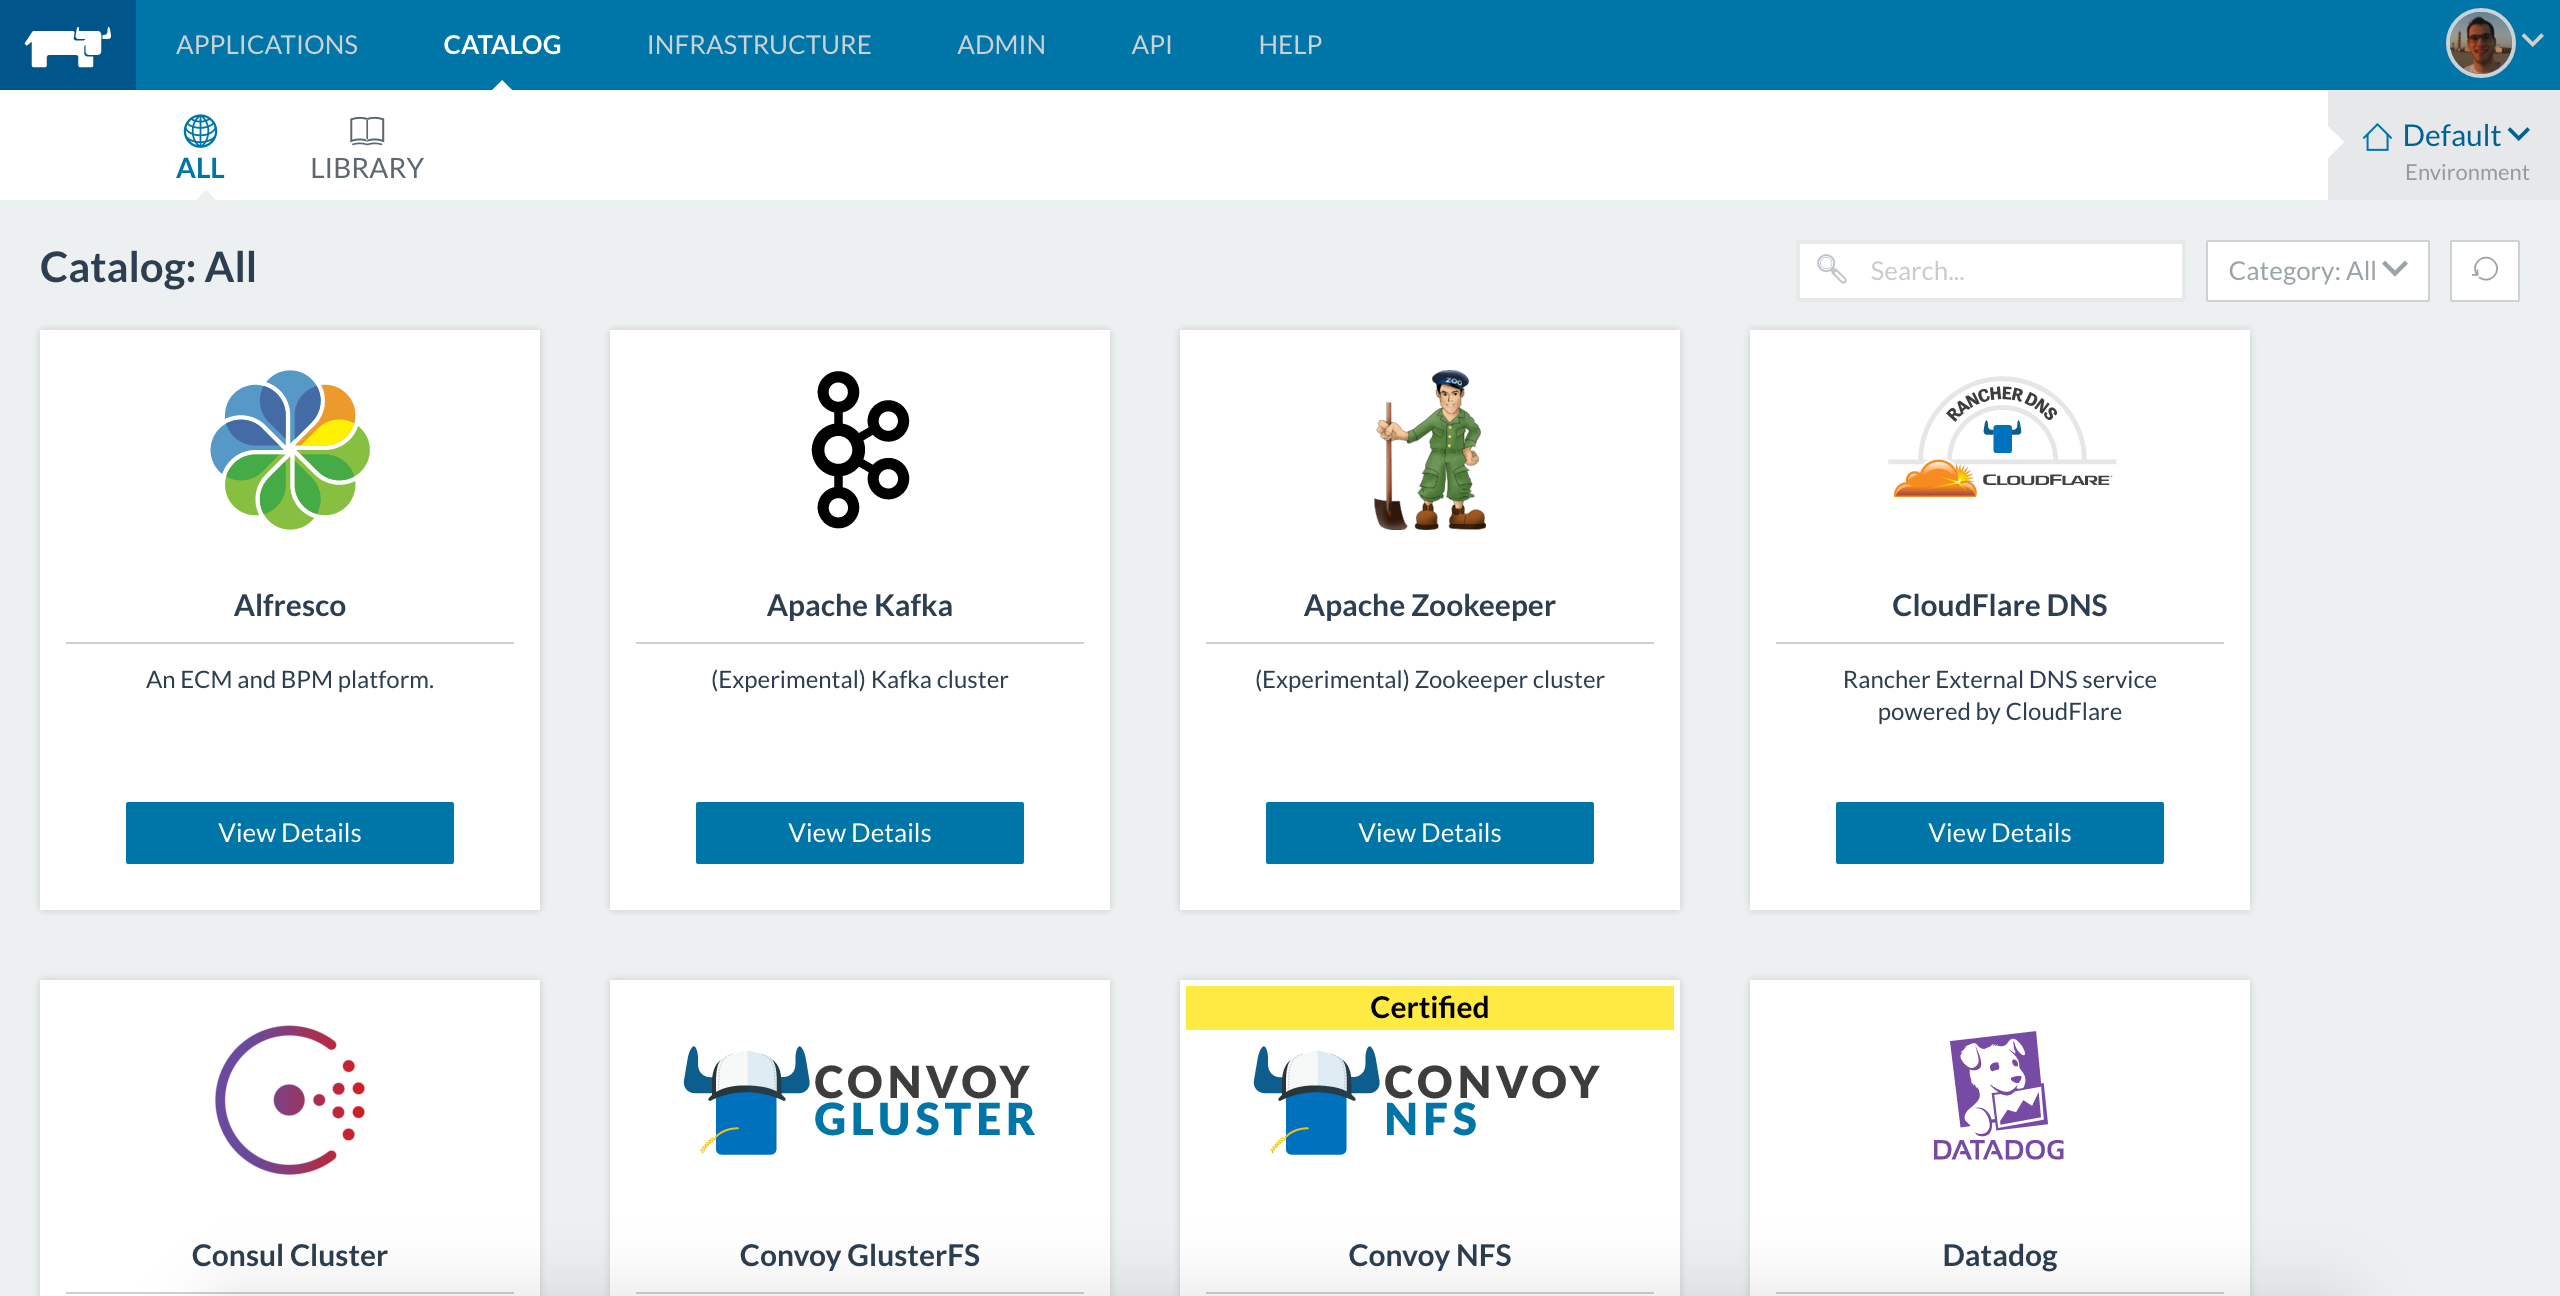
\includegraphics[width=65mm,scale=1]{imagens/catalog_all.png}
  \captionof{figure}{Convoy NFS Catalog}
  \label{fig:catalog_all}
\end{minipage}%
\begin{minipage}{.5\textwidth}
  \centering
  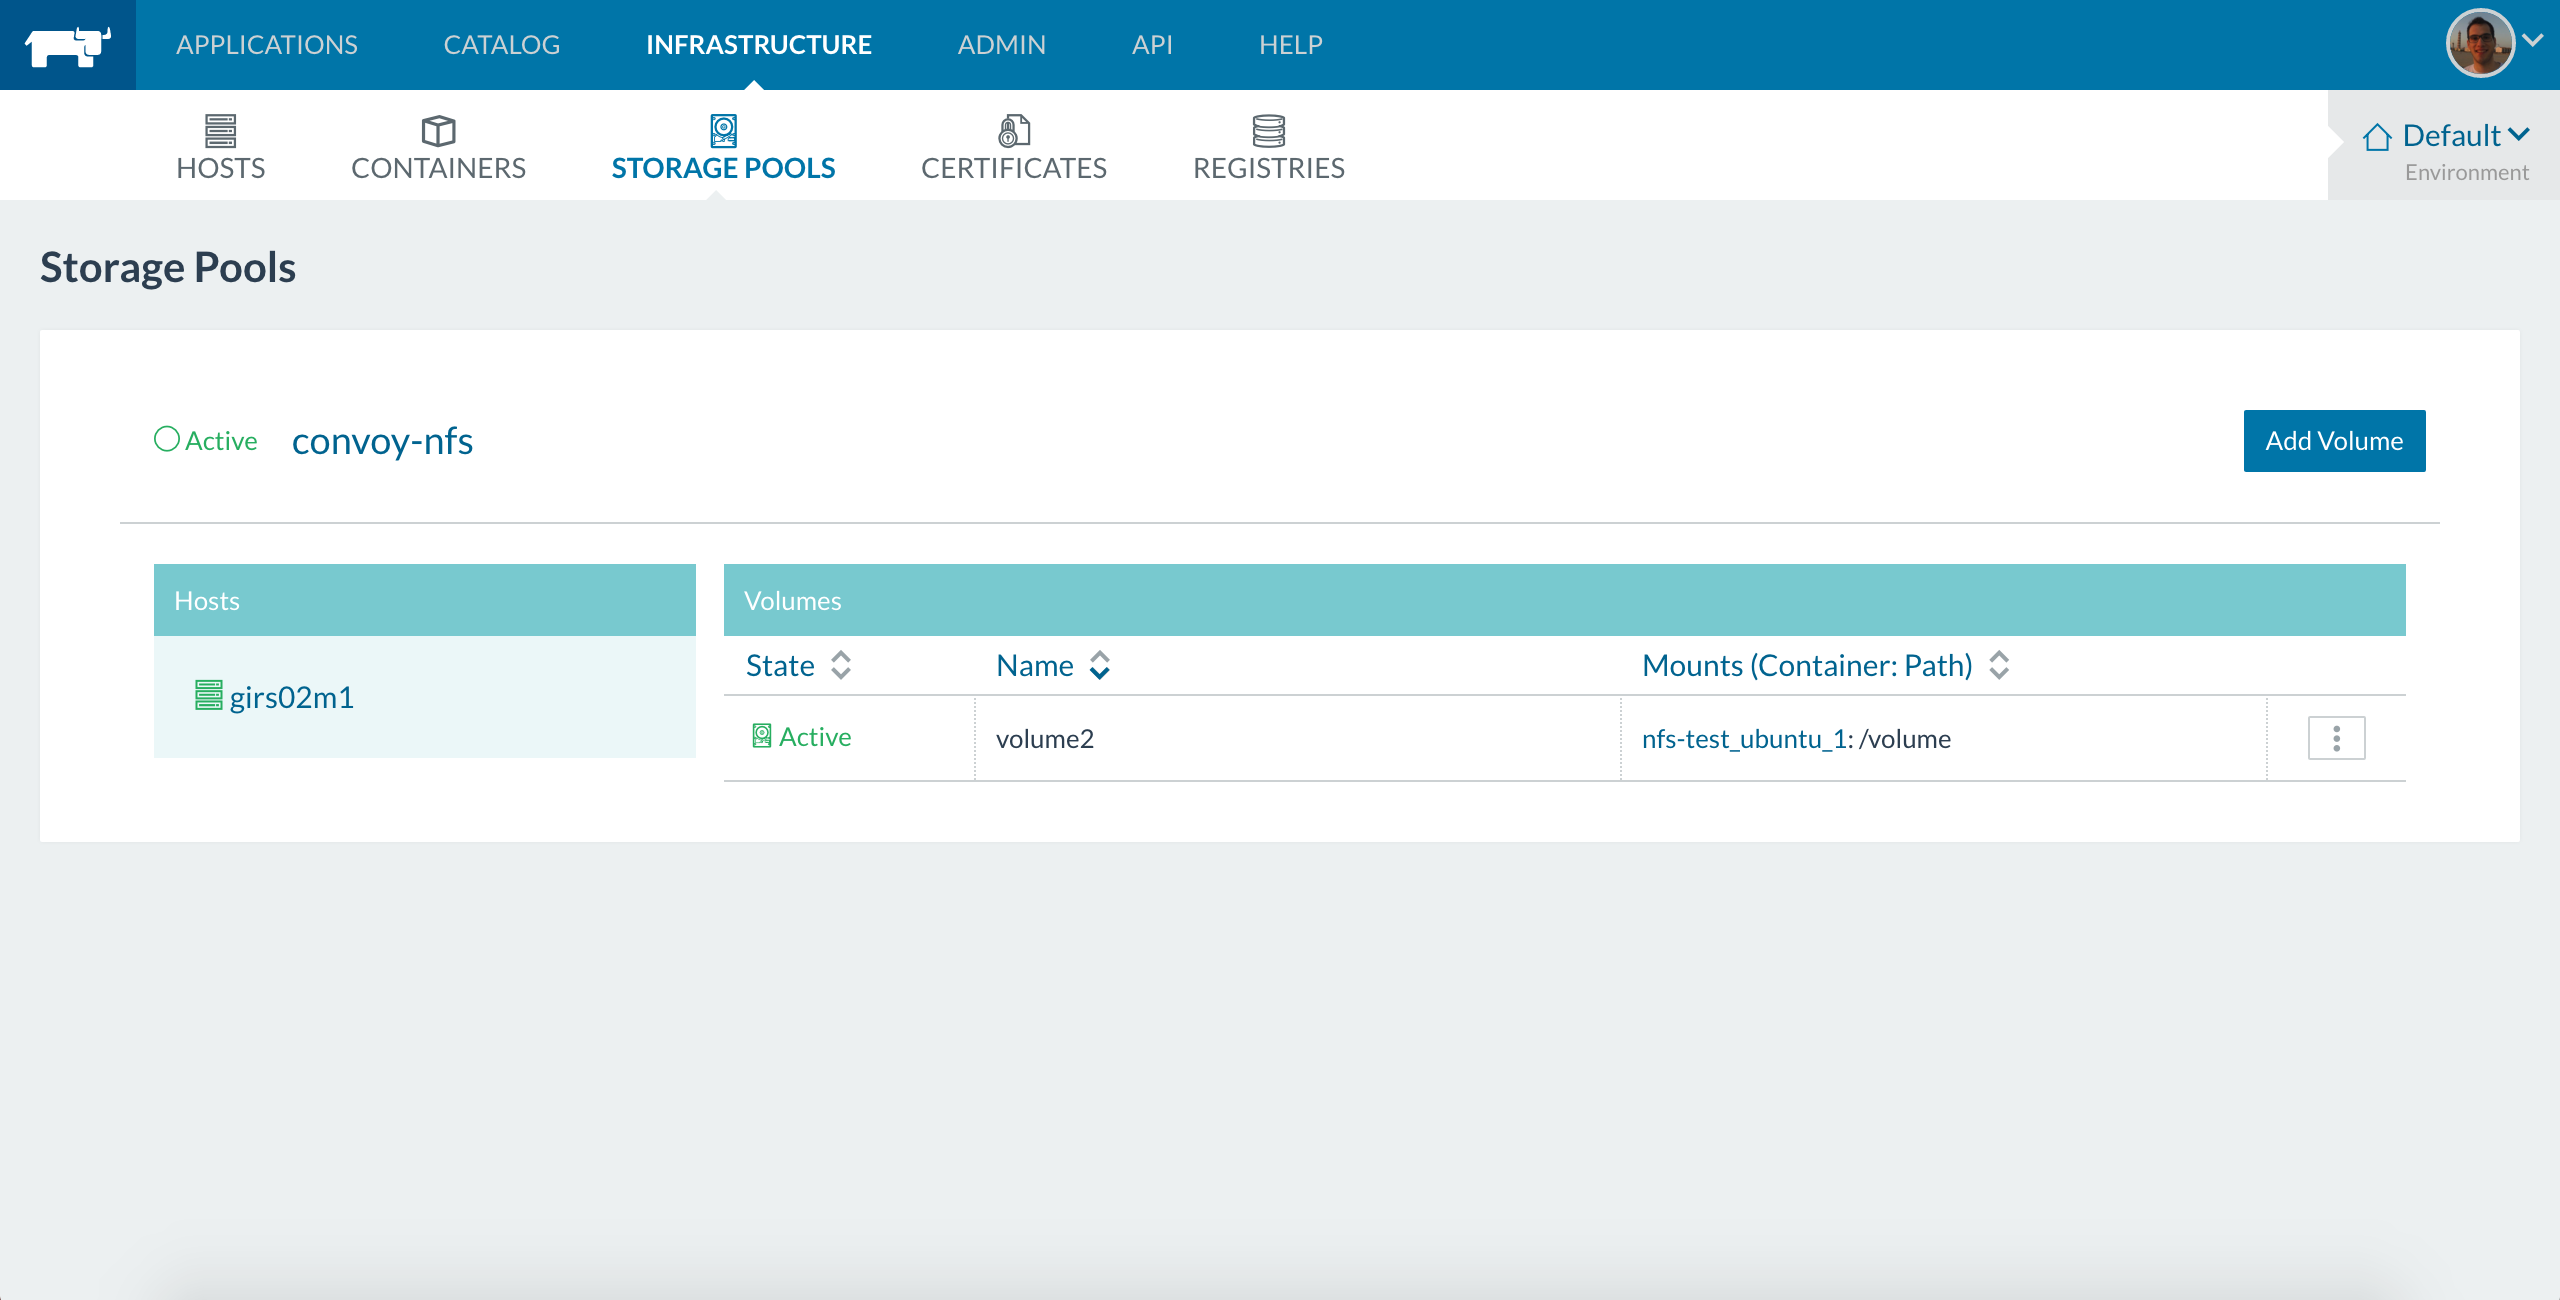
\includegraphics[width=65mm,scale=1]{imagens/storage_pools_volumes.png}
  \captionof{figure}{Volumes criados no Convoy NFS}
  \label{fig:storage_pools_volumes}
\end{minipage}
\end{figure}

\subsubsection{Volume NFS num Container}

Para testar a criação de um container com um Volume NFS, foi criado uma Stack "nfs-test" com um container com uma imagem "ubuntu:14.04.3" com um volume a fazer mount no diretório "/volume", apenas para efeito de teste.

Foi então criado um ficheiro "rafa" no diretório "/volume" com o conteúdo de "ola". 
\newpage

\begin{figure}[!htb]
\center
 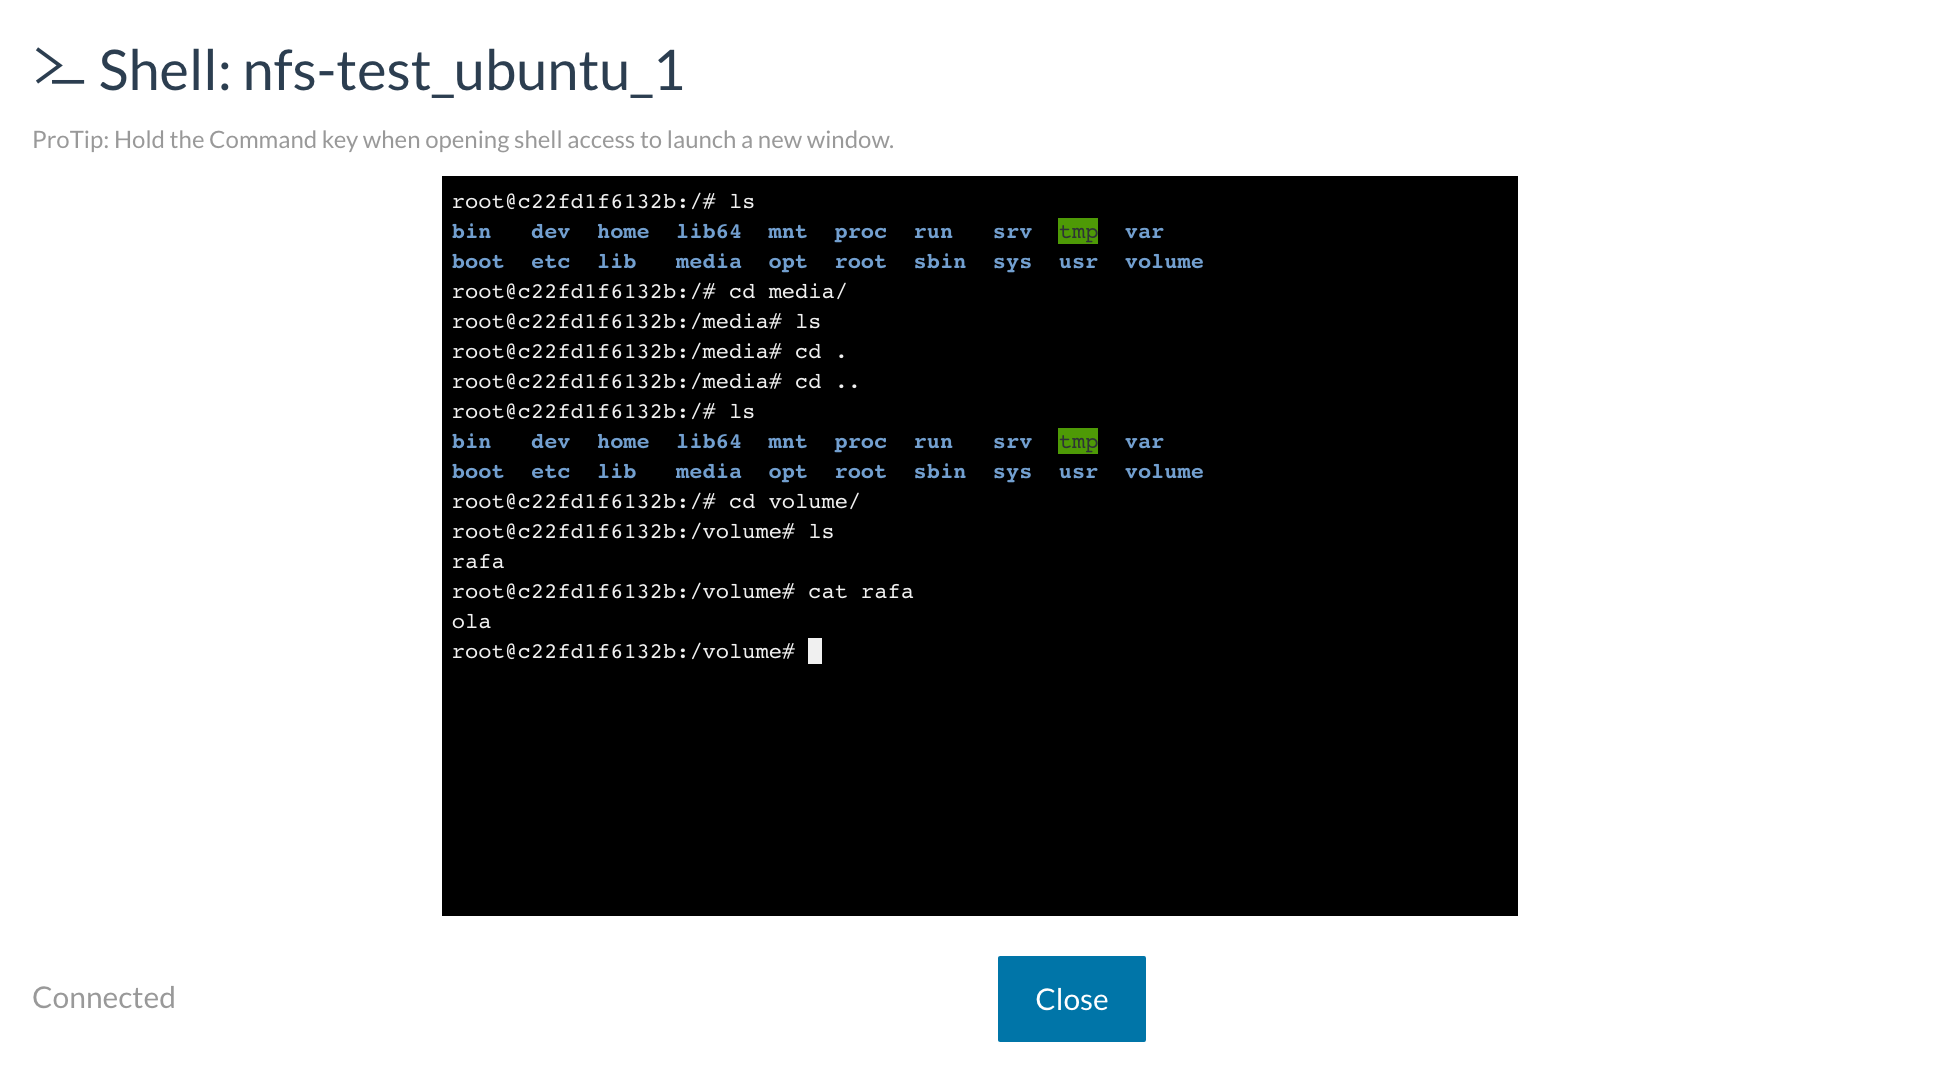
\includegraphics[width=150mm,scale=1]{imagens/nfs_container_show.png}
 \caption{Criação de um ficheiro no diretório "volume"}
 \label{fig:nfs_container_show}
\end{figure}

Depois, para testar, acedeu-se à máquina NFS e listou-se o diretório partilhado com a máquina Docker, e observou-se que o ficheiro também tinha sido ali criado.

\begin{figure}[!htb]
\center
 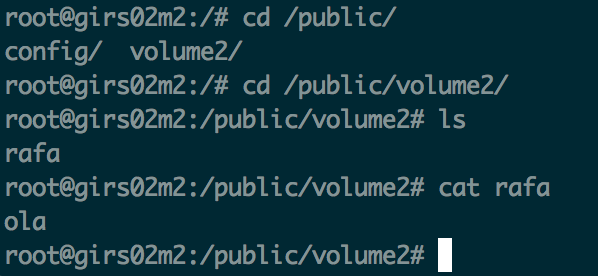
\includegraphics[width=100mm,scale=]{imagens/girsm2_show_nfs.png}
 \caption{Máquina NFS}
 \label{fig:girsm2_show_nfs}
\end{figure}



\section{Monitorização}

\subsection{Centreon}

Para a realização da parte de monitorização do projeto, foi utilizada a plataforma Centreon \footnote{\label{url2} \url{https://www.centreon.com/en/}}. Esta plataforma consiste numa ferramenta de supervisão e monitorização de uma rede, baseando-se no mecanismo de monitorização OpenSource, Nagios \footnote{\label{url3} \url{https://www.nagios.org/}}.

\begin{figure}[!htb]
\center
 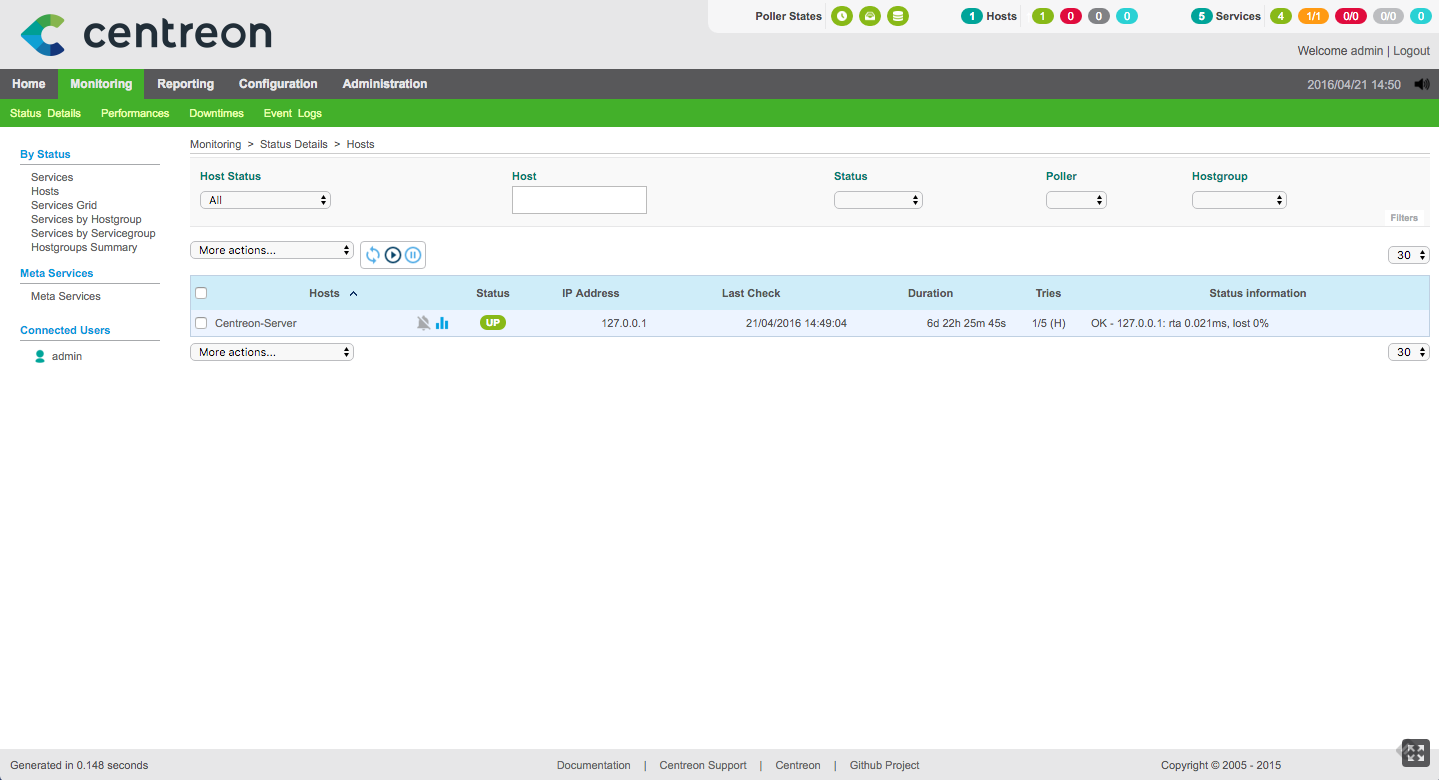
\includegraphics[width=150mm,scale=1]{imagens/CentreonPrincipal.png}
 \caption{Lista de Hosts, ambiente Centreon}
 \label{fig:centreonPrincipal}
\end{figure}

\newpage
Todos os testes de monitorização realizados, são serviços criados no host "Centreon-Server". Na imagem abaixo, é possível ver os testes criados:

\begin{figure}[!htb]
\center
 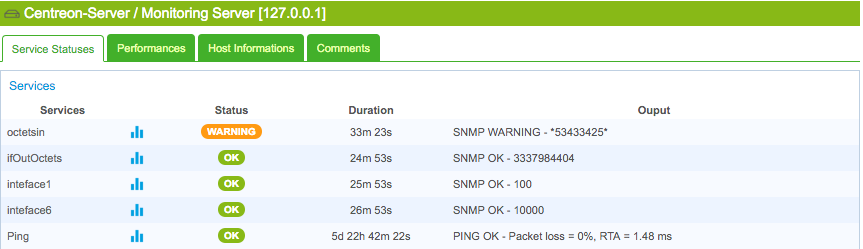
\includegraphics[width=150mm,scale=1]{imagens/ServicesList.png}
 \caption{Lista de Serviços do Host "Centreon-Server"}
 \label{fig:centreonPrincipal}
\end{figure}

Para cada serviço, foi criado um comando, que é o executado na máquina Centreon, que opera sobre o router, pois a máquina do grupo, que possui Docker, não disponibilizava as MIBS necessárias para a obtenção de dados interessantes, tendo por isto sido proposta pelo professor, a monitorização ao router.

Um exemplo da configuração de um comando é o seguinte:

\begin{figure}[!htb]
\center
 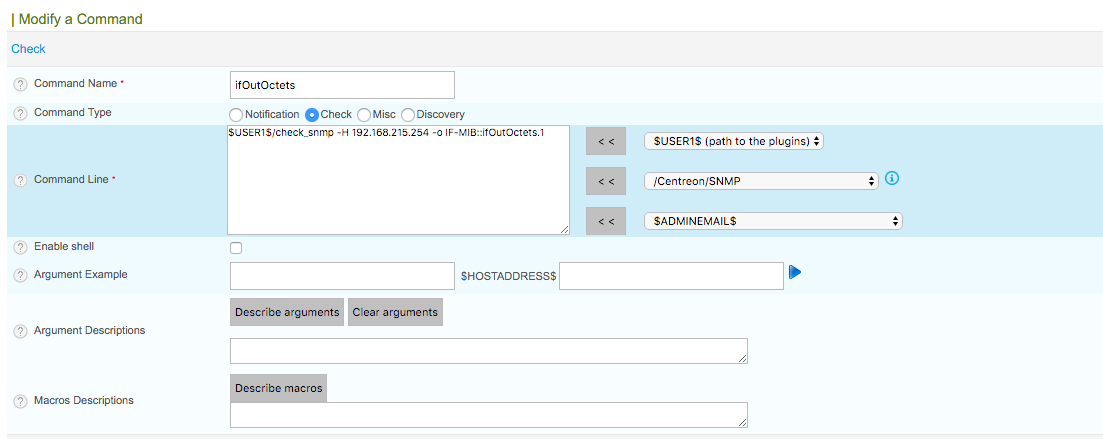
\includegraphics[width=150mm,scale=1]{imagens/ConfiguracaoComando.png}
 \caption{Painel de configuração de um comando}
 \label{fig:comando}
\end{figure}

Neste caso acima apresentado, o comando consiste num pedido de informação relativamente à quantidade de octetos que saem na interface 1.

Estes comandos criados, podem ser posteriormente utilizados por serviços criados para um host ou grupo de hosts. A configuração de um serviço consiste no seguinte:

\begin{figure}[!htb]
\center
 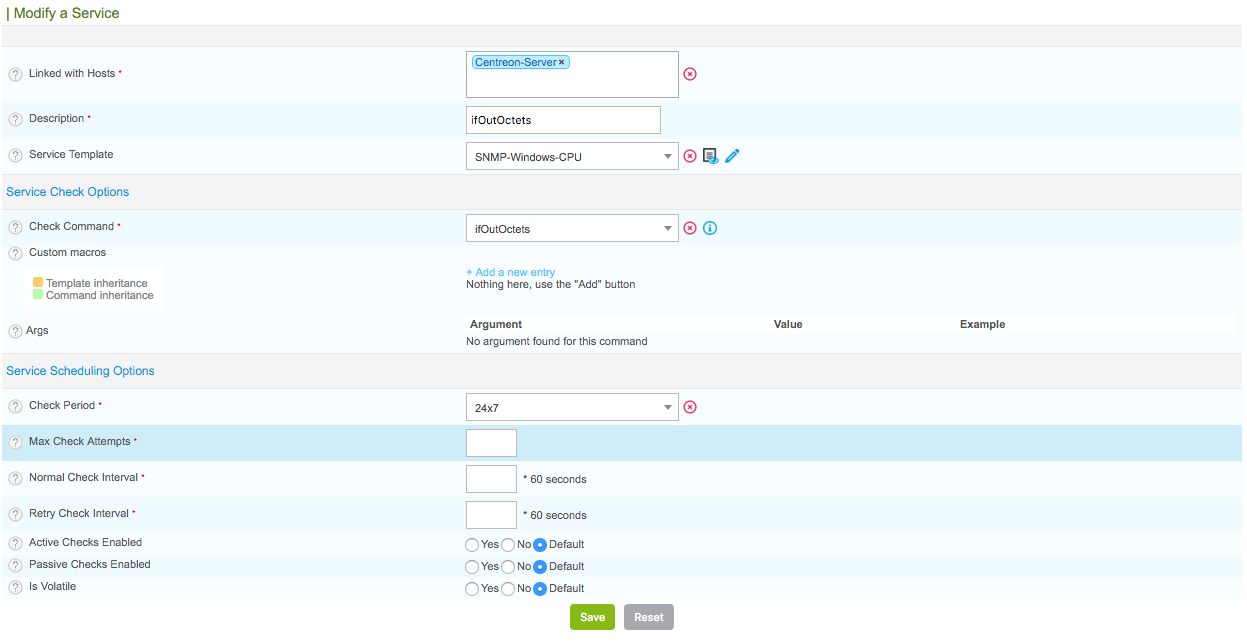
\includegraphics[width=150mm,scale=1]{imagens/ConfiguracaoService.png}
 \caption{Painel de configuração de um serviço}
 \label{fig:service}
\end{figure}

Para configurar o serviço que fornece a informação acerca dos octetos que saem da interface 1, seleciona-se o conjunto de hosts que possuirá o serviço a ser criado. Neste serviço, escolhe-se o comando criado previamente.

Depois de todos os serviços criados é possível então verificar a informação que recebemos de cada um. 

\newpage

\begin{figure}[!htb]
\center
 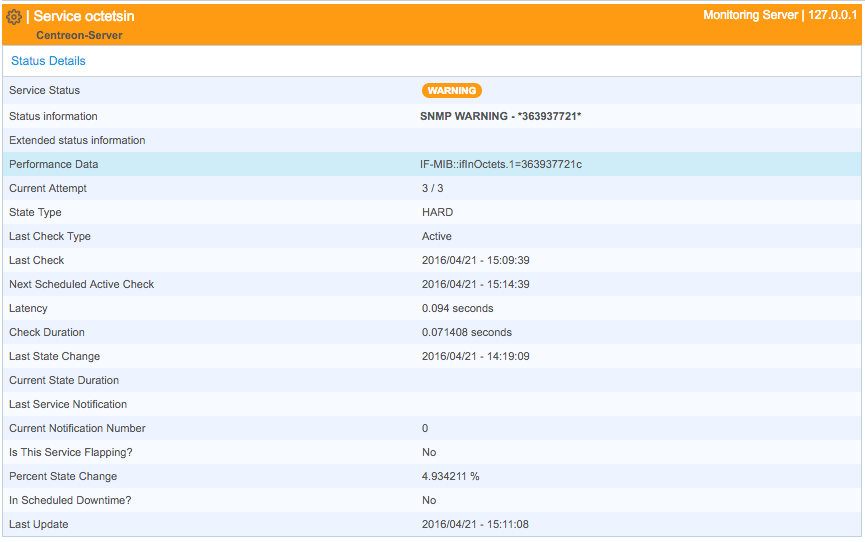
\includegraphics[width=150mm,scale=1]{imagens/WarningService.png}
 \caption{Serviço com alerta "Warning"}
 \label{fig:warning}
\end{figure}

No exemplo acima, na criação do comando para este serviço, definiu-se um valor, que caso fosse ultrapassado, lançaria um alerta de "warning". Neste caso foi na quantidade de octetos que entram na interface 1.

\newpage
Quando um serviço corre sem qualquer problema, obtém-se uma mensagem de "ok":

\begin{figure}[!htb]
\center
 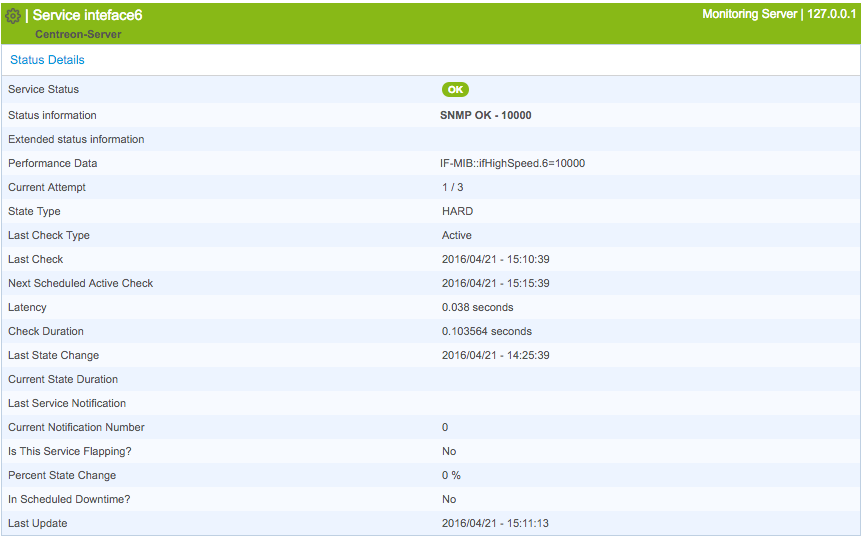
\includegraphics[width=150mm,scale=1]{imagens/OKService.png}
 \caption{Serviço com alerta "OK"}
 \label{fig:ok}
\end{figure}

É possível ainda em cada serviço, ter um gráfico com o histórico do estado do serviço, ao longo de um determinado intervalo de tempo:

\begin{figure}[!htb]
\center
 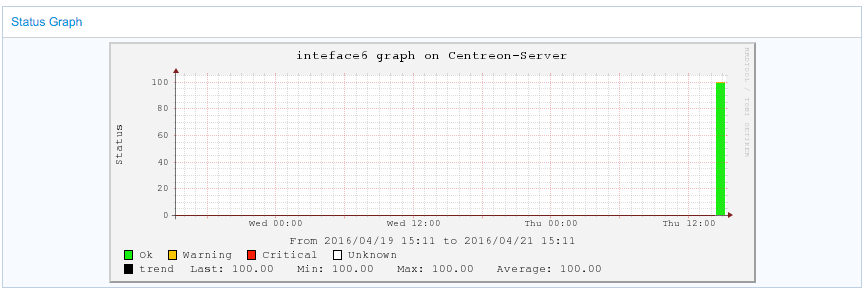
\includegraphics[width=150mm,scale=1]{imagens/OKGraph.png}
 \caption{Gráfico do serviço com alerta "OK"}
 \label{fig:grafico}
\end{figure}

\newpage
\section{Datadog}

Datadog é também um sistema de monitorização. Foi utilizado para monitorizar a máquina que contém o ambiente Docker. Para isso, foi instalado na máquina, através do Rancher:

\begin{figure}[!htb]
\center
 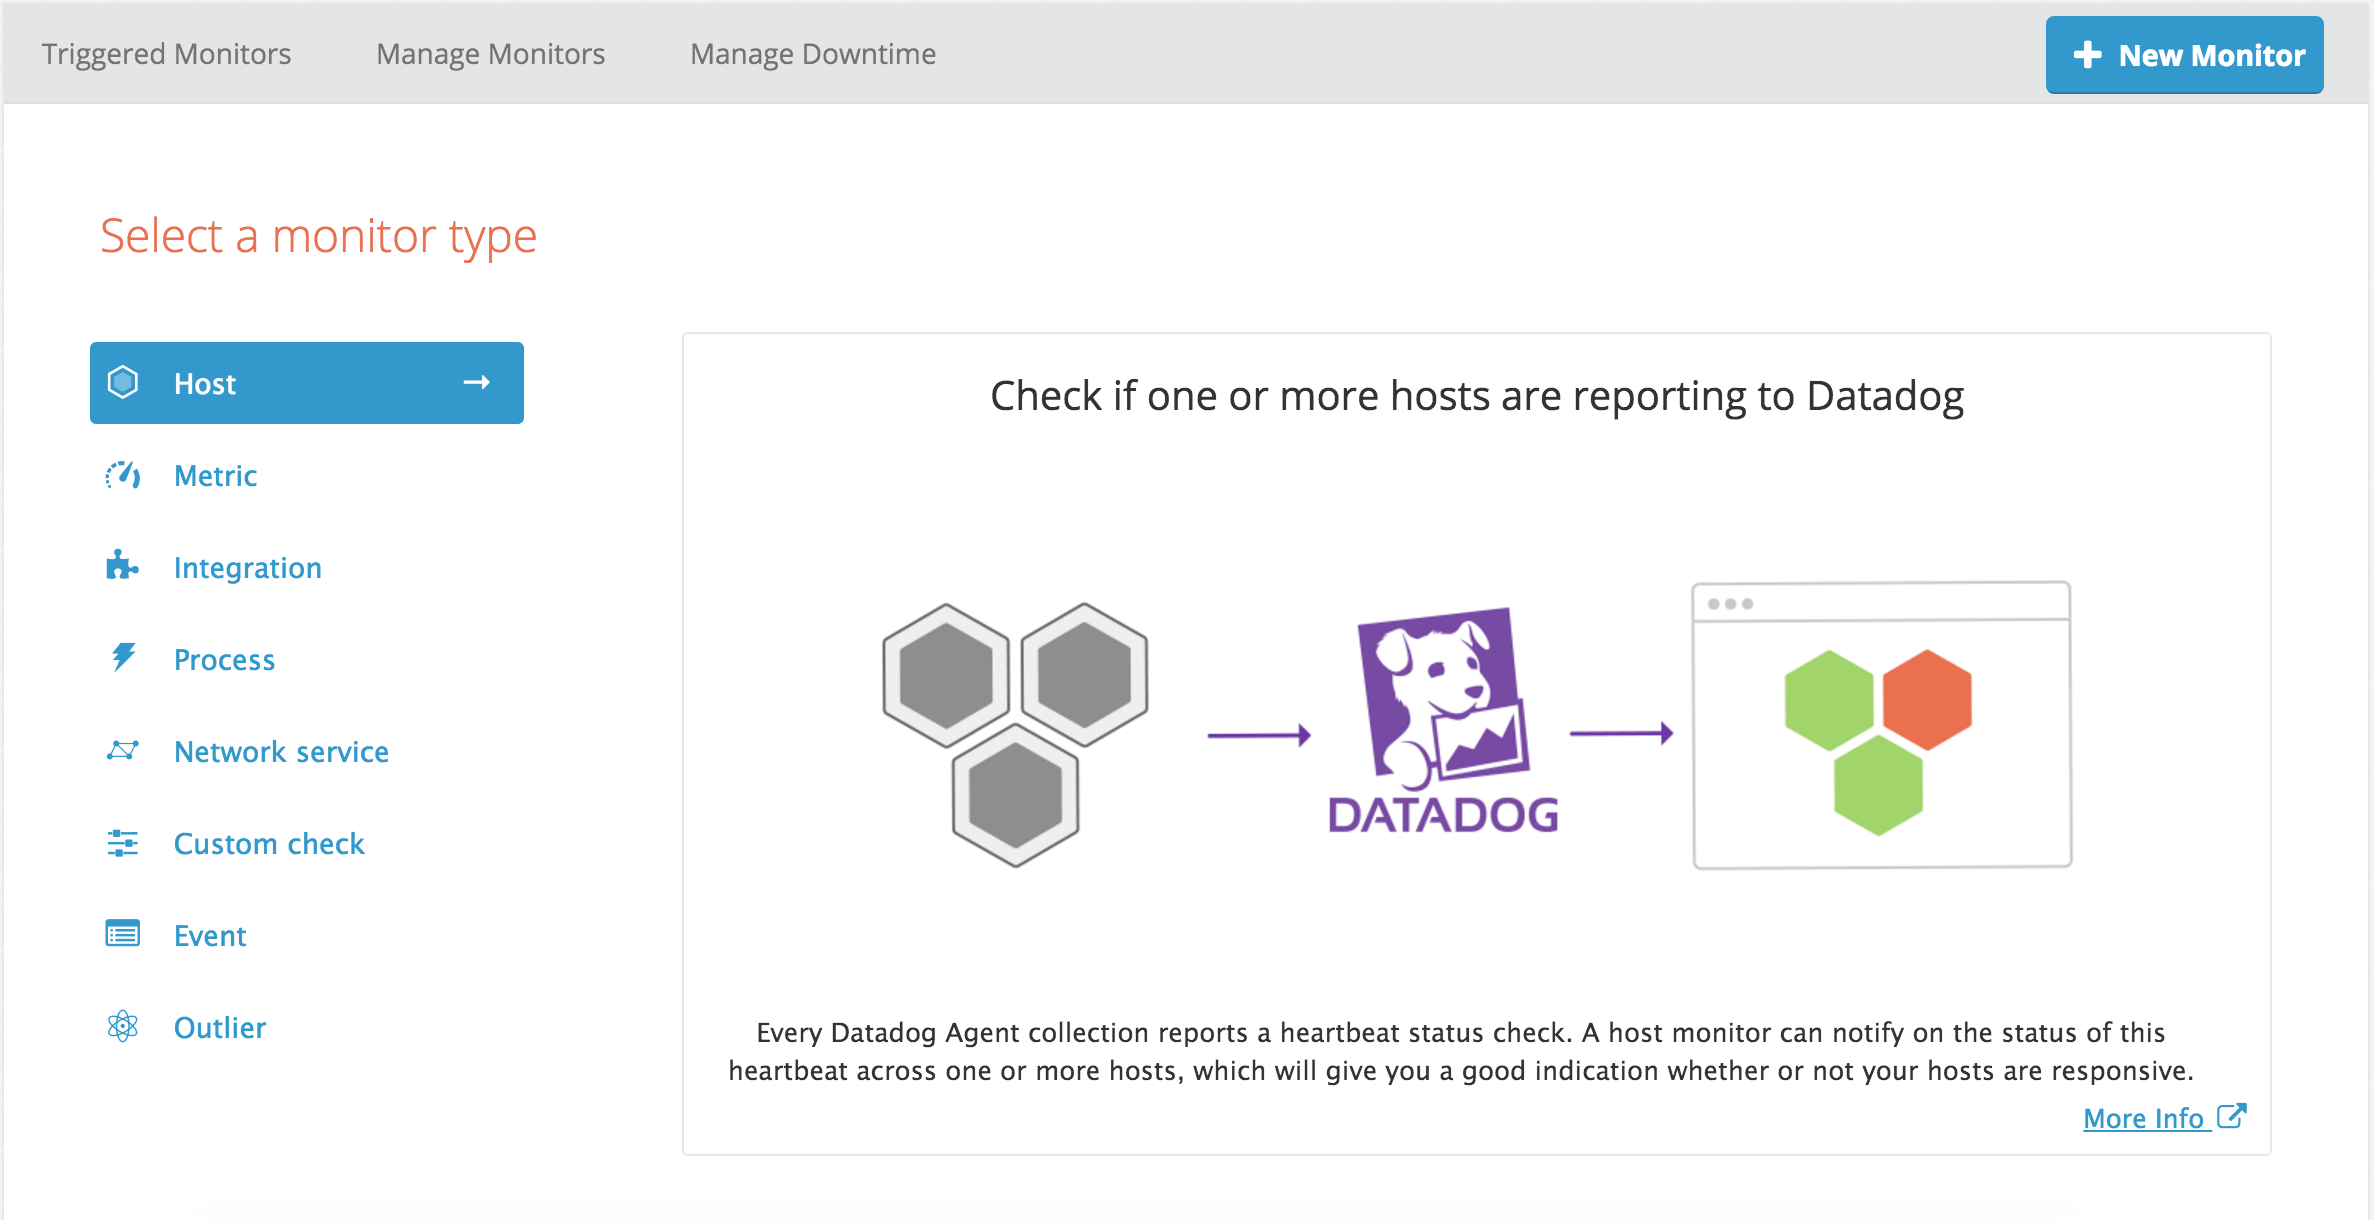
\includegraphics[width=150mm,scale=1]{imagens/select_monitor_to_trigger.png}
 \caption{Seleção do sistema a ser monitorizado}
 \label{fig:select}
\end{figure}

\begin{figure}[!htb]
\center
 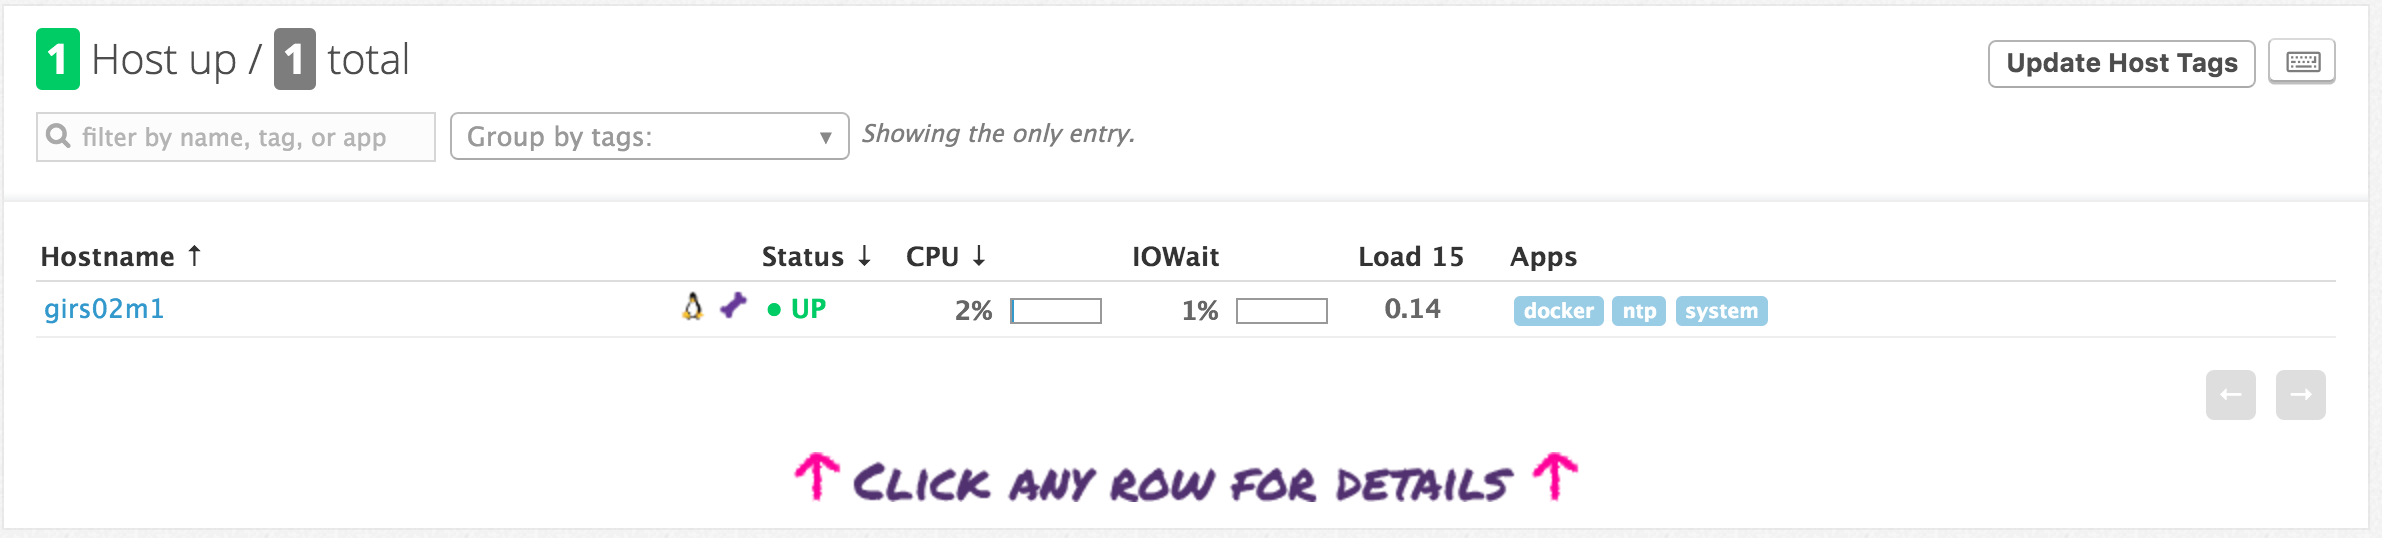
\includegraphics[width=150mm,scale=1]{imagens/hosts.png}
 \caption{Host que está a ser monitorizado}
 \label{fig:hots}
\end{figure}

Foi selecionada a máquina "girs02m1", para ser monitorizada. Quando é selecionada, é apresentada uma dashboard onde é possível ver os eventos que ocorreram na mesma, num intervalo de tempo.

\begin{figure}[!htb]
\center
 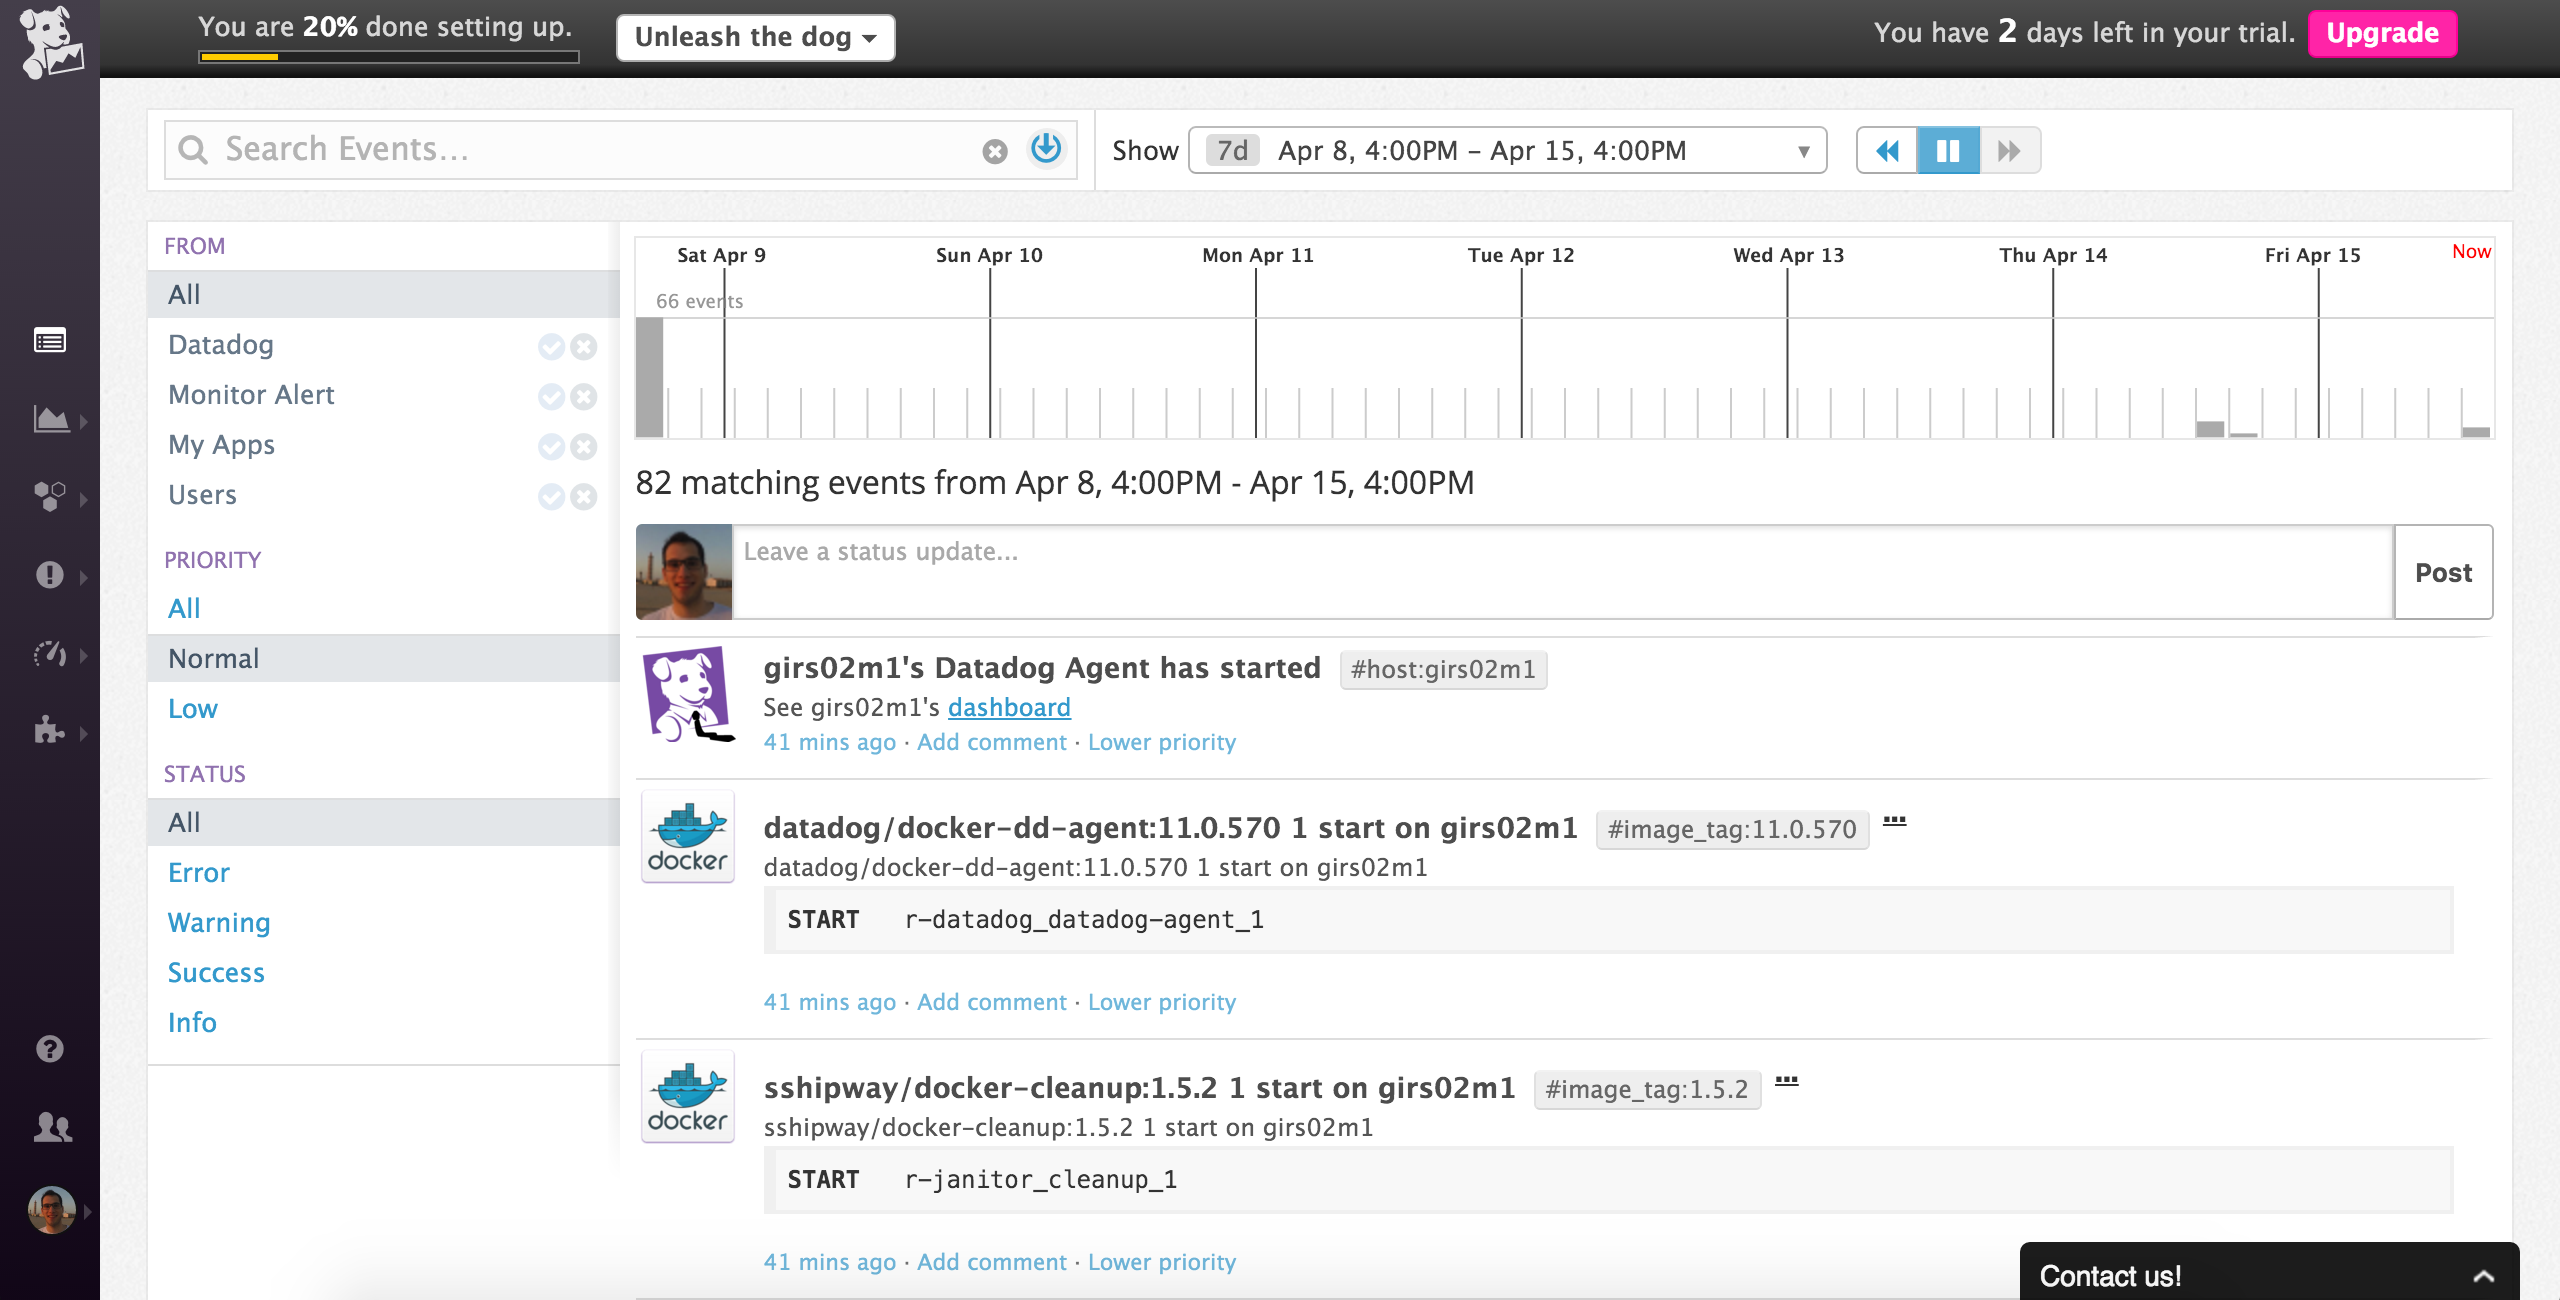
\includegraphics[width=150mm,scale=1]{imagens/datadog_dashboard.png}
 \caption{Dashboard Datadog}
 \label{fig:dashboard}
\end{figure}
\newpage

Um outro ponto, bastante relevante desta plataforma, são os gráficos disponibilizados com informação relativamente à memória utilizada, espaço ocupado, número de containers a funcionar, utilização do cpu, entre outros:

\begin{figure}[!htb]
\centering
\begin{minipage}{.5\textwidth}
  \centering
  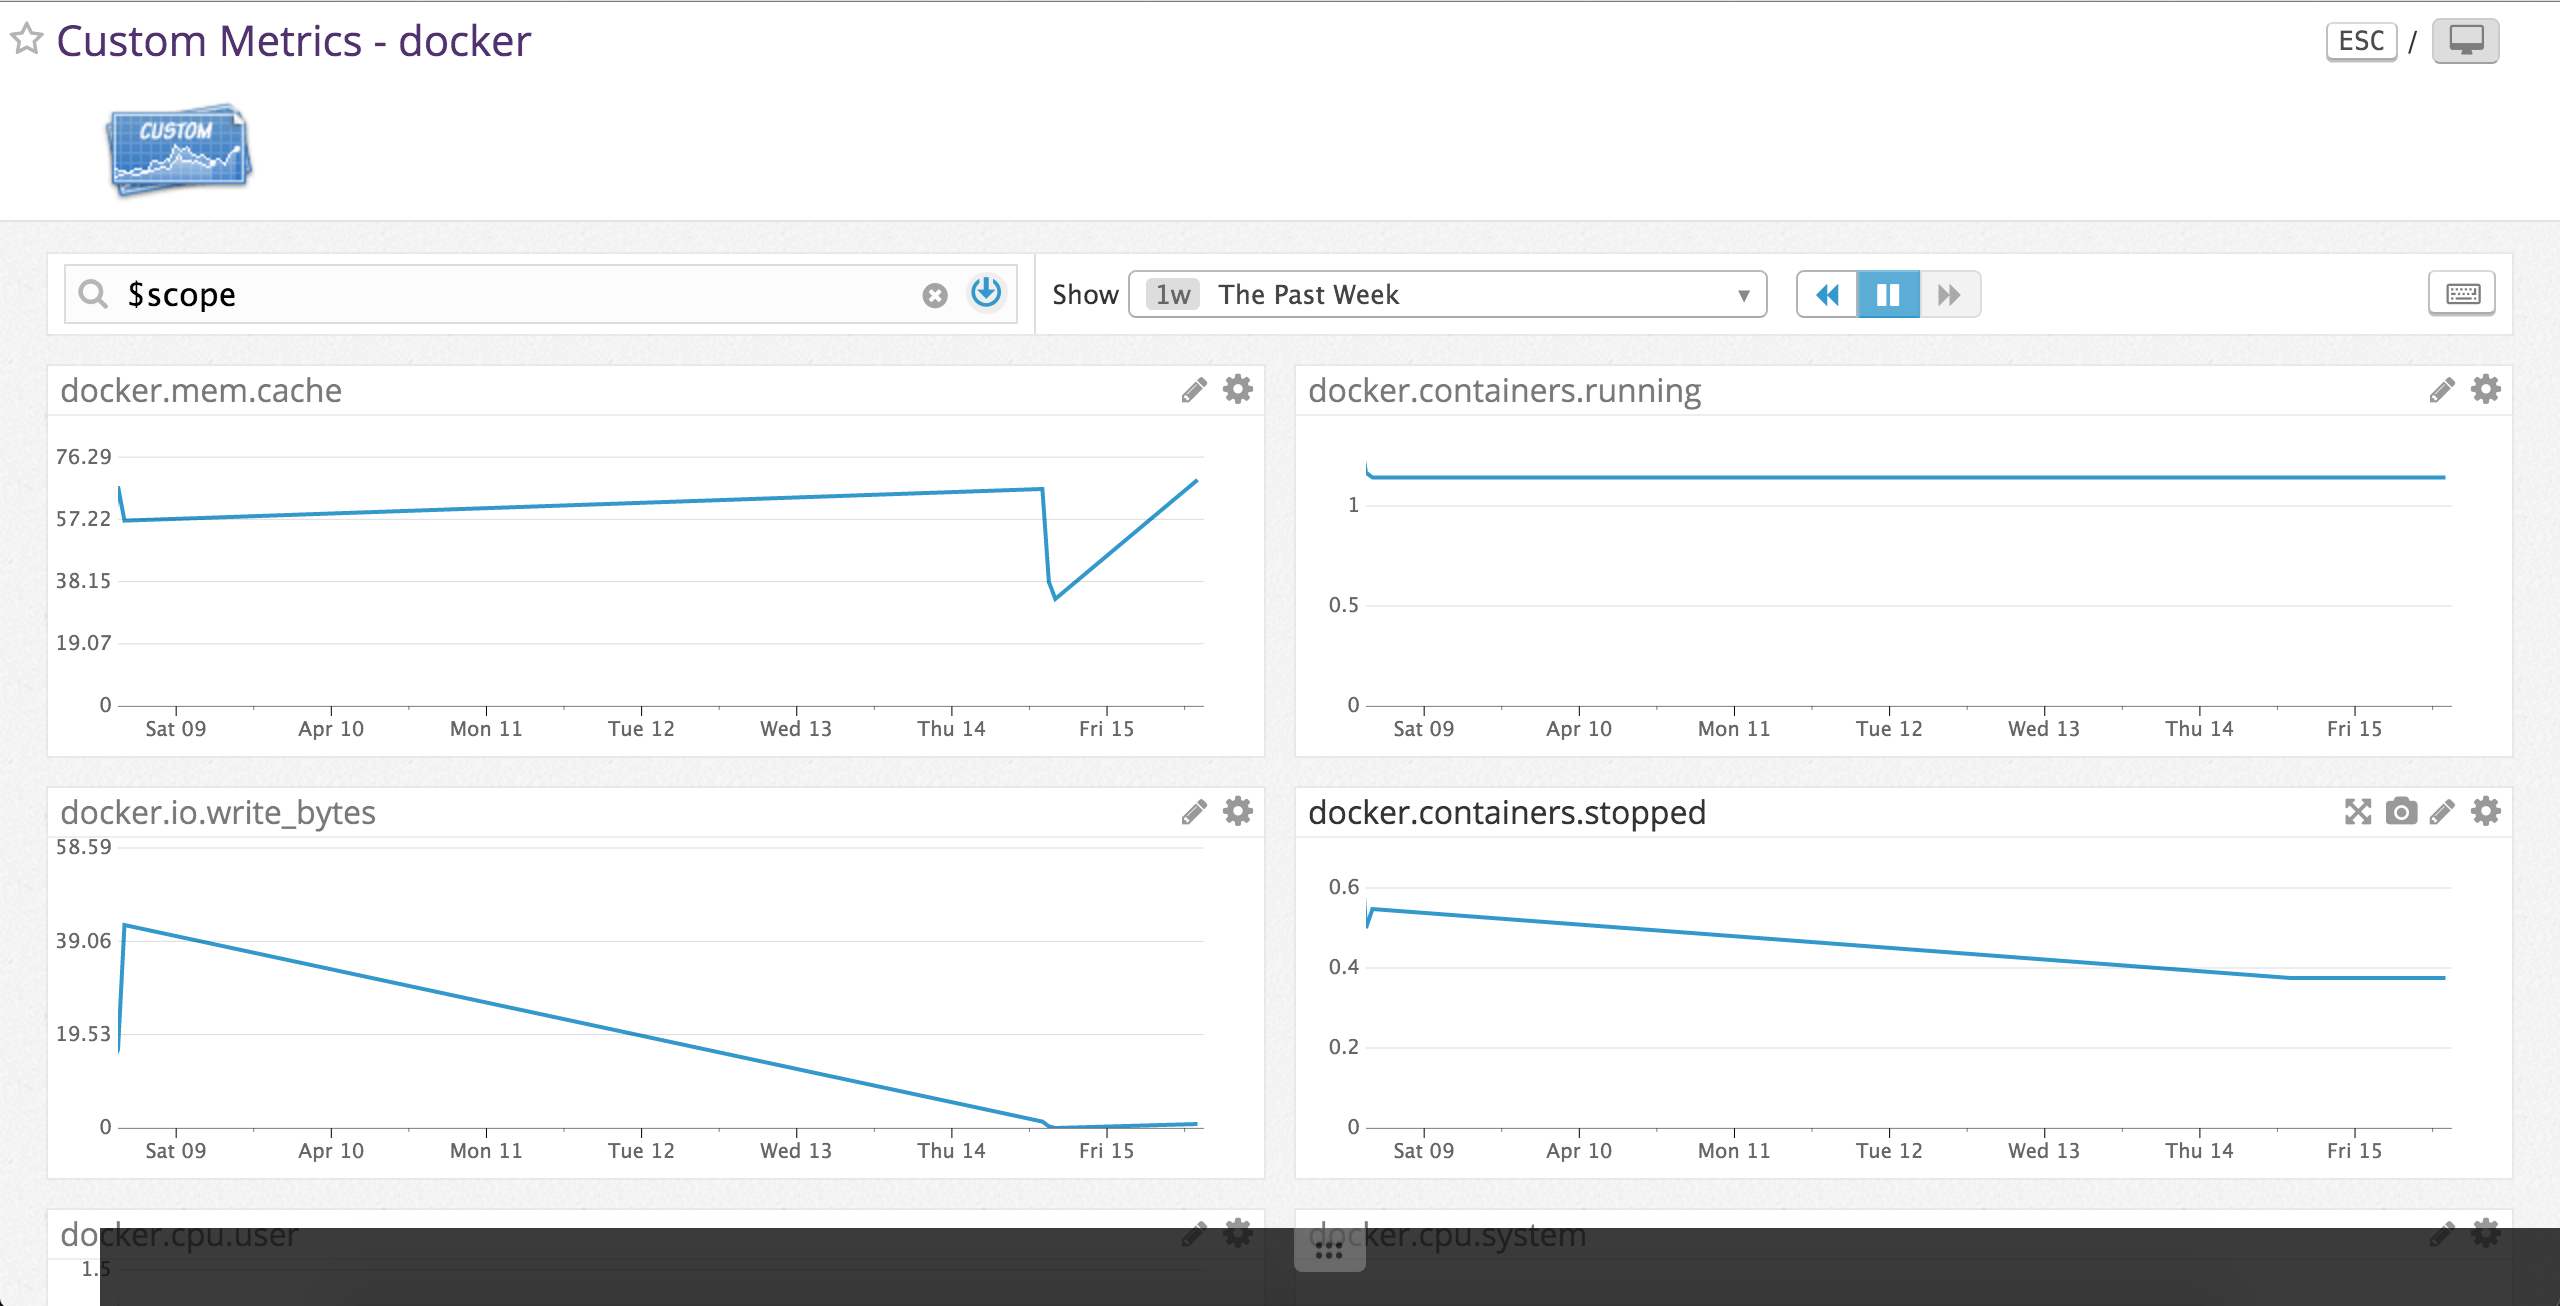
\includegraphics[width=65mm,scale=1]{imagens/datadog_metrics_docker.png}
  \captionof{figure}{Gráficos Métricas I}
  \label{fig:metricas1}
\end{minipage}%
\begin{minipage}{.5\textwidth}
  \centering
  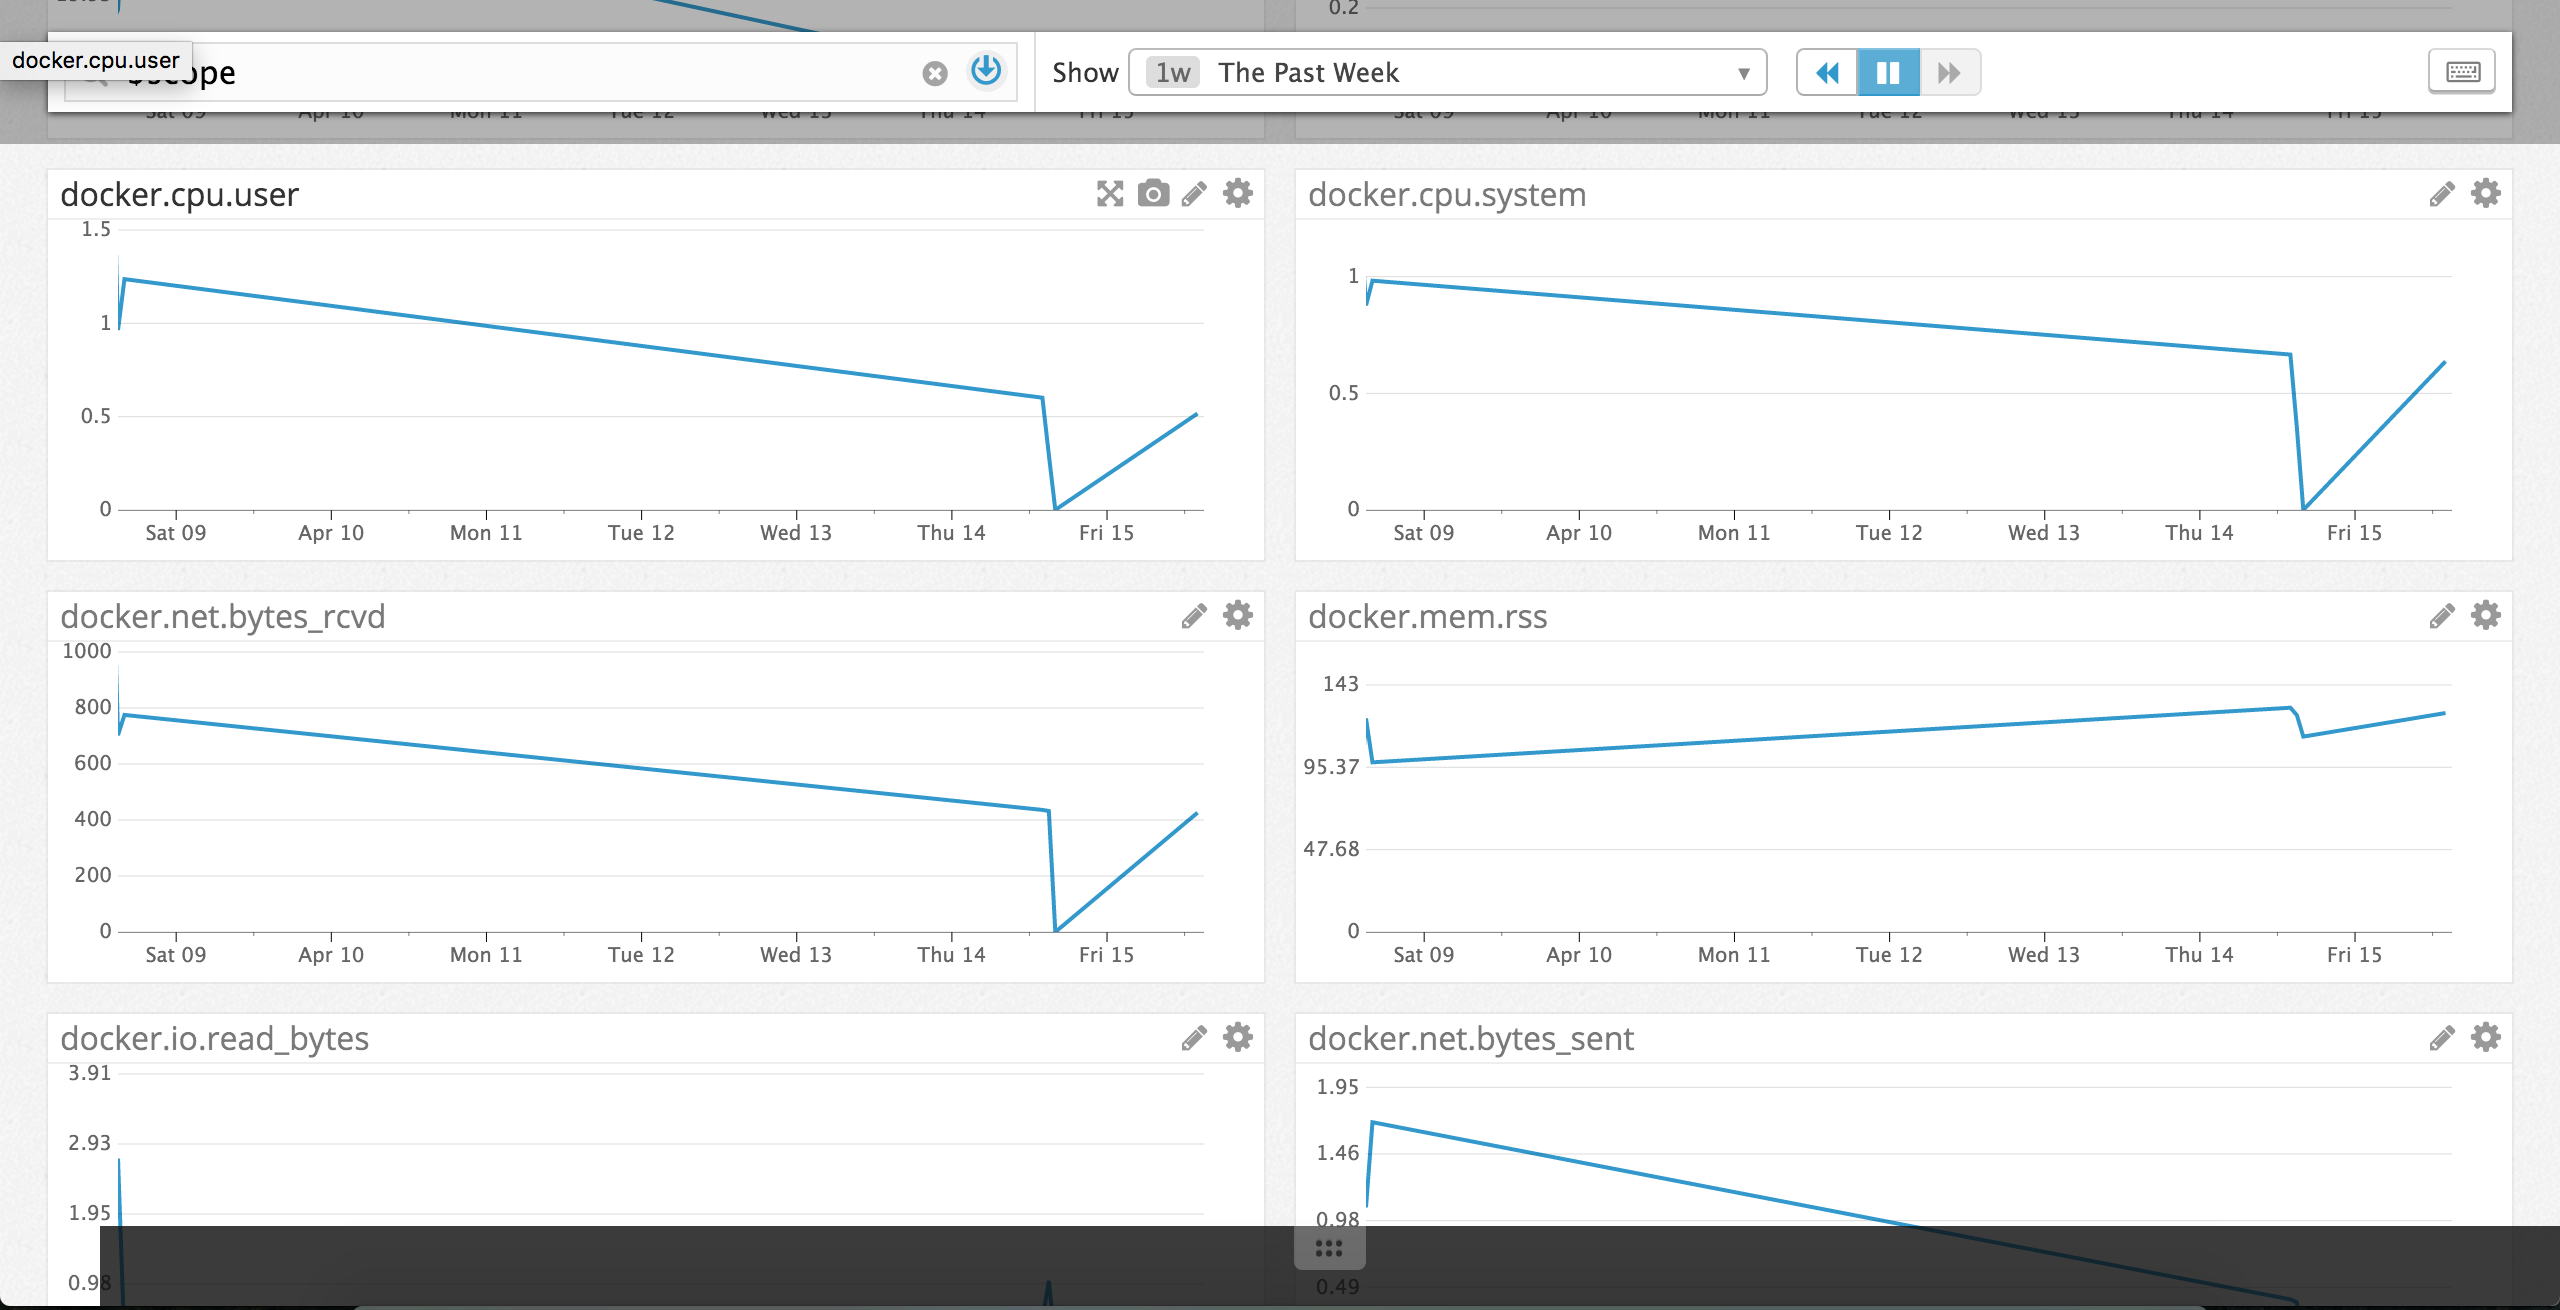
\includegraphics[width=65mm,scale=1]{imagens/datadog_metrics_docker2.png}
  \captionof{figure}{Gráficos Métricas II}
  \label{fig:metricas2}
\end{minipage}
\end{figure}

\newpage

\section{Load balancer}

\begin{figure}[!htb]
\center
 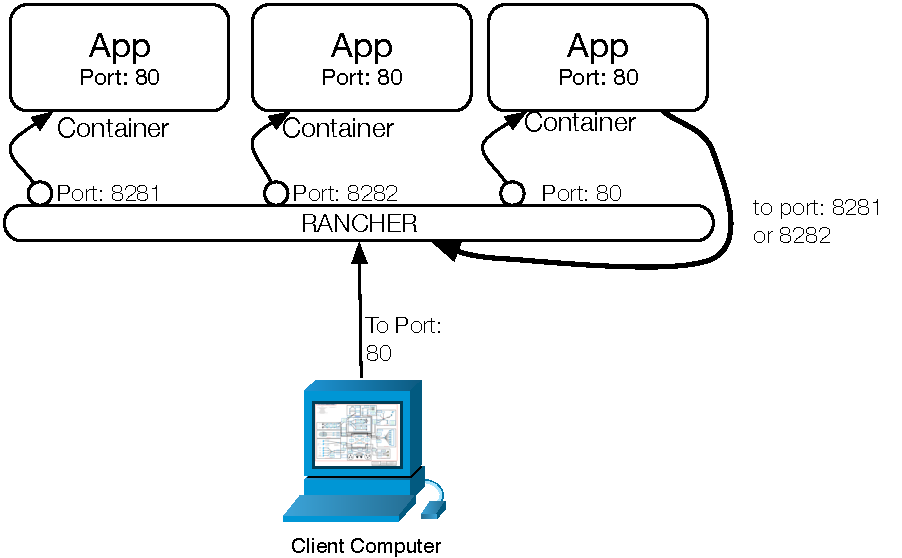
\includegraphics[width=100mm,scale=1]{imagens/simple_load_balancer.pdf}
 \caption{LoadBalancer Simples com NGINX}
 \label{fig:dashboard}
\end{figure}

A nossa solução para fazer o balanceamento passou pela construção de uma Stack com 3 containers, dois que têm a mesma aplicação a correr na porta 80 mapeada para portos diferentes do Host e outro container que tem NGINX à escuta também num porto diferente.

Para criar a aplicação fez-se as seguintes ações:

\shellcmd{apt-get update}
\shellcmd{apt-get install -y apache2 php5 libapache2-mod-php5 vim}
\shellcmd{cd /var/www/html/}
\shellcmd{rm index.html}
\shellcmd{vim index.php}
\shellcmd{service apache2 start}

\begin{lstlisting}
<?php

$start_script = gettimeofday();

const INTERVAL = 0.04;
$dummy = 0;
$cycles = 1000;

$rand = rand(50, 100);
for($j = 0; $j < $rand; $j++){
  $start = gettimeofday();
  for($i=0; $i<$cycles; $i++){
    $dummy += $i*$i;
  }
  $stop = gettimeofday();

  $spentTime = ($stop["sec"]-$start["sec"]) +
   ($stop["usec"]-$start["usec"]) / 1000000.0;
  $cycles = ($cycles / $spentTime) * ($target_load / 100.0) * INTERVAL;
  usleep((1000000 * INTERVAL - $spentTime*1000000));
}

$stop_script = gettimeofday();

echo "<pre>";
echo "start: ";
print_r($start_script);
echo "\n stop:";
print_r($stop_script);
echo "\n done! \n";
echo "hostname: ";
echo gethostname();
echo "</pre>";

?>
\end{lstlisting}

\subsection{Nginx como Load Balancer}

Ao aceder pelo seu computador, para a porta do LoadBalancer, este irá reencaminhar o pedido para outro container e pode seguir várias políticas para fazer este reencaminhamento:

\subsubsection{Por defeito}
Por defeito o algoritmo de balanceamento usado é "round-robin", todos os pedidos são processados independentemente da carga e são redirecionados de igual forma para os containers disponíveis na configuração\href{http://nginx.org/en/docs/http/load_balancing.html}.

Uma configuração possível para a nossa solução:

\begin{lstlisting}
upstream 192.168.215.20  {
  server 192.168.215.20:8281;
  server 192.168.215.20:8282;
}

server {
  location / {
    proxy_pass  http://192.168.215.20;
  }
}
\end{lstlisting}

\subsubsection{Least connected}
Outra forma de fazer load balancing é com o least-connected (menos-conectado). Este permite controlar a carga nas instâncias de forma justa em que alguns dos pedidos levam mais tempo para serem concluídos.

Com este método de balanceamento, Nginx vai tentar não sobrecarregar um servidor que esteja ocupados com pedidos excessivos, distribuindo os novos pedidos para um servidor que esteja menos ocupado.

Uma configuração possível para a nossa solução:

\begin{lstlisting}
upstream 192.168.215.20 {
	least_conn;
    server 192.168.215.20:8281;
    server 192.168.215.20:8282;
}

server {
  location / {
    proxy_pass  http://192.168.215.20;
  }
}
\end{lstlisting}

\subsubsection{Session persistence}
Com round-robin ou least-connected, a sessão do cliente pode ser destruída se não existir um meio de persistência destas. Não há garantia de que o mesmo cliente será sempre direcionado para o mesmo servidor.

Se existir necessidade de permanecer o cliente num dado servidor para garantir a persistência da sessão, é necessário usar o mecanismo ip-hash de balanceamento de carga.

Com este mecanismo, o IP do cliente é usado como chave da tabela de hashing para determinar qual é servidor que deve ser selecionado para os pedidos dos clientes. Este método garante que os pedidos do mesmo cliente sejam sempre direcionados para o mesmo servidor exceto quando o servidor já não está disponível.

Uma configuração possível para a nossa solução:

\begin{lstlisting}
upstream 192.168.215.20  {
	ip_hash;
    server 192.168.215.20:8281;
    server 192.168.215.20:8282;
}

server {
  location / {
    proxy_pass  http://192.168.215.20;
  }
}
\end{lstlisting}

\subsubsection{Weight}
Esta opção permite enviar os utilizadores para os servidores com mais precisão e alocar peso com peso certo para determinadas máquinas.

Nginx permite que se redirecione o tráfego para uma máquina específica com mais proporção ou com menos proporção.

Uma configuração possível para a nossa solução:

\begin{lstlisting}
upstream 192.168.215.20  {
  server 192.168.215.20:8281 weight=1;
  server 192.168.215.20:8282 weight=2;
}

server {
  location / {
    proxy_pass  http://192.168.215.20;
  }
}
\end{lstlisting}

Por defeito, o peso é 1. Com o peso de 2, o container na porta 8282 irá receber duas vezes mais tráfego do que o container no porto 8281.

\subsubsection{Max Fails}

De acordo \footnote{https://www.digitalocean.com/community/tutorials/how-to-set-up-nginx-load-balancing} com a configuração por defeito do round robin, o nginx irá continuar a enviar pedidos para o container, mesmo que o container/servidor não estejam a responder. Com a diretiva max fails é possível prevenir automaticamente detetando servidor que não estejam a responder por um tempo determinado.

Existem dois comandos que podem ser usados: max\_fails e fail\_timeout. Max fails refere-se ao número máximo de tentativas falhadas ao tentar conectar-se ao servidor antes de se considerar inativo. Fail\_timeout é o tempo que é necessário para considerar um servidor intativo. Quando esse tempo expirar, irá ser eliminado da tabela, quando voltar a estar disponível, irá voltar a estar na tabela.

Uma configuração possível para a nossa solução:

\begin{lstlisting}
upstream 192.168.215.20  {
    server 192.168.215.20:8281 max_fails=3  fail_timeout=15s;
    server 192.168.215.20:8282 weight=2;
}

server {
  location / {
    proxy_pass  http://192.168.215.20;
  }
}
\end{lstlisting}

\subsection{Load balancing tendo em conta a carga do CPU dos containers}

Pretende-se usando SNMP obter a carga de cada container em tempo real de forma a enviar o pedido para o container com a carga de CPU menor.


\subsubsection{Carga de CPU de um container}

Para obter a carga do CPU de um container foi usado um script bash para obter a informação sobre o estado dos containers.  É feito o parse da carga de CPU dada pelo comando \textbf{docker stats}.

O container é identificado pela porta que ele usa no host, que neste caso é a 8281.

\begin{lstlisting}
#!/usr/bin/env bash
PORTS=$(docker ps | grep ">80/tcp" | grep "0.0.0.0:8281" \
 | awk '/ /{print $10}' | sed -r 's/[0.0.0.0:]+//g' \
  | sed -r 's/->8\/tcp//') # ports
CONTAINER=$( docker ps | grep ">80/tcp" | grep "0.0.0.0:8281"\
 | awk '/ /{print $1}') # containers
CPU_CONTAINER=$(docker stats --no-stream $CONTAINER \
 | awk '/ /{print $2}' | grep "%" | sed -r 's/%//')
echo ${CPU_CONTAINER}
\end{lstlisting}

\subsubsection{SNMP}

Para que o snmp tivesse acesso ao daemon do Docker foi necessário executar o seguinte comando:

\shellcmd{sudo usermod -aG docker snmp}
\shellcmd{sudo service snmpd restart}

Já a configuração do SNMP foi normal, usando a versão 3, foi criado um utilizador e uma password para o mesmo:

\begin{lstlisting}
createUser bootstrap MD5 temp_password DES
\end{lstlisting}

Foi também necessário colocar o SNMP disponível em todas as interfaces:

\begin{lstlisting}
agentAddress udp:161,udp6:[::1]:161
\end{lstlisting}

Na secção "EXTENDING THE AGENT", foi colocado dois comandos, um "app1" e outro "app2" que serão encarregados por retornar a percentagem de CPU usada pelo container.

\begin{lstlisting}
 extend    app1    /bin/sh /path/to/app1.sh
 extend    app2    /bin/sh /path/to/app2.sh 
\end{lstlisting}

Usando então um snmpget é possível então obter a percentagem pretendida.

\shellcmd{snmpget -v 3 -u authOnlyUser -l authPriv -a MD5 -A \
temp\_password -x DES -X temp\_password IP.IP.IP.IP \
 'NET-SNMP-EXTEND-MIB::nsExtendOutputFull."app1"'}

\subsubsection{Obtendo a carga dos containers usando C}

Usando o popen executa-se o comando SNMP, o código apresentado no relatório não é o completo.

\begin{lstlisting}

/* Open the command for reading. */
  fp = popen("snmpget -v 3 -u authOnlyUser -l authPriv -a MD5
   -A temp_password -x DES -X temp_password IP.IP.IP.IP
    'NET-SNMP-EXTEND-MIB::nsExtendOutputFull.\"app1\"'", "r");
  if (fp == NULL) {
    printf("Failed to run command\n" );
    exit(1);
  }

\end{lstlisting}

Depois faz-se o parse da string obtida para inteiro:

\begin{lstlisting}
char app1[10];

  int pos = 57;
  int i = pos;

  while(path[i]!=0){
    app1[i-pos] = path[i];
    i = i + 1;
  }

  int app1_val = parseToInt(app1, 0, i-pos-1);
\end{lstlisting}


De seguida faz-se a comparação.

\newpage

\subsubsection{Costumização do NGINX}

\begin{figure}[!htb]
\center
 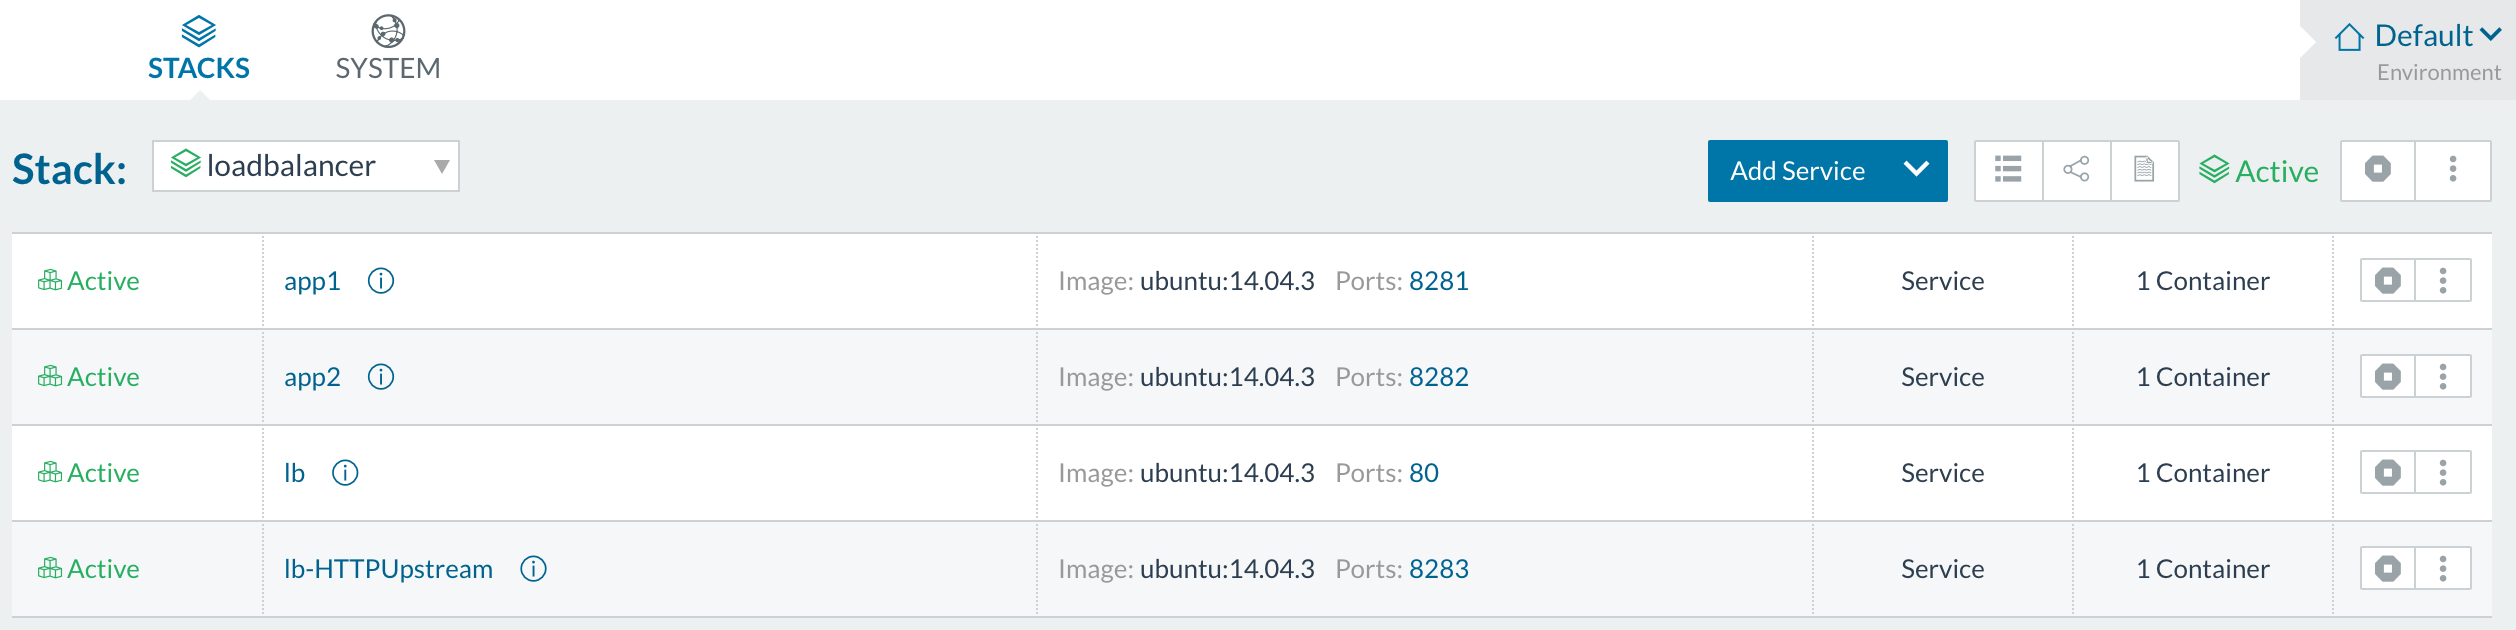
\includegraphics[width=130mm,scale=1]{imagens/app-list.png}
 \caption{Solução final}
 \label{fig:dashboard}
\end{figure}

Na porta 80 estará o NGINX modificado que tem em consideração a carga do CPU de cada container. Na porta 8281 estará a app1, na porta 8282 a app2 e na porta 8283 um loadbalancer NGINX não modificado.

Para se realizar a costumização do NGINX foi inicialmente instalado as bibliotecas necessárias  e feito o git clone do repositório do NGINX.

\shellcmd{apt-get update}
\shellcmd{apt-get install -y git vim build-essential libc6 libpcre3 libpcre3-dev
libpcrecpp0 libssl0.9.8 libssl-dev zlib1g zlib1g-dev lsb-base openssl libssl-dev
libgeoip1 libgeoip-dev  google-perftools libgoogle-perftools-dev libperl-dev
libgd2-xpm-dev libatomic-ops-dev libxml2-dev libxslt1-dev python-dev 
snmp snmp-mibs-downloader}
\shellcmd{cd /}
\shellcmd{git clone https://github.com/nginx/nginx.git}
\shellcmd{vim nginx/src/http/ngx\_http\_upstream\_round\_robin.c 
\# mais em baixo estará focada a alteração do código}
\shellcmd{cd nginx}
\shellcmd{./auto/configure 
--sbin-path=/usr/local/nginx/nginx  
--conf-path=/etc/nginx/nginx.conf 
--pid-path=/var/run/nginx.pid 
--with-debug  --with-select\_module 
--with-poll\_module 
--error-log-path=/var/log/nginx/error.log 
--http-log-path=/var/log/nginx/access.log}
\shellcmd{make \&\& make install}
\shellcmd{mkdir /etc/nginx/sites-available}
\shellcmd{mkdir /etc/nginx/sites-enabled}
\shellcmd{vim /etc/nginx/nginx.conf \# add in http 
section: include /etc/nginx/sites-available/*;}
\shellcmd{vim /etc/nginx/sites-available/default}

\begin{lstlisting}
upstream 192.168.215.20  {
  server 192.168.215.20:8281;
  server 192.168.215.20:8282;
}

server {
  location / {
    proxy_pass  http://192.168.215.20;
  }
}
\end{lstlisting}

Para iniciar e terminar o NGINX, é usado os seguintes comandos:

\shellcmd{/usr/local/nginx/nginx \# start NGINX}
\shellcmd{kill -QUIT \$\( cat /var/run/nginx.pid \) \# stop NGINX}

No container irá existir um daemon que estará sempre em execução e o seu trabalho será obter os a carga dos containers por SNMP e guardar numa variável numa zona partilhada para que o NGINX depois consiga aceder a essa variável sem ter de esperar pela resposta do SNMP. 

Durante o nosso desenvolvimento também foi possível perceber que o SNMP responde sempre da mesma forma durante 3 ou 4 segundos, aparentemente fazendo cache dos pedidos efetuados, dificulta assim ter dados sobre o CPU atualizados ao segundo, sendo que o ganho terá de ser considerado para intervalos superiores a este.

No ficheiro \textbf{nginx/src/http/ngx\_http\_upstream\_round\_robin.c} foi  modificada a função \textbf{ngx\_http\_upstream\_get\_peer} para obter os dados guardados na zona partilhada:

\begin{lstlisting}
static ngx_http_upstream_rr_peer_t *
ngx_http_upstream_get_peer(ngx_http_upstream_rr_peer_data_t *rrp)
{
    time_t                        now;
    uintptr_t                     m;
    ngx_int_t                     total;
    ngx_uint_t                    i, n, p;
    ngx_http_upstream_rr_peer_t  *peer, *best;

    now = ngx_time();

    best = NULL;
    total = 0;

#if (NGX_SUPPRESS_WARN)
    p = 0;
#endif
    // https://www.cs.cf.ac.uk/Dave/C/node27.html

    int shmid;
    key_t key;
    int *shm, *s;

    /*
     * We need to get the segment named
     * "5678", created by the server.
     */
    key = 5678;

    /*
     * Locate the segment.
     */
    if ((shmid = shmget(key, SHMSZ, 0666)) < 0) {
        perror("shmget");
        exit(1);
    }

    /*
     * Now we attach the segment to our data space.
     */
    if ((shm = shmat(shmid, NULL, 0)) == (int *) -1) {
        perror("shmat");
        exit(1);
    }

    /*
     * Now read what the server put in the memory.
     */
     s = shm;

     ngx_uint_t ix = *s;

    for (peer = rrp->peers->peer, i = 0;
         peer;
         peer = peer->next, i++)
    {
        if (best == NULL || i==ix) {
            best = peer;
            p = i;
            break;
        }
    }

    rrp->current = best;

    n = p / (8 * sizeof(uintptr_t));
    m = (uintptr_t) 1 << p % (8 * sizeof(uintptr_t));

    rrp->tried[n] |= m;

    best->current_weight -= total;

    if (now - best->checked > best->fail_timeout) {
        best->checked = now;
    }

    return best;
}
\end{lstlisting}

Para o daemon responsável por obter a informação sobre os containers através de SNMP foi elaborado o seguinte código:

\begin{lstlisting}
#include <stdio.h>
#include <stdlib.h>
#include <ctype.h>
#include <sys/types.h>
#include <sys/ipc.h>
#include <sys/shm.h>
#include <stdio.h>

#define SHMSZ     27

// gcc get-snmp.c -o server-get-snmp.out && ./server-get-snmp.out &> output &
// ps aux | grep "get"

int parseToInt(const char* s, int start, int stop) {
    unsigned long long int m = 1;
    int ret = 0;
    int i = stop;

    for (; i >= start; i--) {
      if(isdigit(s[i])){
        ret += (s[i] - '0') * m;
        m *= 10;
      }
    }

    return ret;
}

int main(int argc, char const *argv[]) {
  // https://www.cs.cf.ac.uk/Dave/C/node27.html

  int shmid;
  key_t key;
  int *shm, *s;

  /*
   * We'll name our shared memory segment
   * "5678".
   */
  key = 5678;

  /*
   * Create the segment.
   */
  if ((shmid = shmget(key, SHMSZ, IPC_CREAT | 0666)) < 0) {
      perror("shmget");
      exit(1);
  }

  /*
   * Now we attach the segment to our data space.
   */
  if ((shm = shmat(shmid, NULL, 0)) == (int *) -1) {
      perror("shmat");
      exit(1);
  }

  /*
   * Now put some things into the memory for the
   * other process to read.
   */
  s = shm;

  while(1){
    printf("Getting app 1 CPU status....\n");

    FILE *fp;
    char path[1035] = "";

    /* Open the command for reading. */
    fp = popen("snmpget -v 3 -u authOnlyUser -l 
authPriv -a MD5 -A temp_password -x DES -X 
temp_password 192.168.215.20 
'NET-SNMP-EXTEND-MIB::nsExtendOutputFull.\"app1\"'", "r");
    if (fp == NULL) {
      printf("Failed to run command\n" );
      exit(1);
    }

    /* Read the output a line at a time - output it. */
    while (fgets(path, sizeof(path)-1, fp) != NULL) {
      printf("%s", path);
    }

    /* close */
    pclose(fp);

    // parse what we need
    char app1[10];

    int pos = 57;
    int i = pos;

    while(path[i]!=0){
      app1[i-pos] = path[i];
      i = i + 1;
    }

    int app1_val = parseToInt(app1, 0, i-pos-1);

    printf("VALUE APP1: %d (%%)\n", app1_val);

    printf("Getting app 2 CPU status....\n");
    FILE *fp2;
    char path2[1035];

    /* Open the command for reading. */
    fp2 = popen("snmpget -v 3 -u authOnlyUser -l authPriv
-a MD5 -A temp_password -x DES -X 
temp_password 192.168.215.20 
'NET-SNMP-EXTEND-MIB::nsExtendOutputFull.\"app2\"'", "r");
    if (fp2 == NULL) {
      printf("Failed to run command\n" );
      exit(1);
    }

    /* Read the output a line at a time - output it. */
    while (fgets(path2, sizeof(path2)-1, fp2) != NULL) {
      printf("%s", path2);
    }

    /* close */
    pclose(fp2);

    // parse what we need
    char app2[10];

    i = pos;

    while(path[i]!=0){
      app1[i-pos] = path[i];
      i = i + 1;
    }

    int app2_val = parseToInt(app2, 0, i-pos-1);

    printf("VALUE APP2: %d (%%)\n", app2_val);

    int ix = 0;

    if(app1_val>app2_val){
        ix = 1;
    }

    *s = ix;
    sleep(4);
  }

  return 0;
}
\end{lstlisting}

\newpage
\subsubsection{Benchmark do NGINX comparando com o normal}

Usando o Apache Benchmark, sabendo que cada pedido demora em média 5 a 6 segundos, foram realizados 500 pedidos com concorrência de 30 pedidos.

% Please add the following required packages to your document preamble:
% \usepackage[normalem]{ulem}
% \useunder{\uline}{\ul}{}
\begin{table}[!htb]
\centering
\centering
\caption{Comparação entre testes}
\label{my-label}
\resizebox{\textwidth}{!}{
\begin{tabular}{llllllllll}
\hline
\multicolumn{1}{|l|}{}                    & \multicolumn{1}{l|}{\textbf{Teste 1}} & \multicolumn{1}{l|}{\textbf{Teste 2}} & \multicolumn{1}{l|}{\textbf{Teste 3}} & \multicolumn{1}{l|}{\textbf{Teste 4}} & \multicolumn{1}{l|}{\textbf{Teste 5}} & \multicolumn{1}{l|}{\textbf{Teste 6}} & \multicolumn{1}{l|}{\textbf{Teste 7}} & \multicolumn{1}{l|}{\textbf{Teste 8}} & \multicolumn{1}{l|}{{\ul \textit{\textbf{Média}}}} \\ \hline
\multicolumn{1}{|l|}{\textbf{Normal}}     & \multicolumn{1}{l|}{161.498}          & \multicolumn{1}{l|}{192.892}          & \multicolumn{1}{l|}{181.070}          & \multicolumn{1}{l|}{189.433}          & \multicolumn{1}{l|}{173.298}          & \multicolumn{1}{l|}{171.766}          & \multicolumn{1}{l|}{176.420}          & \multicolumn{1}{l|}{185.243}          & \multicolumn{1}{l|}{178,952}                       \\ \hline
\multicolumn{1}{|l|}{\textbf{Modificado}} & \multicolumn{1}{l|}{107.544}          & \multicolumn{1}{l|}{124.692}          & \multicolumn{1}{l|}{109.118}          & \multicolumn{1}{l|}{117.975}          & \multicolumn{1}{l|}{110.223}          & \multicolumn{1}{l|}{105.965}          & \multicolumn{1}{l|}{118.421}          & \multicolumn{1}{l|}{127.008}          & \multicolumn{1}{l|}{115,118}                       \\ \hline
                                          & \multicolumn{9}{l}{\textit{Tempo médio por pedido (ms)}}                                                                                                                                                                                                                                                                                                                          
\end{tabular}}
\end{table}

Apesar da modificação do NGINX não ter sido completa de forma a retirar todo o código desnecessário e acelerar ainda mais os resultados obtidos, estes foram interessantes e melhores em comparação com o módulo normal.

\newpage

\section{Conclusão}

A realização deste trabalho, permitiu que se percebesse melhor, sistemas de virtualização,  armazenamento, RAID, NFS,  monitorização e de load balancing.

Este trabalho permitiu ainda, a colocação em prática dos vários tópicos apresentados ao longo da componente teórica da disciplina. 

\end{document}

